%\documentclass[sigconf]{acmart}

%\documentclass[sigconf, anonymous, review]{acmart}
\documentclass[sigconf]{acmart}

\usepackage{booktabs} % For formal tables
\usepackage{multicol}
\usepackage{enumitem}
\usepackage{multirow}
\usepackage{hhline}
\usepackage{pifont}
\usepackage{amsmath}
\usepackage{bm}
\usepackage{array}
\usepackage{algorithm}
\usepackage{algpseudocode}
\usepackage{xcolor}
\usepackage{wasysym}
\usepackage{hyperref}
\usepackage{subfig}
\usepackage{balance}

\renewcommand{\algorithmicrequire}{\textbf{Input:}}  % Use Input in the format of Algorithm
\renewcommand{\algorithmicensure}{\textbf{Output:}} % Use Output in the format of Algorithm
\algnewcommand{\LeftComment}[1]{\State \(\triangleright\) #1}

%\newdef{definition}{Definition}
\newtheorem{theorem}{Theorem}
%\newtheorem{lemma}{Lemma}
\newtheorem{proposition}{Proposition}
\newtheorem{summary}{Summary}
\newtheorem{example}{Example}
\newtheorem{conclusion}{Conclusion}

\newcommand{\sij}{S_{ij}}
\newcommand{\zij}{Z_{ij}}
\newcommand{\bme}{{\bm e}}
\newcommand{\bmv}{{\bm v}}
\newcommand{\bmz}{{\bm z}}
\newcommand{\bmw}{{\bm w}}
\newcommand{\ben}[1]{\textcolor{red}{#1}}
\newcommand{\ev}{eigenvector}
\newcommand{\pev}{pseudo-eigenvector}
\newcommand{\xarrow}[2]{x_{#1} \rightarrow x_{#2}}

\newcommand{\ngd}{\emph{20ngD}} 
\newcommand{\mnist}{\emph{MNIST0127}}
\newcommand{\yale}{\emph{Yale\_5\textsc{class}}}
\newcommand{\coil}{\emph{COIL20}}
\newcommand{\isolet}{\emph{isolet\_5\textsc{class}}}
\newcommand{\seg}{\emph{seg\_7\textsc{class}}}
\newcommand{\yeast}{\emph{Yeast\_4\textsc{class}}}
\newcommand{\glass}{\emph{glass}}


\long\def\comment#1{}

\setcopyright{rightsretained}
%\setcopyright{usgov}
%\setcopyright{usgovmixed}
%\setcopyright{cagov}
%\setcopyright{cagovmixed}

%\settopmatter{printacmref=false, printfolios=false}
%\pagestyle{plain}

\comment{
% DOI
\acmDOI{10.475/123_4}

% ISBN
\acmISBN{123-4567-24-567/08/06}

%Conference
\acmConference[WOODSTOCK'97]{ACM Woodstock conference}{July 1997}{El
  Paso, Texas USA} 
\acmYear{1997}
\copyrightyear{2016}


\acmArticle{4}
\acmPrice{15.00}
}

% These commands are optional
%\acmBooktitle{Transactions of the ACM Woodstock conference}
%\editor{Jennifer B. Sartor}
%\editor{Theo D'Hondt}
%\editor{Wolfgang De Meuter}


\begin{document}

\copyrightyear{2018}
\acmYear{2018} 
\setcopyright{iw3c2w3}
\acmConference[WWW 2018]{The 2018 Web Conference}{April 23--27, 2018}{Lyon, France}
\acmBooktitle{WWW 2018: The 2018 Web Conference, April 23--27, 2018, Lyon, France}
\acmPrice{}
\acmDOI{10.1145/3178876.3185993}
\acmISBN{978-1-4503-5639-8/18/04.}

\fancyhead{}

\title{HINGCN: Heterogeneous information network revisited with GCN}

%\numberofauthors{1} 
%  in this sample file, there are a *total*
% of EIGHT authors. SIX appear on the 'first-page' (for formatting
% reasons) and the remaining two appear in the \additionalauthors section.

\author{Danhao Ding\textsuperscript{$*$}, Xiang Li\textsuperscript{$*$}, Nikos Mamoulis\textsuperscript{$\dagger$}, Ben Kao\textsuperscript{$*$}}
\affiliation{
  \institution{\textsuperscript{$*$}The University of Hong Kong, Pokfulam Road, Hong Kong \\ \textsuperscript{$\dagger$}University of Ioannina, Ioannina, Greece}
  \city{\textsuperscript{$*$}\{dhding2, xli2, kao\}@cs.hku.hk \hspace{2mm} \textsuperscript{$\dagger$}nikos@uoi.gr} 
}
%\email{\textsuperscript{$\dagger$}\{xli2, kao, sqluo\}@cs.hku.hk \hspace{2mm} \textsuperscript{$\ddagger$}\{nikos\}@uoi.gr}

%\author{Xiang Li}
%\affiliation{%
%  \institution{Institute for Clarity in Documentation}
%  \streetaddress{P.O. Box 1212}
%  \city{Dublin} 
%  \state{Ohio} 
%  \postcode{43017-6221}
%}
%\email{webmaster@marysville-ohio.com}
%
%\author{Lars Th{\o}rv{\"a}ld}
%\authornote{This author is the
%  one who did all the really hard work.}
%\affiliation{%
%  \institution{The Th{\o}rv{\"a}ld Group}
%  \streetaddress{1 Th{\o}rv{\"a}ld Circle}
%  \city{Hekla} 
%  \country{Iceland}}
%\email{larst@affiliation.org}
%
%\author{Valerie B\'eranger}
%\affiliation{%
%  \institution{Inria Paris-Rocquencourt}
%  \city{Rocquencourt}
%  \country{France}
%}
%\author{Aparna Patel} 
%\affiliation{%
% \institution{Rajiv Gandhi University}
% \streetaddress{Rono-Hills}
% \city{Doimukh} 
% \state{Arunachal Pradesh}
% \country{India}}
%\author{Huifen Chan}
%\affiliation{%
%  \institution{Tsinghua University}
%  \streetaddress{30 Shuangqing Rd}
%  \city{Haidian Qu} 
%  \state{Beijing Shi}
%  \country{China}
%}
%
%\author{Charles Palmer}
%\affiliation{%
%  \institution{Palmer Research Laboratories}
%  \streetaddress{8600 Datapoint Drive}
%  \city{San Antonio}
%  \state{Texas} 
%  \postcode{78229}}
%\email{cpalmer@prl.com}
%
%\author{John Smith}
%\affiliation{\institution{The Th{\o}rv{\"a}ld Group}}
%\email{jsmith@affiliation.org}
%
%\author{Julius P.~Kumquat}
%\affiliation{\institution{The Kumquat Consortium}}
%\email{jpkumquat@consortium.net}


% The default list of authors is too long for headers.
\renewcommand{\shortauthors}{D. Ding et al.}

\newcommand{\bmx}{\bm{x}}
\newcommand{\dan}[1]{\textcolor{blue}{Dan:#1}}

\begin{abstract}
GCN on HIN.
\end{abstract}

%\begin{CCSXML}
%<ccs2012>
% <concept>
%  <concept_id>10010520.10010553.10010562</concept_id>
%  <concept_desc>Computer systems organization~Embedded systems</concept_desc>
%  <concept_significance>500</concept_significance>
% </concept>
% <concept>
%  <concept_id>10010520.10010575.10010755</concept_id>
%  <concept_desc>Computer systems organization~Redundancy</concept_desc>
%  <concept_significance>300</concept_significance>
% </concept>
% <concept>
%  <concept_id>10010520.10010553.10010554</concept_id>
%  <concept_desc>Computer systems organization~Robotics</concept_desc>
%  <concept_significance>100</concept_significance>
% </concept>
% <concept>
%  <concept_id>10003033.10003083.10003095</concept_id>
%  <concept_desc>Networks~Network reliability</concept_desc>
%  <concept_significance>100</concept_significance>
% </concept>
%</ccs2012>  
%\end{CCSXML}
%
%\ccsdesc[500]{Computer systems organization~Embedded systems}
%\ccsdesc[300]{Computer systems organization~Redundancy}
%\ccsdesc{Computer systems organization~Robotics}
%\ccsdesc[100]{Networks~Network reliability}
%
\keywords{Semi-supervised classification; graph convolution; heterogeneous information network}

\maketitle

\section{Introduction}
\label{sec:intro}
\dan{TODO}
\comment{
\begin{figure}
    \centering
        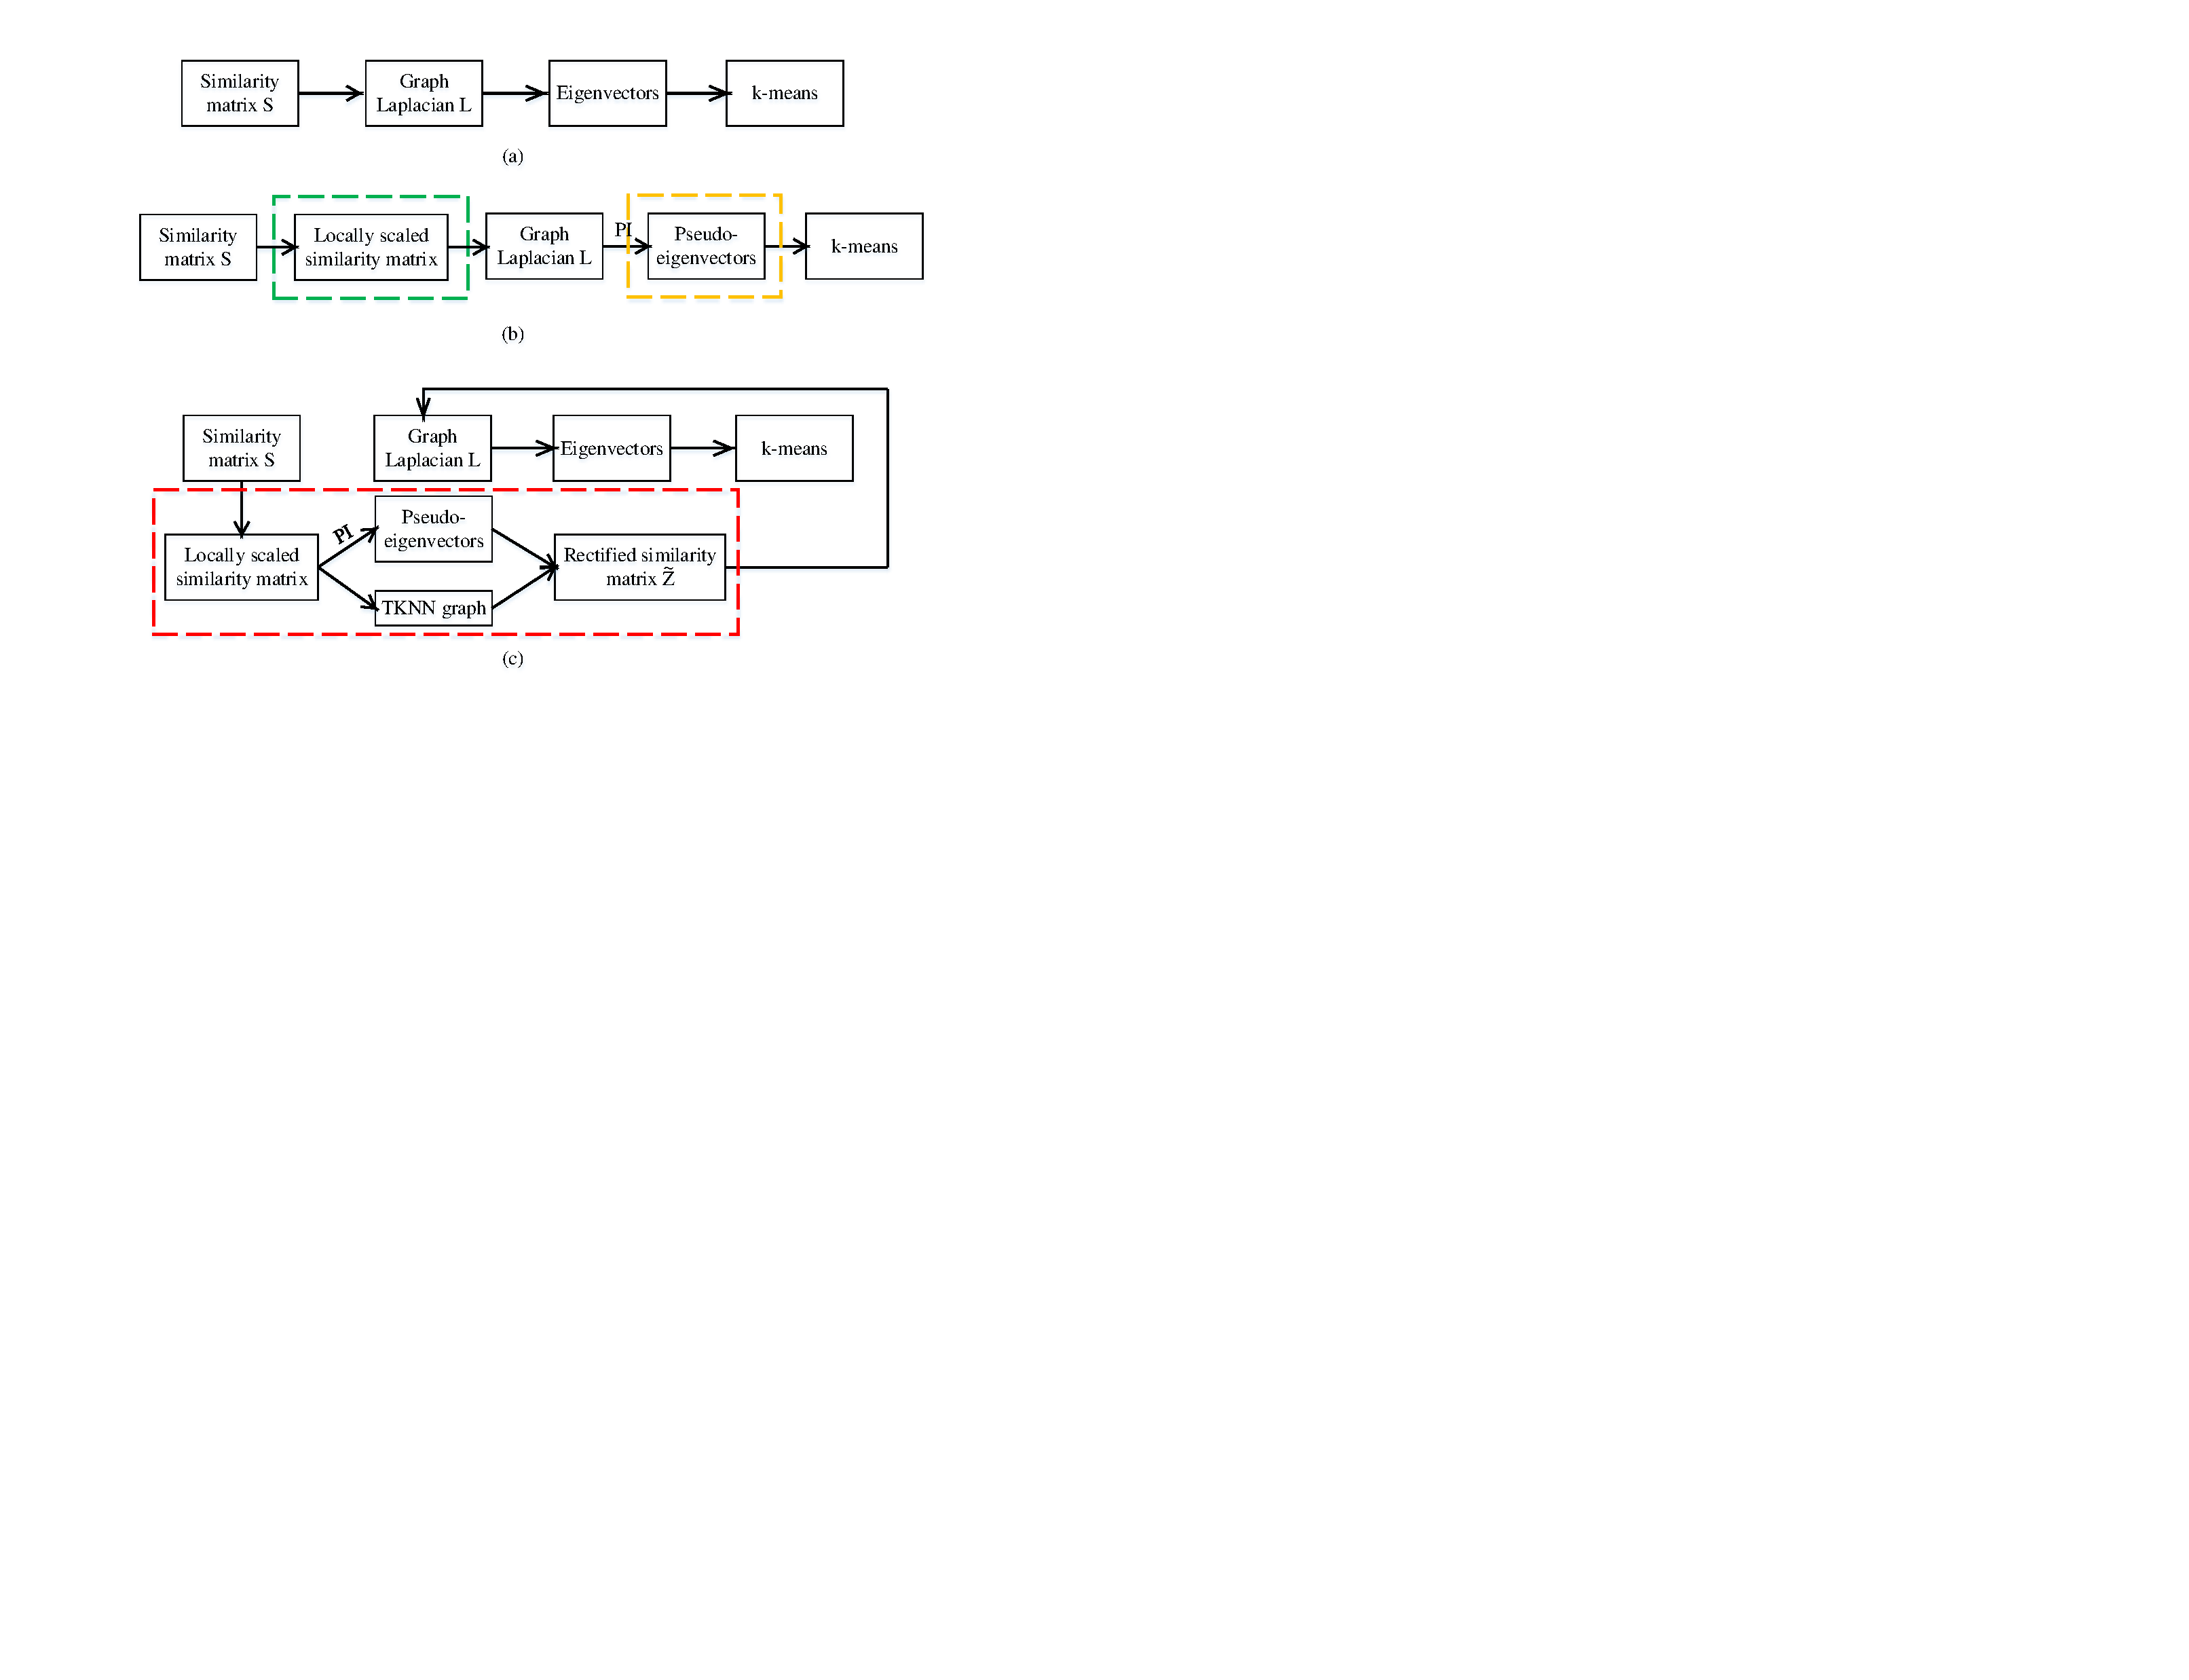
\includegraphics[width = 1.09\linewidth]{flow_graph3.pdf}
        \caption{The key steps of (a) basic spectral clustering; (b) with local scaling and PI; (c) ROSC}
        \label{figure:flow_graph}
\end{figure}
}


Our main contributions are:

\noindent$\bullet$
We proposed a heterogeneous graph convolution algorithm that is capable of capturing edge information.

\noindent$\bullet$
\dan{don't know}

\noindent$\bullet$
We conduct extensive experiments %using synthetic and real datasets 
to evaluate the performance of HINGCN
against $9$ other classification methods. 
Our results show that HINGCN performs very well against the competitors. 
In particular, it is very robust in that it consistently performs well over all the datasets tested. 
Also, it outperforms others by wide margins for datasets that are highly multi-scale. 

The rest of the paper is organized as follows.
%In Section~\ref{sec:preliminary} we give more details of spectral clustering and briefly 
%describe the power iteration method.
Section~\ref{sec:related} mentions related works on heterogeneous graph neural networks, graph embedding and described several semi-supervised classification algorithms.
Section~\ref{sec:algorithm} presents the HINGCN algorithm.
Section~\ref{sec:exp} describes the experiments and presents experimental results.
Finally, Section~\ref{sec:conclusion} concludes the paper.



%\noindent{\small$\bullet$}
%We propose a transitive $K$ nearest neighbor (TKNN) graph.
%In the graph,
%objects in the same cluster but far away in the feature space can be connected
%while objects in different clusters but close to each other can be disconnected.
%
%\noindent{\small$\bullet$}
%We put forward a robust spectral clustering method ROSC on multi-scale data.
%Based on power iteration, ROSC fuses more cluster-separation information in more eigenvectors
%and reduces the redundancy and noise contained.
%%and it integrates the noise reduction with matrix rectification.
%It further applies the TKNN graph to rectify the raw similarity matrix 
%and derives a more effective one,
%leading to a more robust spectral clustering.
%
%\noindent{\small$\bullet$}
%We conduct extensive experiments to
%prove the robustness of ROSC.
%We compare ROSC with state-of-the-art methods on both synthetic and real datasets
%with respect to three clustering measures.
%All the experimental results show that ROSC is indeed a robust spectral clustering method.

\comment{
Recently, in machine learning and computer vision areas, 
%data can be viewed as points drawn from multiple low-dimensional subspaces, with each subspace corresponding to one category or class.
subspace segmentation has been well studied,
which aims to segment (cluster) high-dimensional objects into the low-dimensional subspaces where they are drawn from.
A number of methods have been proposed, such as LRR~\cite{liu2010robust}, LSR~\cite{lu2012robust}, etc.
In these methods, given a set of data vectors $\mathcal{X} = [\bm{x}_1, \bm{x}_2,...,\bm{x}_n]$ (each column is an object) in $\mathbb{R}^d$, 
each object is represented by 
a linear combination of the basis in a dictionary $A = [\bm{a}_1,\bm{a}_2,...\bm{a}_m]$:
\begin{equation}
\nonumber
X = AZ,
\end{equation}
where $Z$ is a coefficient matrix.
Considering the case that data vectors are corrupted by noise, 
a more robust model is thus modified as 
\begin{equation}
\nonumber
X = AZ + E,
\end{equation}
where $E$ is utilized to capture noise.
Subject to the constraint, different optimization objectives on $Z$ (and $E$) are adopted by different methods,
and they desire to derive a low-dimensional mapping $Z$ which can reflect the true subspace structure in the original data.

In this paper, we aim to improve spectral clustering from both effectiveness and efficiency.
Similar to FUSE, we first use power iteration to derive a set of pseudo-eigenvectors 
which inherit all the cluster-separation information in all the eigenvectors.
Then we resort to the subspace segmentation model to purify the pseudo-eigenvectors.

To be continued.
}











\section{Related Work}
\label{sec:related}
\subsection{Semi-supervised Learning on Graphs}
\dan{TODO}
The main focus in this paper is semi-supervised classification on graphs. Given a graph with limited labels on a set of nodes, the goal of learning is to predict the label of the remaining vertices.

\dan{traditional semi-supervised classification algorithms}

Graph embedding is a class of algorithms that aims to learn low dimensional representations of vertices while preserving graph structures. In semi-supervised classification, the learnt embeddings serve as vertex features and are fed to downstream classification engines such as logistics, SVM, and MLP classifiers \dan{cite?}. There are various embedding methods designed for homogeneous graphs, which generally falls into three categories: deep neural network methods\cite{WangC016}, random walk based methods\cite{GroverL16,PerozziAS14}, matrix factorization methods and label propagation methods.

Heterogeneous graph embedding methods differ from homogeneous ones, in the sense that meta-path based structure information is considered.

\subsection{Graph Convolution Networks}
Recently, graph convolution neural networks (GCNNs) have became popular approaches in graph embedding tasks. GCNNs extend convolution neural networks (CNNs) to the graph domain and generally fall into two categories: spectral GNNs and spatial GNNs.
Spectral GNNs generally convolve on the spectrum of the graph Fourier transform. \citet{BrunaZSL13} generalizes CNNs to graphs by finding Fourier basis of graph Laplacian. 
\citet{DefferrardBV16} employs a K-order approximation to provide a localized filtering in the transformed Fourier domain.
Spatial GNNs

Attention GNNs

GCN model neatly combines graph structures and vertex features during convolution, where features of labeled vertices are propagated to unlabeled vertices through multiple layers.




%\subsection{Graph-Based semi-supervised learning}
%\dan{TODO}


















\section{Preliminary}
\label{sec:pre}

\begin{definition}
\textbf{ Heterogeneous graphs}. 
\dan{TODO}
\hfill$\Box$
\end{definition}

\begin{example}
\dan{TODO}
\end{example}

\begin{definition}
\textbf{Metapath}. 
\dan{TODO}
\end{definition}

\begin{example}
In Fig.~\ref{figure:example1},
\dan{TODO}
\end{example}












\section{Algorithm}
\label{sec:algorithm}

In this section we describe our HINGCN algorithm. Figure~\ref{figure:flow_graph}(c) shows a flow diagram of HINGCN. 
\dan{TODO:signposting}

\subsection{Edge features as supplementary information}
\label{sec:edge}
According to research findings of Xu et al. \cite{XuHLJ19}, discriminative power of a graph neural network determines its representation capability.
We claim that information is loss if we only consider adjacency of target type vertices.
Let's consider again the example shown in Fig.~\ref{figure:example}. In long tailed meta-path $APCPA$, a shrinking $A$-$A$ adjacency loses information from intermediate $PCP$ nodes. And a graph neural network using only adjacency information cannot distinguish between two instances $p_1 = (a_1 p_1 c_1 p_2 a_4)$ and $p_2 = (a_1 p_2 c_2 p_3 a_4)$. Instead, both instances are represented as edge $\langle a_1 a_4\rangle$.
Therefore we propose to improve expressivity of our network by adding additional edge feature to homogeneous $A$-$A$ edges. These edge features are designed to effectly distinguish different intermediate nodes between meta-path instances.
We propose edge features that is composed of three different components, namely path count, intermediate node embeddings and PathSim\citep{SunHYYW11}.

\noindent{\small$\bullet$}\textbf{Path Count}. Different object pairs have different numbers of path instance between them and these numbers may reflect object similarity under a given meta-path. We propose to record count of path between objects $x_u$ and $x_v$ under meta-path $\Phi$ by: 
\begin{equation*}
c(x_u,x_v) = \vert\{ p_{x_u \rightsquigarrow x_v}:p_{x_u \rightsquigarrow x_v} \vdash \Phi \}\vert
\end{equation*}

\noindent{\small$\bullet$}\textbf{Intermediate object embedding}. 
To discriminate between different intermediate objects, we propose to use a sum of pre-trained node embedding as a component of edge feature. This node embedding can be trained from heterogeneous embedding algorithms such as \cite{GroverL16,DongCS17}.
Given a meta-path instance $p = (x_1x_2\ldots x_{l+1})$, we calculate
\begin{equation*}
o(x_1,x_{l+1}) = \dfrac{1}{(l+1) \cdot c(x_1,x_{l+1})} \sum\limits_{i=1}^{l+1} e_i
\end{equation*}
where $e_i$ is embedding of object $x_i$. Division of number of vertices $l+1$ and path count $c(x_u,x_v)$ is proposed to normalize intermediate object embedding to the scale of input object embeddings. Since path count is extracted and recorded as $c(x_u,x_v)$, this does no result in extra loss of information.

\noindent{\small$\bullet$}\textbf{PathSim}. 
PathSim is proposed in \citep{SunHYYW11} to measure similarity between two objects of a same type on a heterogeneous graph. Given a symmetric meta-path $\Phi$, PathSim between $x_u$ and $x_v$ is:
\begin{equation*}
s(x_u,x_v) = \frac{2\times\vert\{ p_{x_u \rightsquigarrow x_v}:p_{x_u \rightsquigarrow x_v} \vdash \Phi \}\vert}{\vert\{ p_{x_u \rightsquigarrow x_u}:p_{x_u \rightsquigarrow x_u} \vdash \Phi \}\vert +\vert\{ p_{x_v \rightsquigarrow x_v}:p_{x_v \rightsquigarrow x_v} \vdash \Phi \}\vert }
\end{equation*}

The edge feature between objects $x_u$ and $x_v$ under meta-path $\Phi$ is thereby concatenated as:
\begin{equation}
\label{eq:edge}
r^{(0)}_\Phi(x_u,x_v) = c(x_u,x_v)\oplus o(x_u,x_v)\oplus s(x_u,x_v)
\end{equation}

\subsection{Aggregating node embedding}
We propose a modified version of scaled dot product attention mechanism to aggregate node embedding from its neighbor. Given a meta-path $\Phi$, we update vertex embedding as follow. First we apply 2 layer MLPs on node embedding and its neighbor respectively for scaling purpose. The query vector of node $i$ is
\begin{equation}
q_i= W_{a1}^{(t)}(\text{tanh}(W_{a2}^{(t)}h^{(t)}_i ))
\end{equation}
And key vector $k_{i,j}$ is calculated as:
\begin{equation}
k_{i,j} = W_{a3}^{(t)}(\text{tanh}(W_{a4}^{(t)}(h^{(t)}_j \oplus r^{(t)}_{i,j}) ))
\end{equation}
And the value vector of neighbor $j$ is calculated as: 
\begin{equation}
\label{eq:value}
v^{(t)}_{i,j} = W^{(t)}( h^{(t)}_j \oplus r^{(t)}_{i,j} )
\end{equation} 
where edge feature $r^{(t)}_{i,j}$ is concatenated to vertex feature of the neighbors, in order to provide additional information. It is worth noticing that due to unique feature of each edge, both key and value vectors are no longer universal for different query nodes. We believe this uniqueness improves expressivity of self-attention mechanism for HIN embedding tasks.

\noindent Afterwards, the importance of a neighbor $j$ to object $i$ is calculated as:
\begin{equation}
\label{eq:dot}
\tilde{a}^{(t)}_{i,j} = q_i^T \cdot k_{i,j}
\end{equation}
Then we normalize this importance coefficient by softmax function and calculate attention coefficient as:
\begin{equation}
\label{eq:softmax}
a^{(t)}_{i,j} = \text{softmax}(\tilde{a}^{(t)}_{i,j}) = \dfrac{\text{exp}(\tilde{a}^{(t)}_{i,j})}{\sum_{k\in N^\Phi_i}\text{exp}(\tilde{a}^{(t)}_{i,k})}
\end{equation}
Finally the output of the node aggregation layer is a weighted sum of value vectors. 
\begin{equation}
\label{eq:upd_node}
h^{(t+1)}_i = \text{ReLU}(W_{h2}\cdot h^{(t)}_i + W_{h1}\cdot \sum_{j\in N^\Phi_i} a^{(t)}_{i,j} \cdot v^{(t)}_{i,j} ) 
\end{equation} 
Although a vertex $i$ is always in its own meta-path neighbor, we still explicitly add term $h^{(t)}_i$ in equation \ref{eq:upd_node} following GraphSAGE\cite{HamiltonYL17}.

\subsection{Aggregating edge embedding}
\dan{TODO} In multi-layer propagation, we propose to update embeddings of edge as well.
\begin{equation}
\label{eq:upd_edge}
r^{(t+1)}_{i,j} = \text{ReLU}(W_{r1}\cdot (h^{(t)}_i \oplus h^{(t)}_j \oplus r^{(t)}_{i,j}) + W_{r2}\cdot r^{(t)}_{i,j}) 
\end{equation} 

\subsection{Dealing with over-smoothing via adaptive depth}
\dan{TODO:relate this example to the example figure used in preliminary section}
Plain GCNs often degrades rapidly as number of layers increases \cite{LiHW18,abs-1904-03751}. Stacking four or more layers into GCNs cause over-smoothing problem and features of vertices tends to converge to the same value. In heterogeneous graphs, this problem is even more severe. Let's consider again meta-path $APCPA$ in Fig.~\ref{figure:example}. A two layer $a_1 a_2 a_3$ propagation on the shrinking $A-A$ homo-graph actually passes across \textbf{8} edges on the underlying heterogeneous graph, which is a terrible number of layers for plain graph convolution networks.
To alleviate the over-smoothing problem, in equation \ref{eq:upd_node} and \ref{eq:upd_edge}, we have already included residual connections \cite{HeZRS16} in updating rule. And we propose to further improve the problem by creating jumping connections \cite{XuLTSKJ18}.
\begin{equation}
\label{eq:jump}
h^{(final)}_i = h^{(0)}_i \oplus h^{(1)}_i \cdots \oplus h^{(t)}_i
\end{equation} 

\subsection{Aggregation across different meta-path semantics}
\dan{need some intuition/justification shit}
Given a node $i$, and its set of embeddings under different semantics, a metapath aggregator is a function $\gamma$ in the form of $y_i = \gamma_\Theta(\{x_{i,1},x_{i,2},..x_{i,P}\})$, where $x_{i,p}$ is the embedding of node $i$ under metapath $p$, and $y_i$ is the aggregated embedding of node $i$ in the HIN. $\Theta$ is the learnable paremeters of the aggregator.
Here we propose several metapath aggregators. 

$\bullet$ \textbf{Attention}
\dan{cite} The first option we consider is scaled dot-product attention introduced in Transformer. 
\begin{equation}
\label{eq:mp_mlp}
\tilde{h}^{\Phi_p}_i = W_{m1} \cdot \text{tanh}(W_{m2} \cdot h^{\Phi_p}_i)
\end{equation}

\begin{equation}
\label{eq:mp_attn}
\tilde{w}_i^{\Phi_p} = W_w \cdot \sigma(\tilde{h}^{\Phi_p}_i)
\end{equation}

\begin{equation}
\label{eq:mp_soft}
w_i^{\Phi_p} = \text{softmax}(\tilde{w}_i^{\Phi_p}) = \dfrac{\text{exp}(\tilde{w}_i^{\Phi_p})}{\sum_q \text{exp}(\tilde{w}_i^{\Phi_q})}
\end{equation}

After the fully-connected self-attention, we propose to reduce across different meta-path semantics by \textbf{Sum} operation.
\begin{equation}
\label{eq:mp_asum}
z_i = \text{ReLU}(\sum_p w_i^{\Phi_p} \cdot h^{\Phi_p}_i)
\end{equation}

$\bullet$ \textbf{Gated linear unit}
Inspired by forget gate mechanisms in recurrent networks (RNN) \dan{TODO:cite}, we compute a soft gate between 0 (low importance) and 1 (high importance) to represent different importance to each embedding entry.
We make the element-wise gated sum layer as follows:
\begin{multicols}{2}
\begin{equation}
o^{\Phi_p}_i=\sigma(W_o \cdot h^{\Phi_p}_i)
\end{equation}\break
\begin{equation}
\tilde{h}^{\Phi_p}_i=\text{tanh}(W_z \cdot h^{\Phi_p}_i)
\end{equation}
\end{multicols}
Finally, we have
\begin{equation}
\label{eq:mp_sum}
{z}_i= \sum_p o^{\Phi_p}_i\odot \tilde{h}^{\Phi_p}_i
\end{equation}

The gated unit $o_{\Phi_p}$ with sigmoid output (ranged (0,1)) is used to control which elements are to be aggregated in the output. 
 
$\bullet$ \textbf{Other aggregators}
In preliminary experiments, \textbf{Concat}, \textbf{Max-Pooling} and \textbf{Mean} aggregators did not generate a better result, and we omit results of these aggregators in experiment section.

\subsection{HINGCN: Semi-supervised classification on Heterogeneous Information Network via Graph Convolution Networks}
After meta-path aggregation layer, the embeddings are fed to a 2-layer MLP for final output. In semi-supervised classification tasks, we minimize the Cross-Entropy loss and the model generates final prediction based on the largest output value.
\begin{equation}
\label{eq:loss}
\mathcal{L}(W)=   - \sum_{l\in \mathcal{Y}_L}Y^l ln(z^l)   + \lambda \parallel W \parallel_2
\end{equation}
$ \mathcal{Y}_L$ is the set of labeled nodes in training set. $W$ represents the weight matrices used in the layers of our HINGCN. We use $L_2$ normalization for parameters involved.

To this end, HINGCN is summarized in Algorithm~\ref{alg}.
HINGCN first computes initial edge feature $r^{(0)}_{\Phi_p}$ for each edge under each meta-path. Then it applies an alternative update of node embedding and edge embedding.
After that each node fuses a meta-path specific embedding by jumping connections. These embeddings are further aggregated using either meta-path level attention or gated linear units. Finally, embeddings are fed to a two layer MLP and a softmax layer for classification output.

\dan{TODO}
\begin{algorithm}
\begin{small}
\caption{Overall process of HINGCN}
\label{alg}
\begin{algorithmic}[1]
\Require Labeled type $T$;
meta-path set ${\Phi_0,\Phi_1,\ldots ,\Phi_P}$;
an initial node representation $\{ f_i,\forall x_i \in X_T \}$;
number of aggregation layers $L$;
\Ensure $\mathcal{C} = \{C_1, ..., C_k\}$
\State Compose edge features $r^{(0)}$ according to Equation (\ref{eq:edge})
\State $h^{(0)}_i \leftarrow f_i$, $\forall x_i \in $
\For $j \leftarrow 1$ do
\State Calculate $W = D^{-1}S$, where $D_{ii} = \sum_jS_{ij}$
\EndFor
%\For $j \leftarrow 1$ do
%\State$t = 0$
%\Repeat
%\State $v_j^{t+1} \leftarrow \frac{Wv_j^t}{||Wv_j^t||_1}$
%\State $ \delta^{t+1} \leftarrow |v_j^{t+1} - v_j^t|$
%\State $t$++
%\Until $||\delta_j^t+1 - \delta_j^t||_{max} \leq \epsilon$ or $t\geq T$
%\EndFor
\State Computes initial edge feature $r^(0)_{\Phi_p}$
\For $j \leftarrow 1$ do

\EndFor
\State Normalize each column vector $\bm{x}$ of $X$ such that $\bm{x}^T\bm{x} = 1$
\State Calculate the coefficient matrix $Z^*$ by Eq.~\ref{eq:solution}
\State Construct $\tilde{Z} = (|Z^*| + |(Z^*)^T|)/2$
\State Run standard spectral clustering methods, e.g., NCuts, with $\tilde{Z}$ as the
similarity matrix to obtain clusters $\mathcal{C} = \{C_r\}_{r=1}^k$
%\State Decode $\{C_r\}_{r=1}^k$ from $\{{\bm z_r}\}_{r=1}^k$
\State \Return $\mathcal{C} = \{C_1, ..., C_k\}$
\end{algorithmic}
\end{small}
\end{algorithm}










\section{Experiment}
\label{sec:exp}
We conducted extensive experiments
to evaluate the performance of HINGCN.
This section summarizes our results. 
We compare the various methods using three popular measures, 
namely, \emph{accuracy}, \emph{micro-F1}, and \emph{macro-F1}.
These measures evaluate clustering quality and their values range from 0 to 1, 
with a larger value indicating a better
clustering quality. 
%We first describe the performance measures (Section~\ref{sec:measures}) and
%existing methods against which ROSC is compared (Section~\ref{sec:algo-comp}).
%We then show the performance results on both real and synthetic datasets (Section~\ref{sec:results}).
%We illustrate the grouping effect of matrix $\tilde{Z}$ (Section~\ref{}).
%Finally, we conduct a parameter sensitivity study of ROSC (Section~\ref{}).

\subsection{Datasets}
A summary of statistics of the datasets rae shown in table \ref{table:dataset}.

\noindent{\small$\bullet$}
\textbf{DBLP}: We extract a subset of DBLP with contains 4057 authors ($A$), 14328 papers ($P$) and 20 conferences ($C$). 8789 terms of papers are aggregated to each author as feature, after tf-idf transformation. Here we select meta-paths $\{APA,APAPA,APCPA\}$ for experiments.

\noindent{\small$\bullet$}
\textbf{Yelp}: A standard spectral clustering method with symmetric normalization.

\noindent{\small$\bullet$}
\textbf{Freebase}: A standard spectral clustering method with symmetric normalization.

\comment{
\subsection{Measures}
\label{sec:measures}
We use three popular measures, namely, \emph{purity}, \emph{adjusted mutual information (AMI)}, and \emph{rand index (RI)}, to evaluate clustering quality~\cite{vinh2010information,lin2010power}.

Consider a clustering $\mathcal{C} = \{C_1, \ldots, C_k\}$ produced by a clustering algorithm
and a gold standard (true) clustering
$\mathcal{C}_t = \{ \hat{C}_1, \ldots, \hat{C}_k\}$.
For each cluster $C_i \in \mathcal{C}$, we find the cluster $\hat{C}_j \in \mathcal{C}_t$ that overlaps
with $C_i$ the most. 
The purity of cluster $C_i$ is the fraction of objects in $C_i$ that fall in the overlap, i.e., 
($\max_j |C_i \cap \hat{C}_j|) / |C_i|$. 
The purity of a clustering $\mathcal{C}$ is the average of its clusters' purities, weighted by the cluster sizes:
\begin{equation}
purity(\mathcal{C}_t,\mathcal{C}) = \frac{1}{n}\sum_{i}\max_{j}|C_i \cap \hat C_j|.
\end{equation}
The adjusted mutual information ({\it AMI}) is mutual information with the agreement due to chance between clusterings corrected, and
is given by,
\begin{equation}
\mathit{AMI}(\mathcal{C}_t,\mathcal{C}) = \frac{MI(\mathcal{C}_t,\mathcal{C}) - E\{MI(\mathcal{C}_t,\mathcal{C})\}}{\max\{H(\mathcal{C}_t),H(\mathcal{C})\} - E\{MI(\mathcal{C}_t,\mathcal{C})\}},
\end{equation}
where $MI(\mathcal{C}_t,\mathcal{C})$ is the mutual information between $\mathcal{C}_t$ and $\mathcal{C}$,
$H(\mathcal{C}_t)$ and $H(\mathcal{C})$ are the entropies of $\mathcal{C}_t$ and $\mathcal{C}$, respectively,
and $E\{MI(\mathcal{C}_t,\mathcal{C})\}$ is the expected mutual information between the two clusterings
$\mathcal{C}_t$ and $\mathcal{C}$.

Rand index ({\it RI}) considers object pairs in measuring clustering quality. It is defined as:
\begin{equation}
RI(\mathcal{C}_t,\mathcal{C}) = (N_{00} + N_{11}) / {\tbinom n2},
\end{equation}
where $N_{00}$ is the number of object pairs that are put into the same cluster in $\mathcal{C}_t$
as well as in the same cluster in $\mathcal{C}$, and
$N_{11}$ is the number of object pairs that are put into different clusters in 
$\mathcal{C}_t$ and also in different clusters in $\mathcal{C}$.
Note that values of all three measures range from 0 to 1, with a larger value indicating a better
clustering quality. 
}

\subsection{Algorithms for comparison}
\label{sec:algo-comp}
We evaluate HINGCN and 9 other methods.
These methods are grouped into the following four categories.
%
%\noindent$\bullet$
%\textbf{(Random walk based network embedding methods)}: 
%{\bf NCuts} and {\bf NJW} are two standard methods we evaluate against ROSC.
%%which follow the execution pipelines shown
%%in Figure~\ref{figure:flow_graph}(a). 
%
%\noindent$\bullet$
%\textbf{(Power iteration (PI) based methods)}: 
%This group includes {\bf PIC}, {\bf PIC-$k$}, {\bf DPIC}, and {\bf DPIE}. 
%They were described in Section~\ref{sec:related}.
%%PIC is a PI based method which generates only one pseudo-eigenvector.
%%In comparison, PIC-\emph{k} generates $\lceil log(k)\rceil$ pseudo-eigenvectors.
%%DPIC employs Schur complement deflation to generate mutually orthogonal pseudo-eigenvectors.
%%Finally, DPIE generates a set of diverse pseudo-eigenvectors.

%\noindent$\bullet$
%\textbf{(Multi-scale-data-oriented methods)}: 
%This group includes {\bf ZP} and {\bf FUSE}, which are designed to specifically handle multi-scale data.
%They were also discussed in Section~\ref{sec:related}.
%Note that ZP automatically estimates the number of clusters.
%For fairness, we modify ZP so that it returns $k$ (the number of true) clusters.
%
%
%ZP is a self-tuning spectral clustering method which considers the local scale information for objects in multi-scale data.
%It can automatically estimate the number of clusters.
%To make a fair comparison, we directly set $k$ as in other methods.
%Although FUSE is based on PI, 
%it further uses ICA to rotate the pseudo-eigenvectors to make them pair-wise statistically independent.
%The rotated pseudo-eigenvectors can lead to desiring performance on multi-scale data.
%
%\noindent$\bullet$
%\textbf{(ROSC variants)}: 
%{\bf ROSC} regularizes matrix $Z$ using the reachability matrix.
%This is achieved via the term $||Z-\mathcal{W}||_F^2$ in Equation~\ref{eq:obj_constraint}. 
%%we see that the rectification of matrix $Z$ involves three components.
%%In particular, the first term ($||X-XZ||_F^2$) models noise reduction, while the third ($||Z-\mathcal{W}||_F^2$)
%%regularizes $Z$ with the reachability matrix. 
%To study the regularization effect, we modify ROSC with this term
%removed. 
%Specifically, {\bf ROSC-R} (reads ``ROSC minus reachability'') is ROSC without the reachability component.
%%{\bf ROSC-NR} (reads ``ROSC minus noise reduction'') is ROSC without noise reduction.


\noindent{\small$\bullet$}
\textbf{NJW}: A standard spectral clustering method with symmetric normalization.

\noindent{\small$\bullet$}
\textbf{NCuts}: A standard spectral clustering method with divisive normalization.

\noindent{\small$\bullet$}
\textbf{ZP}: A self-tuning spectral clustering method for multi-scale clusters.
It uses eigenvector rotation to estimate the number of clusters.
To make a fair comparison, we directly set $k$ as in other methods.

\noindent{\small$\bullet$}
\textbf{PIC}: A power iteration based method which generates only one pseudo-eigenvector.

\noindent{\small$\bullet$}
\textbf{PIC-$k$}:
A power iteration based method which generates $\lceil log(k)\rceil$ pseudo-eigenvectors.

\noindent{\small$\bullet$}
\textbf{DPIC}: 
A power iteration based method which employs Schur complement deflation to generate mutually orthogonal pseudo-eigenvectors.

\noindent{\small$\bullet$}
\textbf{DPIE}: A power iteration based method which generates a set of diverse pseudo-eigenvectors.
%As suggested by~\cite{huang2014diverse}, 
%we set the maximum number of pseudo-eigenvectors to be $\lceil log(k) \rceil * 6 $ 
%out of $\max(\lceil log(k) \rceil * 30, 2k)$ random initial vectors.

\noindent{\small$\bullet$}
\textbf{FUSE}:
A full spectral clustering method based on power iteration and ICA. 


\textbf{[Experiment settings]} The parameters of all the methods are set according to their original papers.
%For text data, cosine similarity is used to calculate the similarity matrix $S$.
%For attributed data, 
For all the datasets,
we use Euclidean distance of objects' attributes to derive $S$,
which are locally scaled based on ZP's local scaling procedure.
For ROSC, we set $\alpha_1 = 1.0$, $\alpha_2 = 0.01$, and we set $K=4$ in constructing TKNN graphs. 
All methods adopt \emph{k}-means as the last step to return clustering results.
For this step, 
we run \emph{k}-means $100$ times with random starting centroids
and the most frequent cluster assignment is used~\cite{lin2010power}.
For ROSC, we generate $k$ pseudo-eigenvectors with random starting vectors as is done in~\cite{thang2013deflation}.
For each method and dataset,
we run the experiment 50 times and report average results.

\subsection{Performance results}
\label{sec:results}
%\subsection{Clustering on synthetic datasets}

We first use two synthetic datasets to visually illustrate the performance of the various methods. 
After that, we use 7 real datasets to perform an in-depth analysis of the algorithms.

\noindent{\bf[Synthetic datasets]}
The synthetic datasets are designed to represent very difficult cases of clustering, with a highlight
on multi-scale data. 
Figure~\ref{figure:syn2}(a) shows the synthetic dataset \textsc{Syn1}, which consists of three clusters of
different sizes and densities. 
Specifically, there is a medium-sized sparse rectangular cluster (blue) sandwiched by a small dense circular
cluster (magenta) and a large dense rectangular one (yellow). These clusters are physically very close to each other. 
In particular, the distance between two objects of different clusters could be smaller than the distance of
two objects that belong to the same cluster.  

We apply all 10 methods on \textsc{Syn1}. 
Due to space limitations, for each category of methods, we only show the best performing one. 
They are, namely, NJW, PIC-$k$, FUSE, and ROSC. 
Their clustering results are shown in Figures~\ref{figure:syn2}(b)-(e), respectively. 
From the figures, we see that both NJW and PIC-$k$ can identify the small circular magenta cluster. 
However, the blue and the yellow rectangular clusters are chopped into halves, and these halves are
incorrectly merged. FUSE fails for this dataset as well. 
In particular, about 1/3 of the yellow cluster is merged with the blue cluster, while about half of the
blue cluster is merged with the magenta cluster. 
Among the four methods, ROSC is the only one that can recover the yellow cluster. 
This indicates the effectiveness of the TKNN graph in correlating objects that are at the far ends of 
the big elongated cluster. 
Moreover, although ROSC does not recover the complete blue cluster, a majority fraction of the
blue objects are clustered by ROSC as a single group. 
In contrast, for the other three methods, all blue objects are either merged with those of the magenta cluster
or those of the yellow cluster.

\begin{figure*}[!htbp]
    \centering
        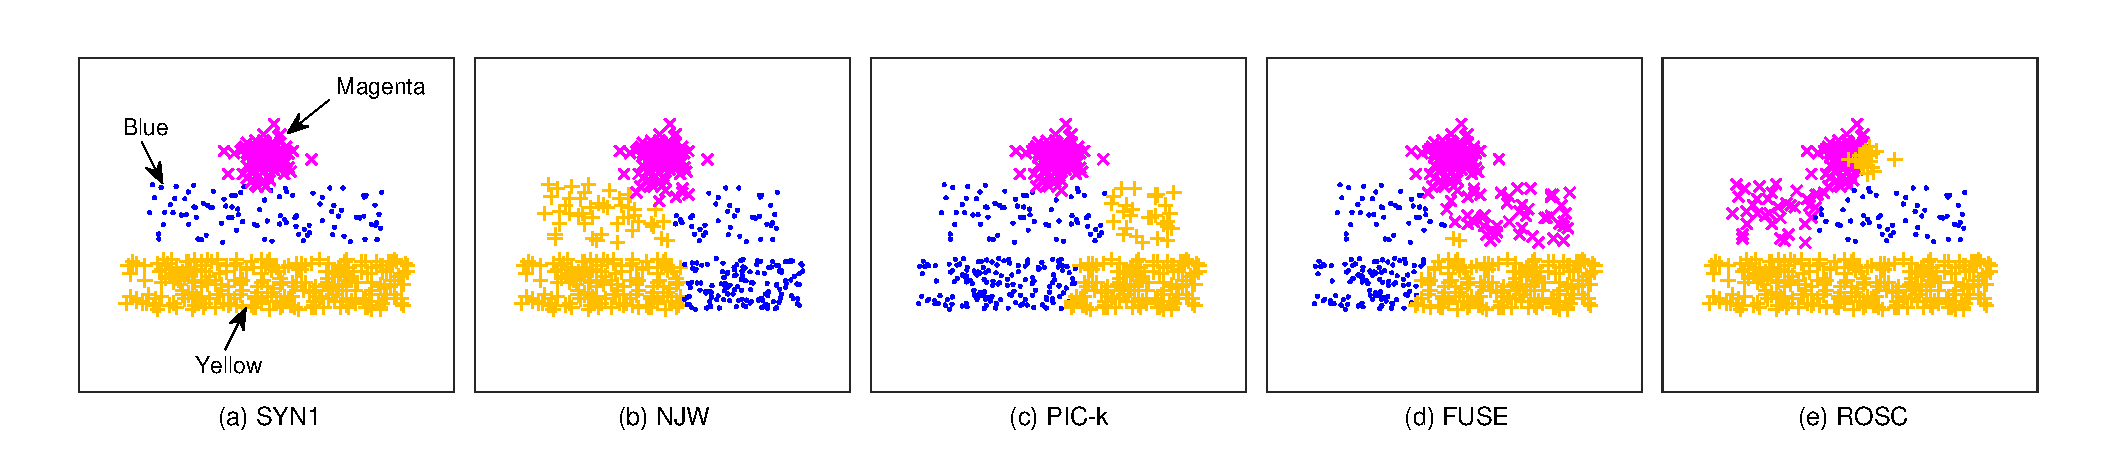
\includegraphics[width = 0.9\linewidth]{figure/syn2_res_new1.eps}
        \caption{Clustering results on \textsc{Syn1}}
        \label{figure:syn2}
%\end{figure*}

%\begin{figure*}[!htbp]
    %\centering
        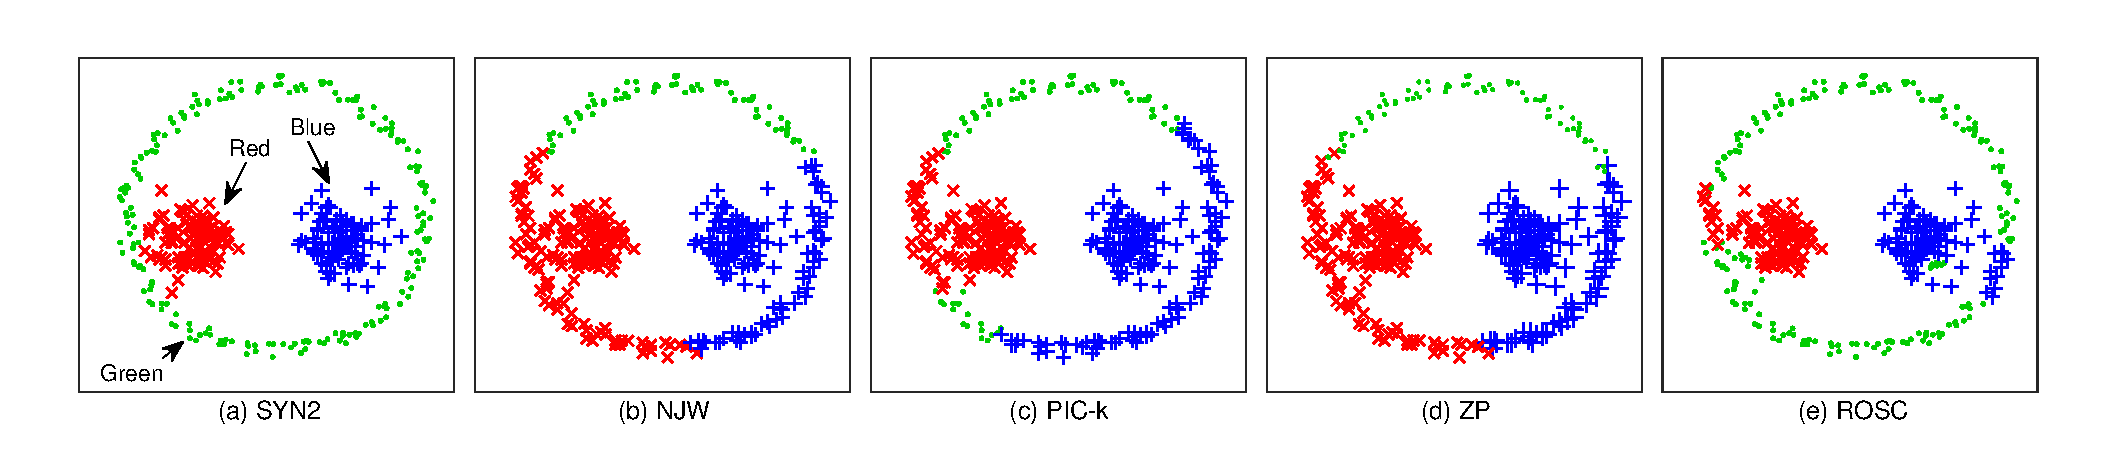
\includegraphics[width = 0.9\linewidth]{figure/syn3_res_new.eps}
        \caption{Clustering results on \textsc{Syn2}}
        \label{figure:syn3}
%\end{figure*}

\comment{
%\begin{figure*}[!htbp]
   % \centering
        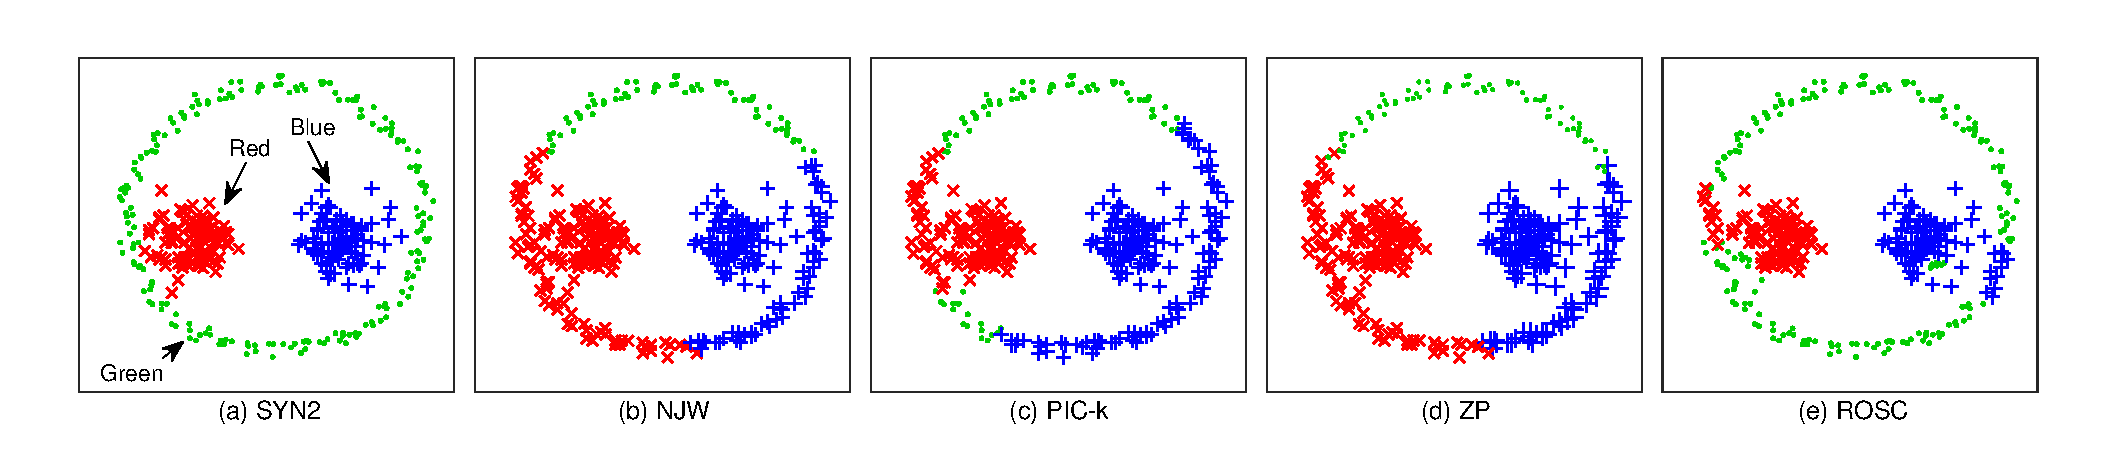
\includegraphics[width = \linewidth]{figure/syn3_res_new.eps}
        \caption{Clustering results on \textsc{Syn3} (shown are the most frequent results)}
        \label{figure:syn3}
%\end{figure*}

\begin{figure*}[!htbp]
    \centering
        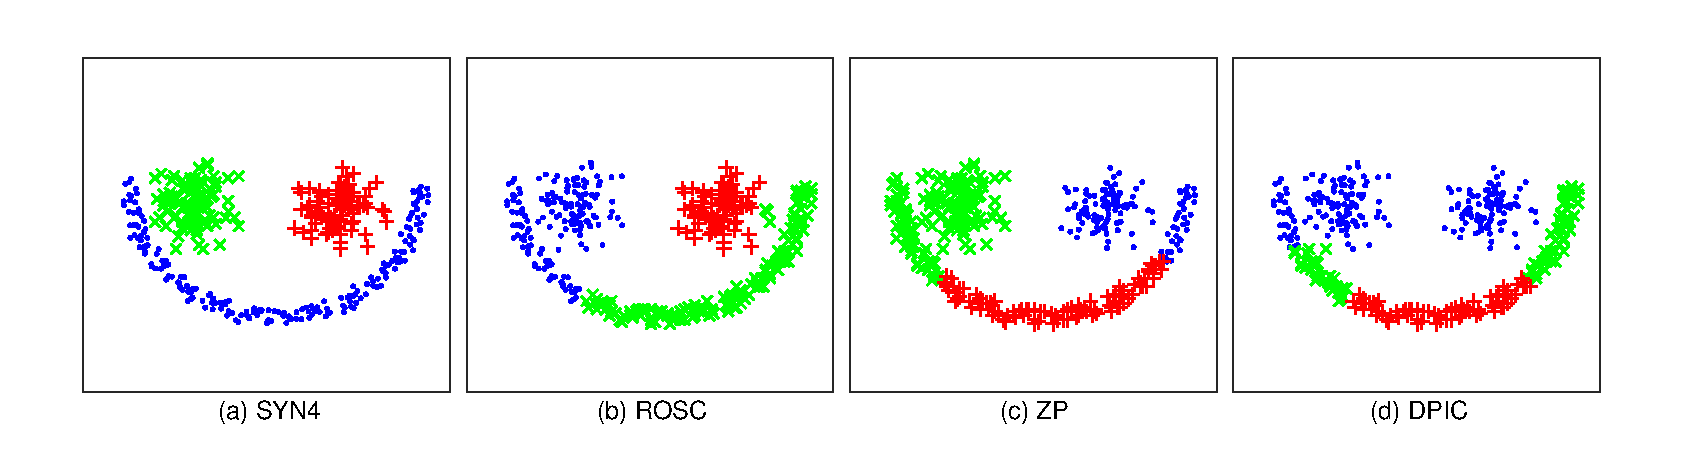
\includegraphics[width = \linewidth]{figure/syn4_res.eps}
        \caption{Clustering results on synthetic dataset 4 (shown are the most frequent results)}
        \label{figure:syn4}
 }
\end{figure*}


\begin{table*}[!htbp]
\centering
\resizebox{0.9\linewidth}{!}
{
\begin{tabular}{|c||c|c||c|c|c|c||c|c||c|c|} \hline
Measure &NJW & NCuts & PIC & PIC-$k$ & DPIC & DPIE & ZP & FUSE & ROSC-R & ROSC \\ \hline 
Purity & $0.8000$ & $0.8000$ &  $0.7262$ & $0.7772$ & $0.6663$ & $0.6348$ & $0.8000$ & $0.7688$ & $0.7594$ & $\bm{0.8538}$\\ \hline
AMI    & $0.4338$ & $0.4256$ &  $0.3941$ & $0.4686$ & $0.2502$ & $0.1381$ & $0.4232$ & $0.4873$ & $0.4331$ & $\bm{0.6255}$ \\ \hline
RI       & $0.6811$ & $0.6817$ & $0.6513$ & $0.6901$ & $0.5786$ & $0.4707$ & $0.6812$ & $0.6837$ & $0.6762$ & $\bm{0.8354}$\\ \hline
\end{tabular}
}
\caption{Purity, AMI, and RI scores of methods for dataset \textsc{Syn1}}
\label{table:syn1}
\resizebox{0.9\linewidth}{!}
{
\begin{tabular}{|c||c|c||c|c|c|c||c|c||c|c|} \hline
Measure &NJW & NCuts & PIC & PIC-$k$ & DPIC & DPIE & ZP &  FUSE & ROSC-R & ROSC\\ \hline 
Purity & $0.6775$ & $0.6775$ & $0.6541$ & $0.6849$ & $0.5196$ & $0.5171$ & $0.6875$ & $0.6773$ & $0.7002$ & $\bm{0.8359}$\\ \hline
AMI    & $0.4681$ & $0.4679$ & $0.4157$ & $0.4740$ & $0.2136$ & $0.1320$ &$0.4746$ &  $0.4554$ & $0.4602$ & $\bm{0.6178}$\\ \hline
RI       & $0.6725$ & $0.6724$ & $0.6477$ & $0.6789$ & $0.4866$ & $0.4392$ & $0.6780$ & $0.6683$ & $0.6909$ & $\bm{0.8056}$\\ \hline
\end{tabular}
}
\caption{Purity, AMI, and RI scores of methods for dataset  \textsc{Syn2}}
\label{table:syn2}
\end{table*}


Figure~\ref{figure:syn3}(a) shows another synthetic dataset, \textsc{Syn2}, which consists of
a sparse ring cluster (green) and two dense circular clusters (red and blue). 
The best performing methods of the 4 categories are NJW, PIC-$k$, ZP, and ROSC.
Their clustering results are shown in Figures~\ref{figure:syn3}(b)-(e), respectively.
From the figures, we see that the dataset is a very difficult case for existing methods. 
For example, with NJW and ZP, the green ring cluster is partitioned into three segments, two of which 
are merged incorrectly with the circular clusters. A similar situation is also seen for PIC-$k$. 
In contrast, ROSC is the only method that can recover almost the entire green cluster. 
It is also able to correctly identify the two circular clusters except for a small number of 
objects on the green ring. 

Tables~\ref{table:syn1} and \ref{table:syn2} show the purity, AMI and RI scores of all 10 methods
for the datasets \textsc{Syn1} and \textsc{Syn2}, respectively. 
From the tables, we see that the scores of ROSC are all much larger than those of the other methods.
It thus significantly outperforms the others for these two difficult cases. 
The two tables also show the scores of ROSC-R, which is ROSC without using the TKNN graph or
the reachability matrix for regularization. Considering the wide gaps between the scores of ROSC and
ROSC-R, we see a strong positive effect of the reachability regularization. 
The use of TKNN graph and reachability has a significant effect in the two synthetic datasets because
both datasets consist of large elongated clusters (e.g., the green ring in \textsc{syn2}).
Objects in these clusters are at far distances from each other and their correlations are effectively captured by
the reachability matrix that ROSC employs.
 
We further investigate how the various methods deal with multi-scale data by varying the sizes and densities
of some clusters in the synthetic datasets. 
Here, we show some representative results. 
Specifically, we consider the middle sparse blue cluster in \textsc{Syn1} (Figure~\ref{figure:syn2}(a))
and make two changes: 
(1) increase its density while keeping its size unchanged, and
(2) increase its size while maintaining its density unchanged.
We use $\Delta d$ to denote the density change
(e.g., $\Delta d$ = 100\% means that the density of the cluster is doubled).
We change the size of the cluster by changing its length
(enlarging the cluster sideway), while the height is kept unchanged.
We use $\Delta s$ to denote the size change
(e.g., $\Delta s$ = 50\% means that the cluster is 1.5 times wider than the one shown in Figure~\ref{figure:syn2}(a)).
We make similar changes to \textsc{Syn2} by modifying the density and size of the ring cluster. 
Specifically, we gradually reduce the size of the ring from a whole ring ($\bigcirc$, $\Delta s$ = 0\%)
to a lower half ring ($\smile$, $\Delta s$ = -50\%).

We show the performance scores of the 10 methods 
as we apply the changes in density and size to the clusters in \textsc{Syn1}
(Figures~\ref{figure:syn2_d} and \ref{figure:syn2_s})
 and \textsc{Syn2}
 (Figures~\ref{figure:syn3_d} and \ref{figure:syn3_s}).
From the figures, we see 
that  ROSC gives the best and the most stable performance among all the methods 
over the whole spectrum of test cases. 
The performance gaps between ROSC and other competitors are also sizable. 
This shows that ROSC is very robust in dealing with multi-scale data of various sizes and densities.
 
%We further explore the robustness of ROSC on multi-scale data
%by studying how the cluster density and size influence the performance of spectral clustering.
%Based on the synthetic datasets, we conduct two groups of experiments.
%First, vary the cluster density with the cluster size fixed.
%Second, vary the cluster size with the cluster density fixed.
%It is also emphasized that
%each time we only vary one cluster with other clusters fixed.
%For example,
%we vary the cyan cluster in \textsc{Syn1} and the circular cluster in \textsc{Syn2} with other clusters fixed.
%To flexibly control the cluster density and size,
%clusters to be varied are set as uniformly distributed.
%Experimental results are shown in
%Fig.~\ref{figure:syn2_d} -~\ref{figure:syn3_s}. 
%$\Delta d$ and $\Delta s$ denote the growth rate in density and size respectively.
%%In \textsc{Syn1}, the strip cluster is so narrow that we explore much larger $\Delta s$ than in other two datasets.
%With varied density and size,
%ROSC consistently outperforms all the comparison methods in all cases,
%%on \textsc{Syn1} and \textsc{Syn2},
%%and performs the best in most cases on \textsc{Syn3}, 
%which proves its robustness convincingly.


\comment{
Experimental results on \emph{AMI}, \emph{purity} and \emph{RI} are respectively 
summarized in Table~\ref{table:ami_synthetic},~\ref{table:purity_synthetic} and~\ref{table:ri_synthetic}.
To better present the results,
we select some methods and show their results graphically. 
%in Fig.~\ref{figure:syn1},~\ref{figure:syn2},~\ref{figure:syn3} and~\ref{figure:syn4}. 

The first dataset consists of 
three uniformly distributed clusters with 500, 80 and 120 objects respectively.
Since the largest rectangular cluster is of large length,
the two-end objects in the cluster are far away from each other,
i.e., they are less similar. 
Further, the closeness between the two small clusters and the large cluster increases more difficulty in clustering.
We observe that 
ROSC achieves $0.4384$ in AMI, $0.8515$ in purity and $0.7121$ in RI,
which outperforms all the comparison methods.
From Fig.~\ref{figure:syn1},
both ZP and FUSE perform poorly in that they separate the large cluster into small subclusters.
In comparison, ROSC correctly identifies the largest cluster.

The second dataset shown in Fig.~\ref{figure:syn2}(a)
is composed of five clusters:
two Gaussian distributed with 100 objects each,
two uniformly distributed with 150 and 200 objects respectively 
and an annular cluster with 100 objects.
The annular cluster is close to the other clusters and it is hard to be identified.
Experimental results show that ZP is the best method on this dataset. 
The clustering result shown in Fig.~\ref{figure:syn2}(c) indicates that 
ZP correctly finds Gaussian distributed and uniformly distributed clusters
with some misclassification in the annular cluster.
We further notice that the standard spectral clustering methods NJW and NCuts 
are also effective because of the high-quality locally scaled similarity matrix.
In comparison, ROSC is not the best method, but it performs well in identifying the annular cluster.
It is also among the best ones in all the measures.
}

\comment{
\begin{figure*}[!htbp]
%    \centering
%        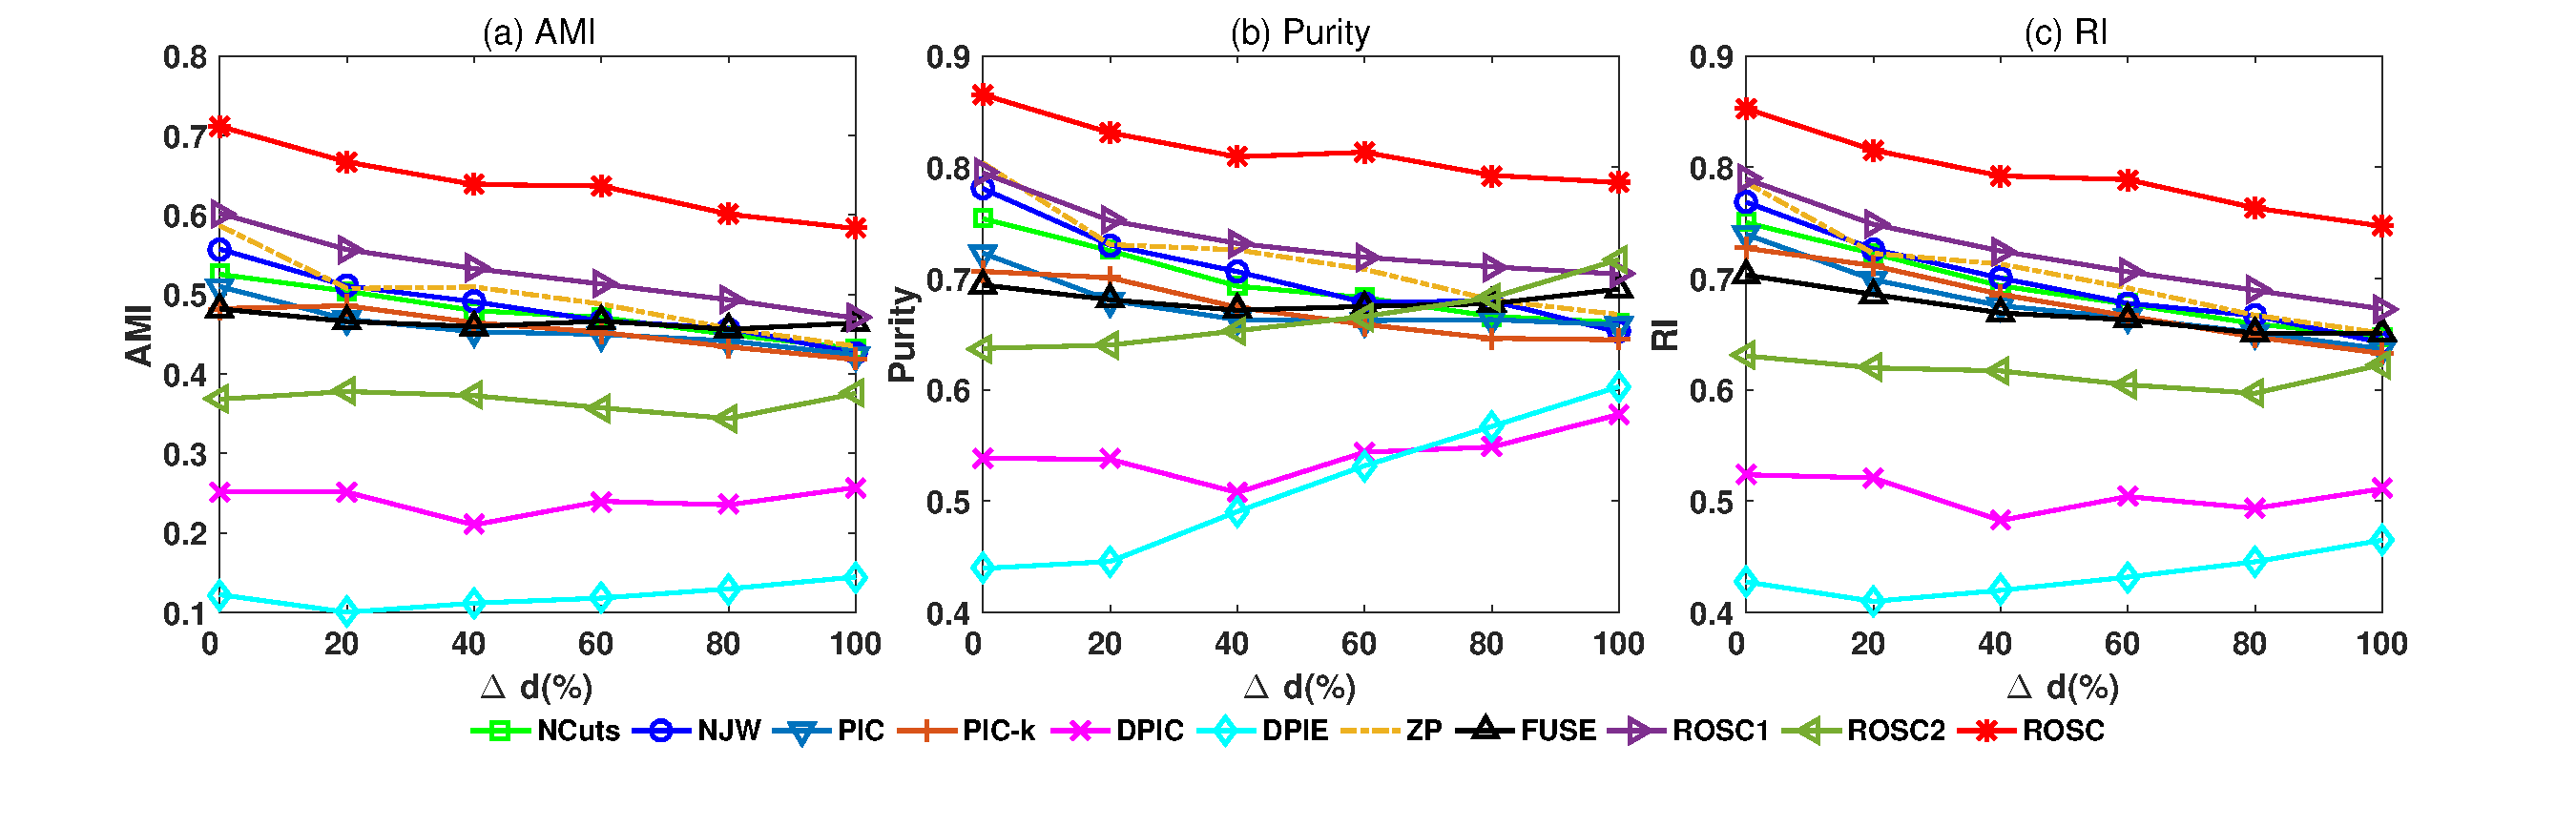
\includegraphics[width = 0.7\linewidth]{figure/syn1_d_1.eps}
%        \vspace{-0.5cm}
%        \caption{Clustering results with varying density on \textsc{Syn1}}
%        \label{figure:syn1_d}
%    \centering
%        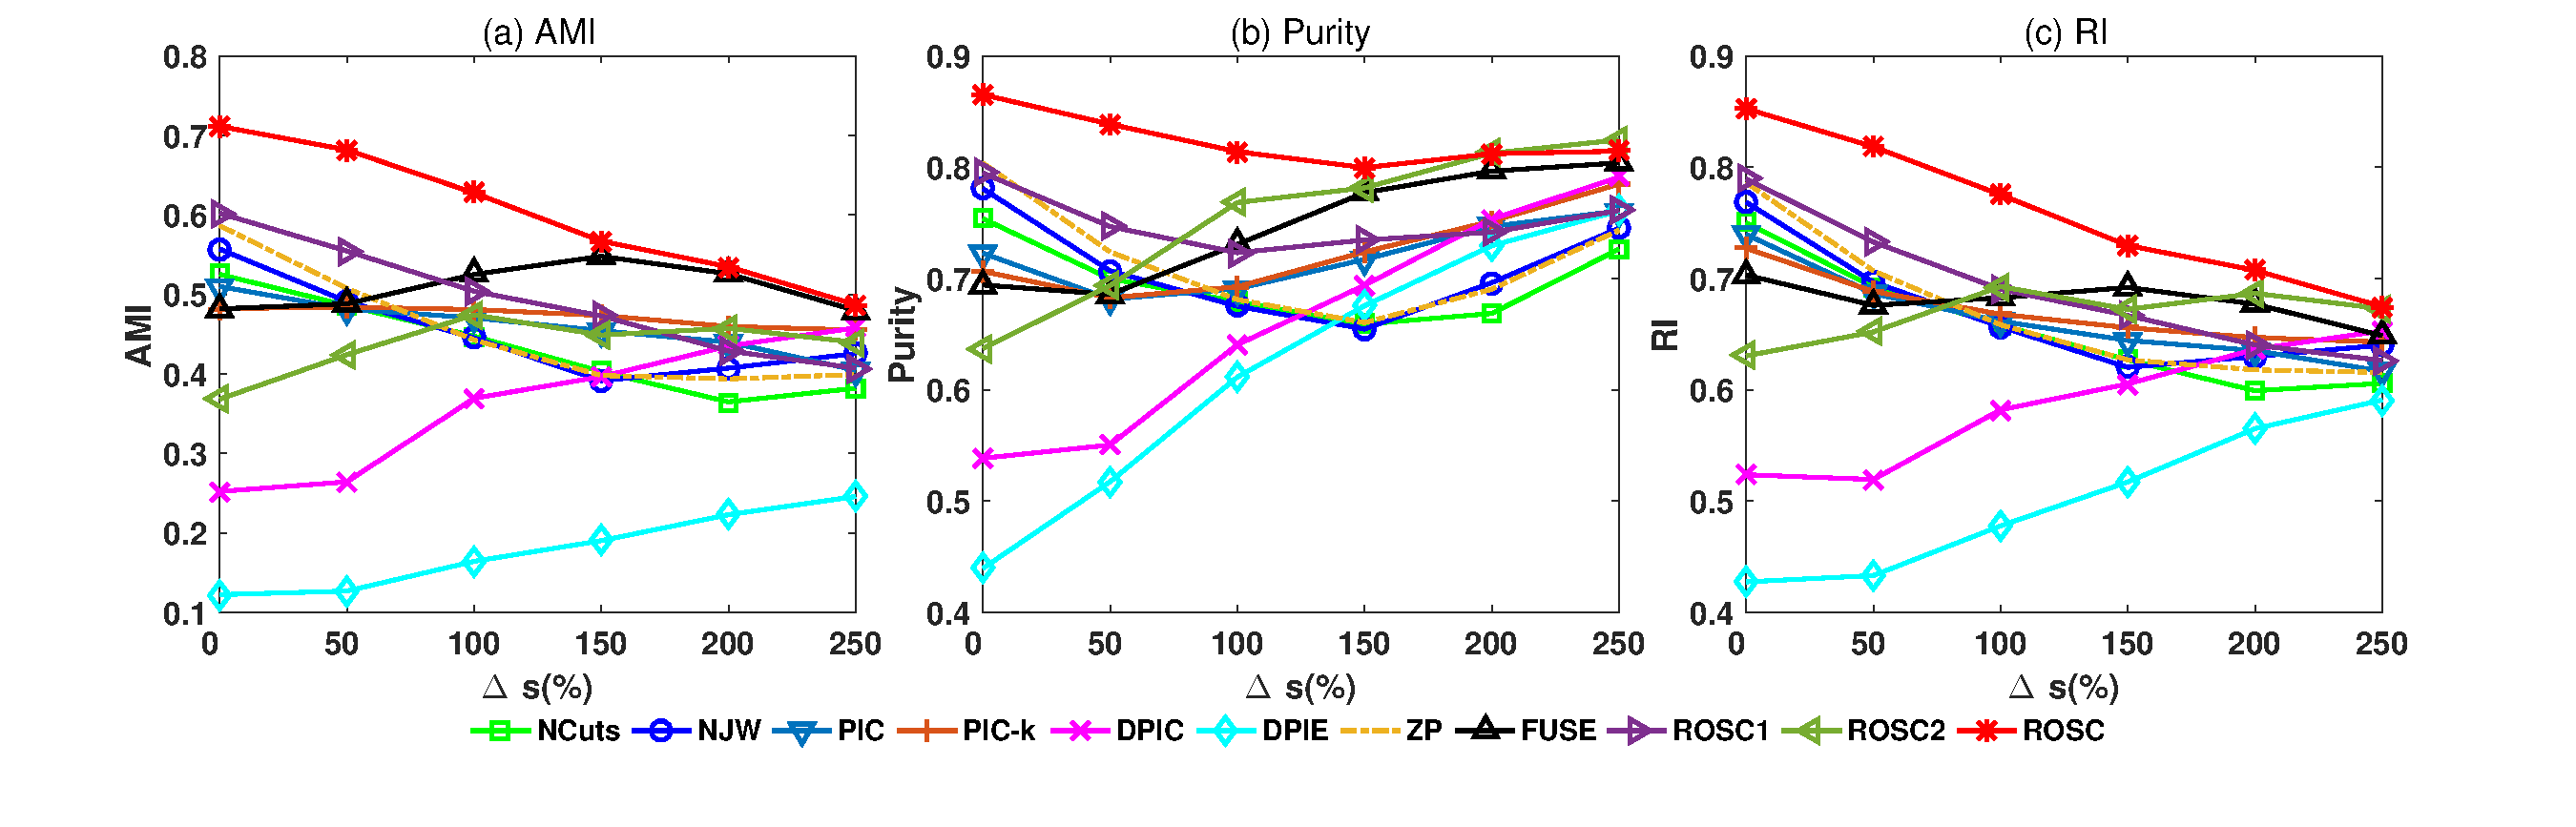
\includegraphics[width =0.7\linewidth]{figure/syn1_s_1.eps}
%        \vspace{-0.5cm}
%        \caption{Clustering results with varying size on \textsc{Syn1}}
%        \label{figure:syn1_s}
%%\end{figure*}
%%\begin{figure*}[!htbp]
    \centering
        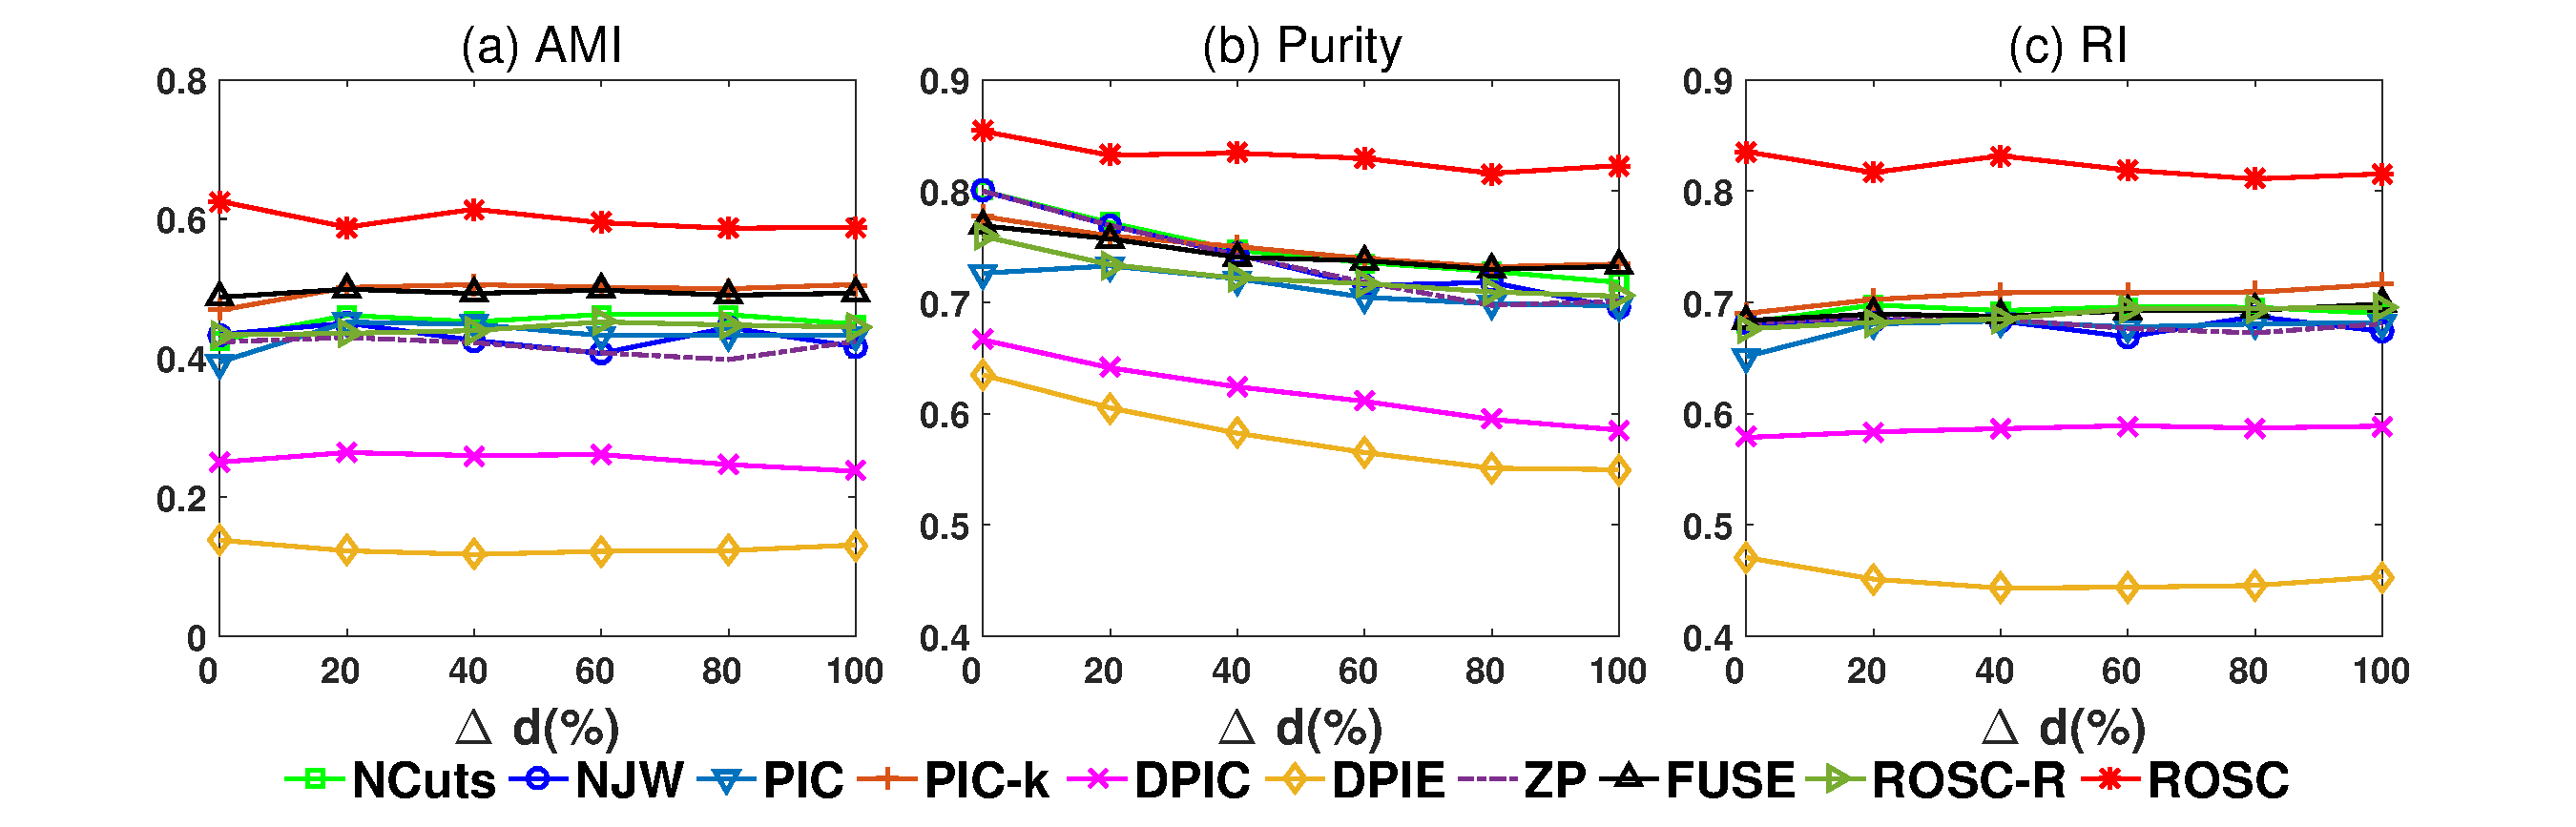
\includegraphics[width = 0.7\linewidth]{figure/syn2_d_1.eps}
        \vspace{-0.5cm}
        \caption{Performance scores of methods vs. varying blue cluster's density in \textsc{Syn1}}
        \label{figure:syn2_d}
    \centering
        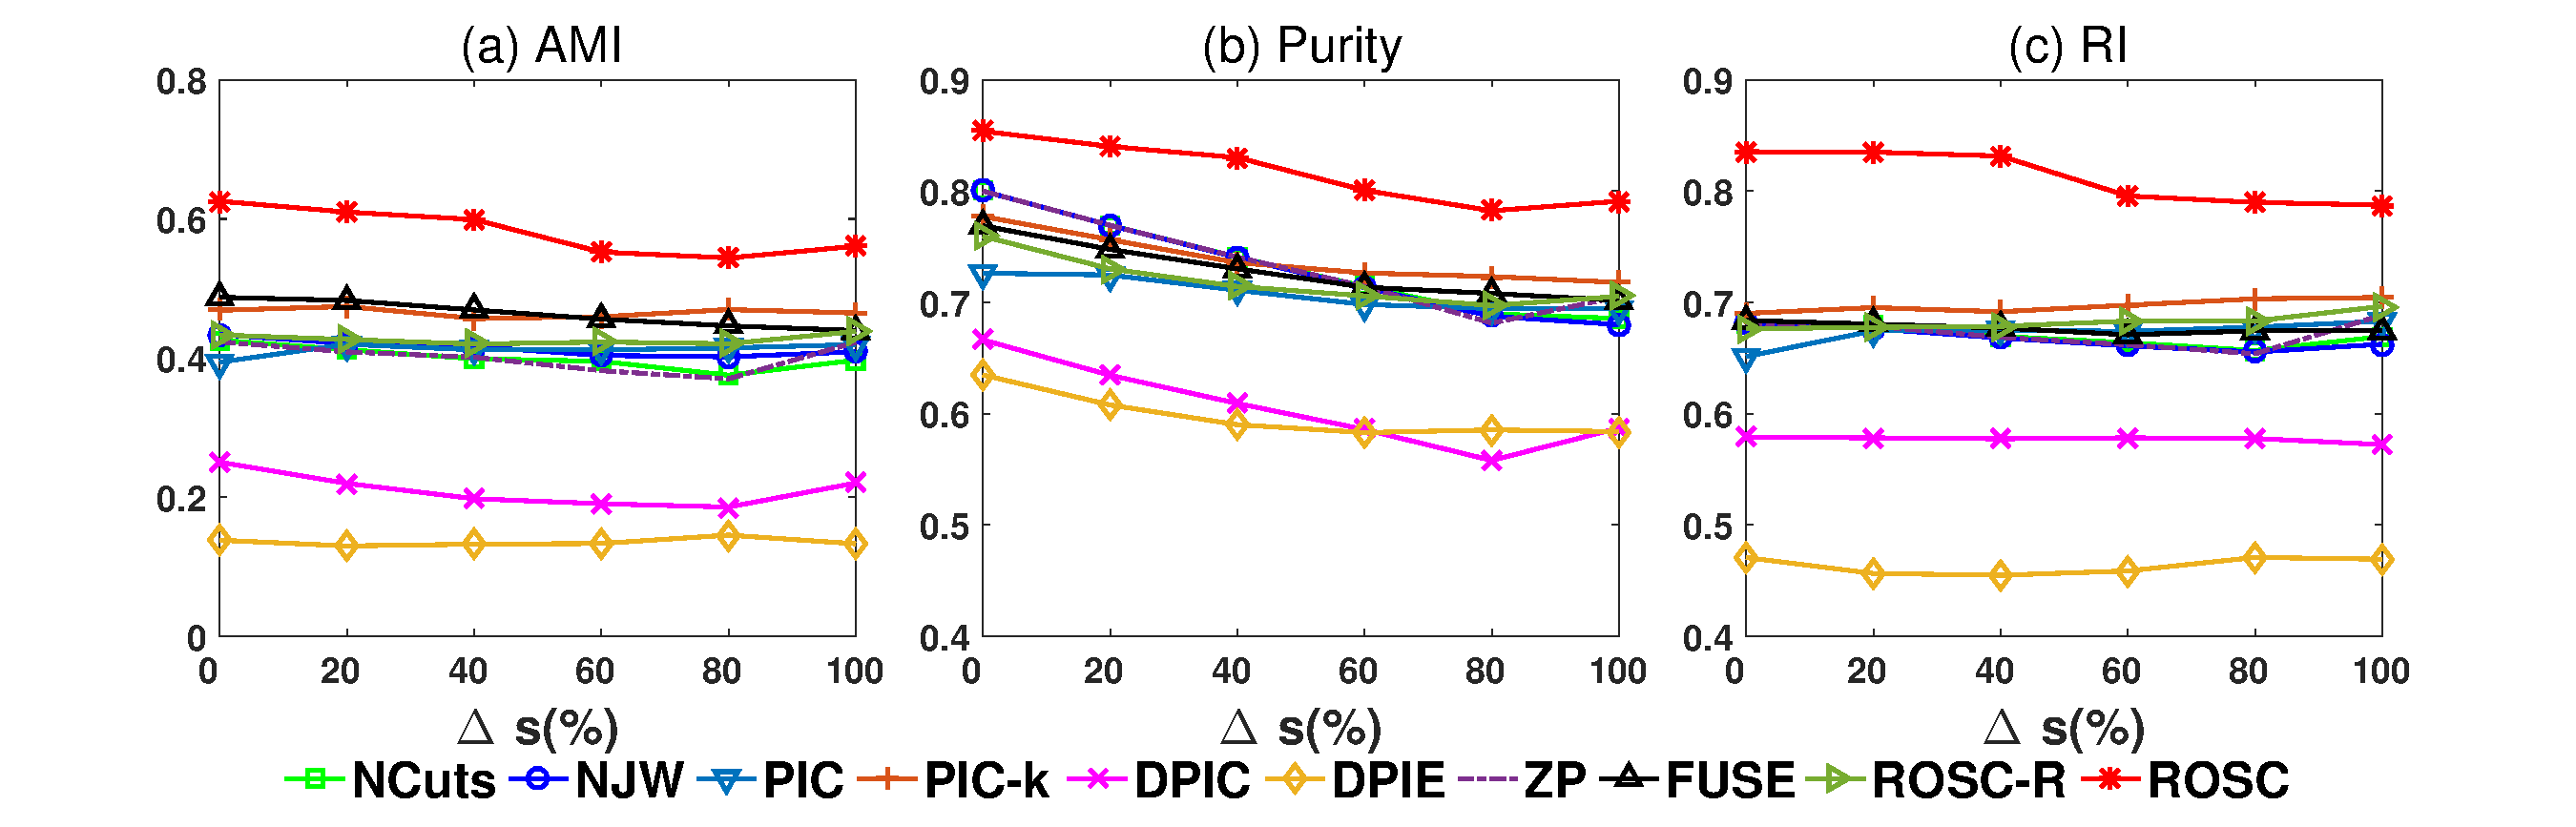
\includegraphics[width = 0.7\linewidth]{figure/syn2_s_1.eps}
        \vspace{-0.5cm}
        \caption{Performance scores of methods vs. varying blue cluster's size in \textsc{Syn1}}
        \label{figure:syn2_s}
%\end{figure*}
%\begin{figure*}[!htbp]
     \centering
        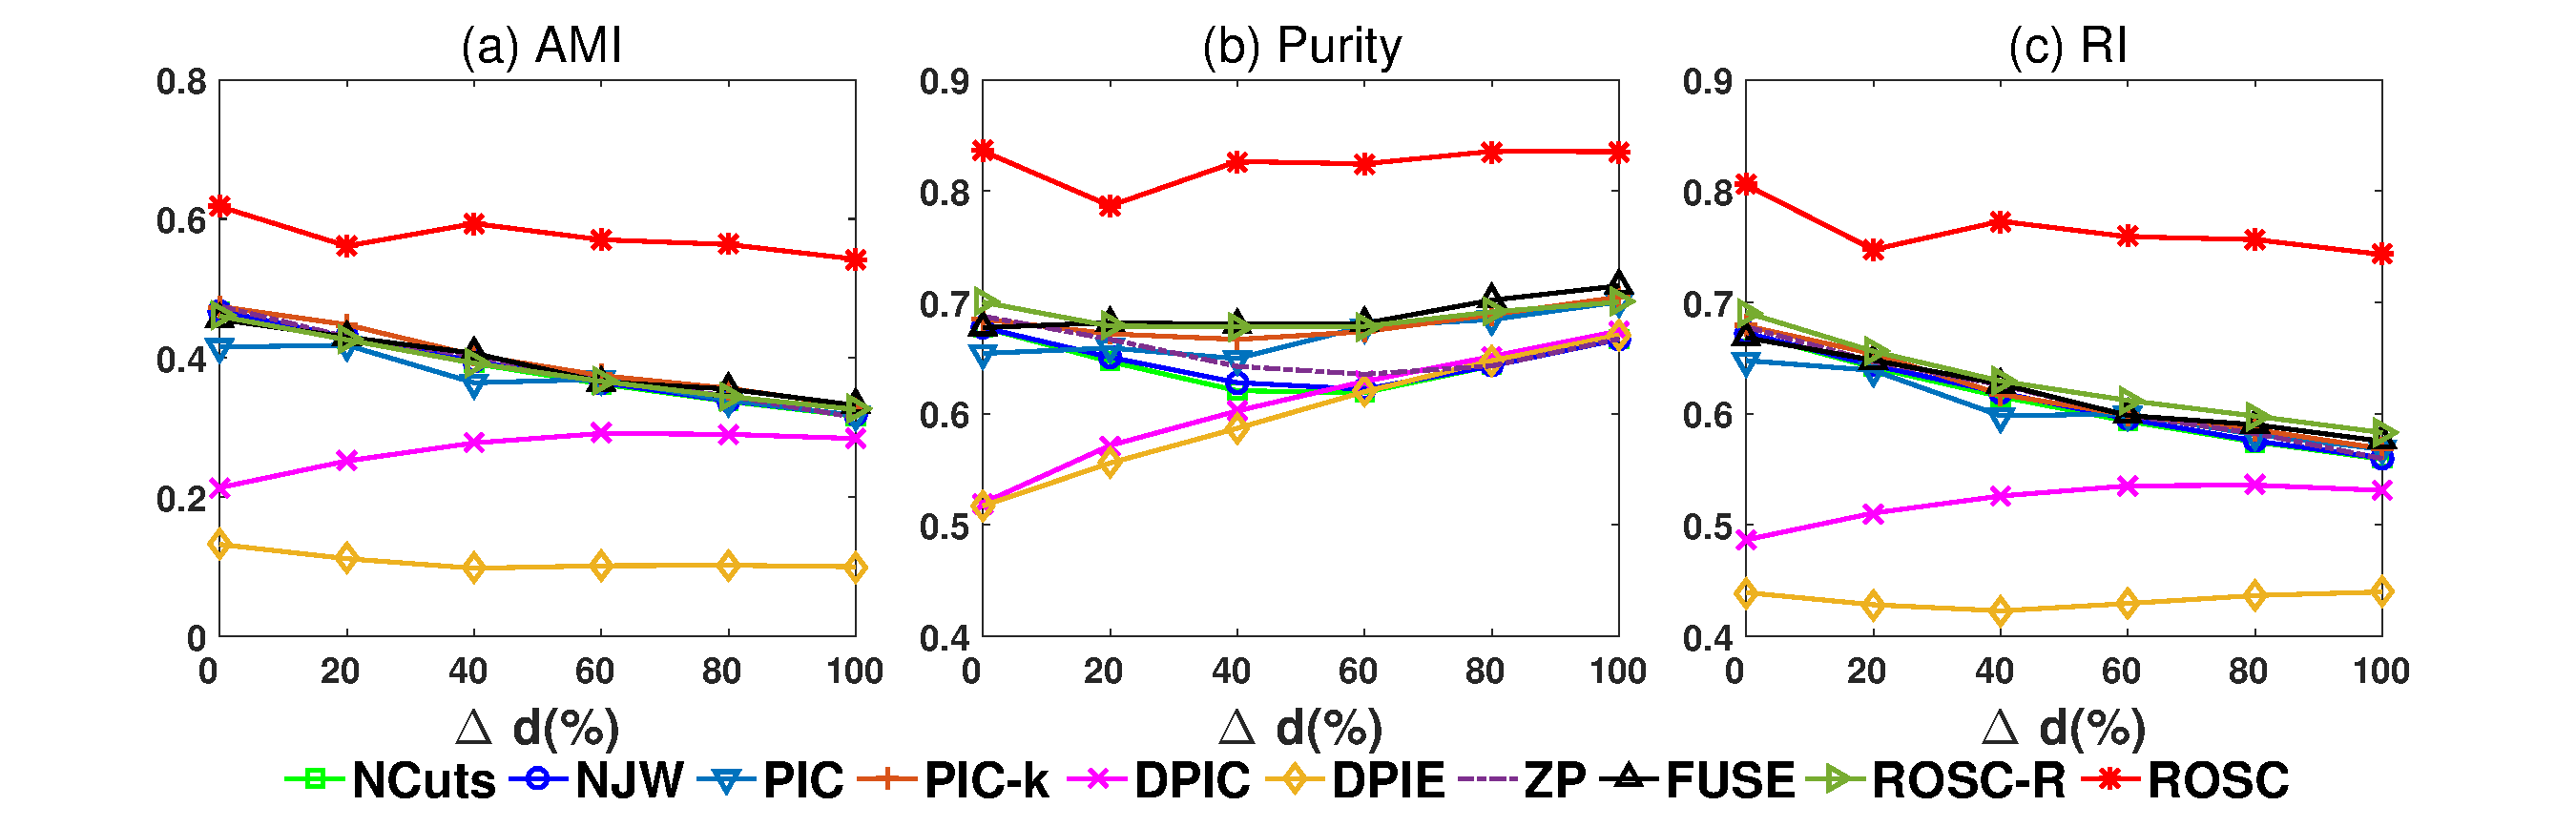
\includegraphics[width = 0.7\linewidth]{figure/syn3_d_1.eps}
        \vspace{-0.5cm}
        \caption{Performance scores of methods vs. varying green cluster's density in \textsc{Syn2}}
        \label{figure:syn3_d}
    \centering
        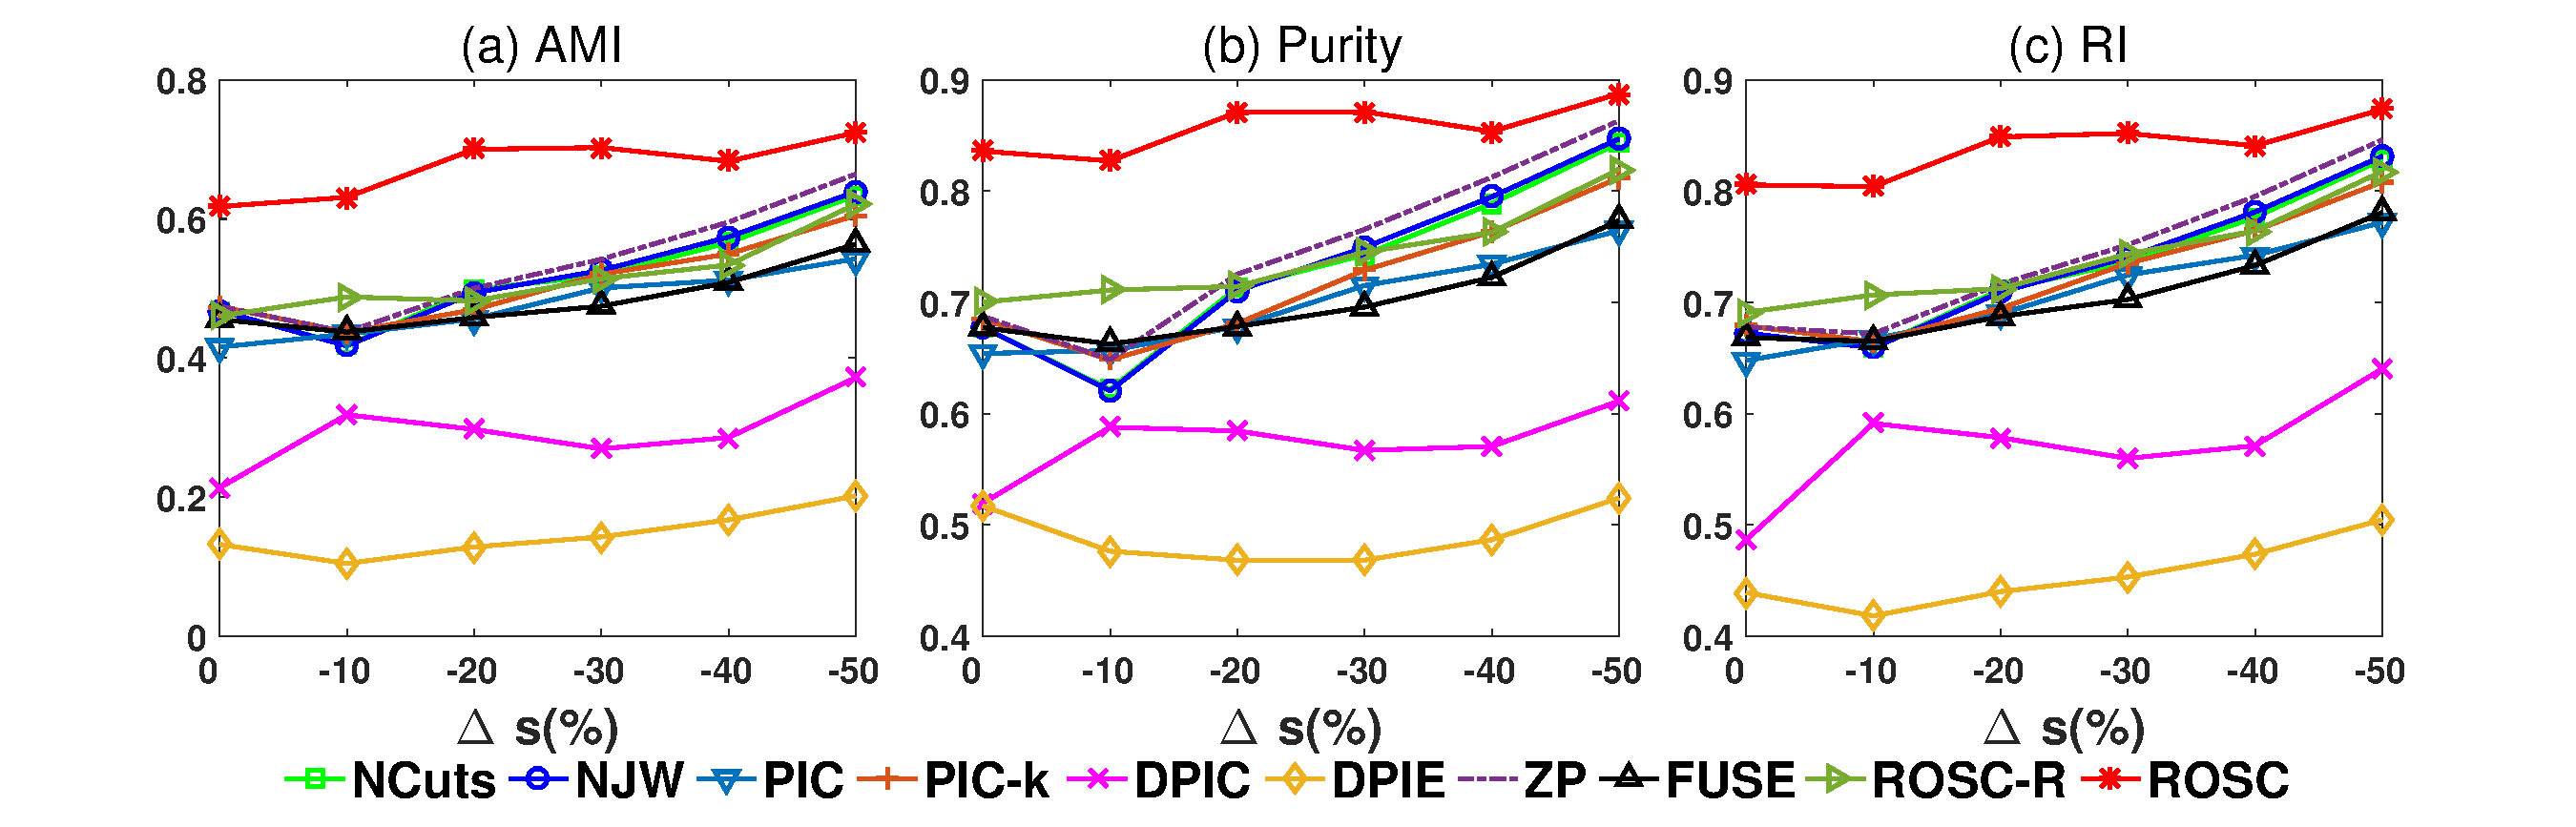
\includegraphics[width =0.7\linewidth]{figure/syn3_s_1.eps}
        \vspace{-0.5cm}
        \caption{Performance scores of methods vs. varying green cluster's size in \textsc{Syn2}}
        \label{figure:syn3_s}
\end{figure*}
}

\begin{figure}[!htbp]
        \centering
        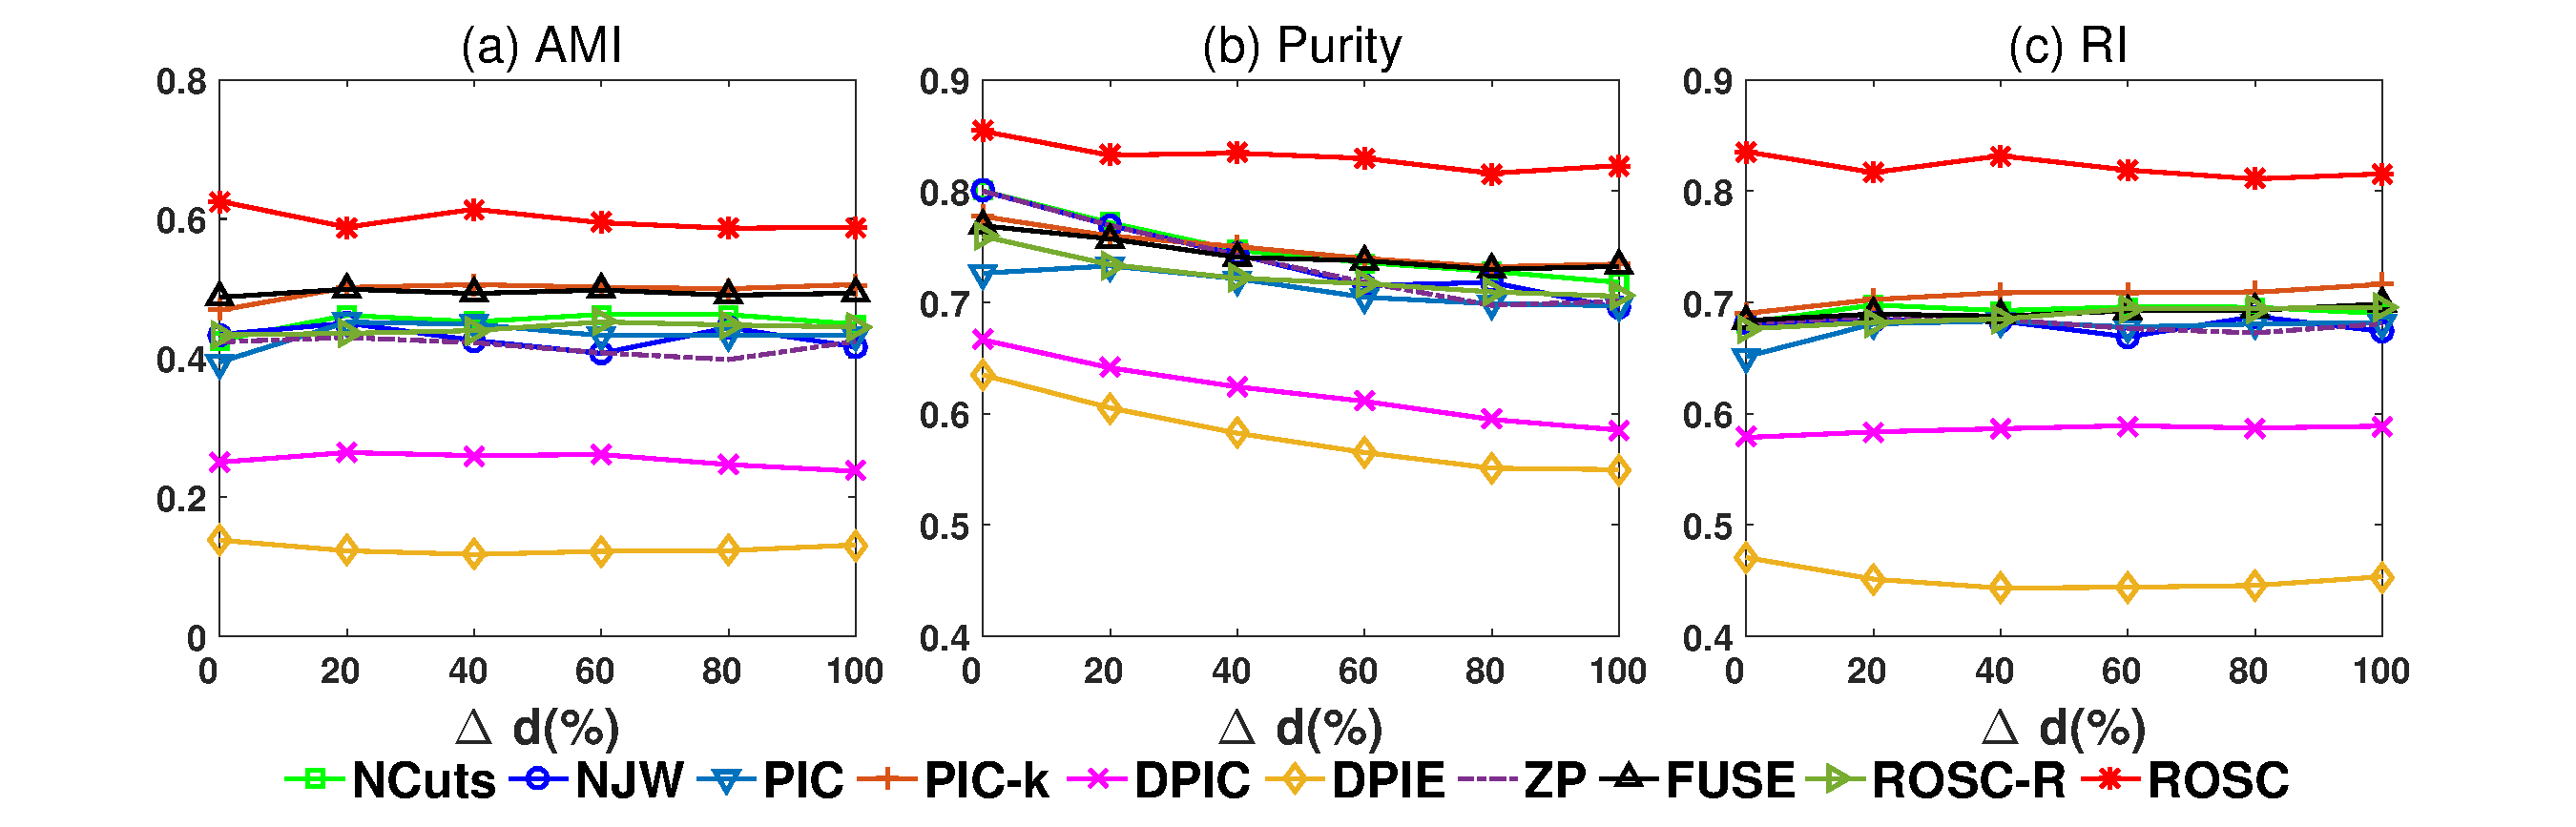
\includegraphics[width=0.5\textwidth]{figure/syn2_d_1.eps}
        \vspace{-0.5cm}
        \caption{Results vs. varying blue cluster's density in \textsc{Syn1}}
        \label{figure:syn2_d}
         \centering
         \vspace{0.2cm}
        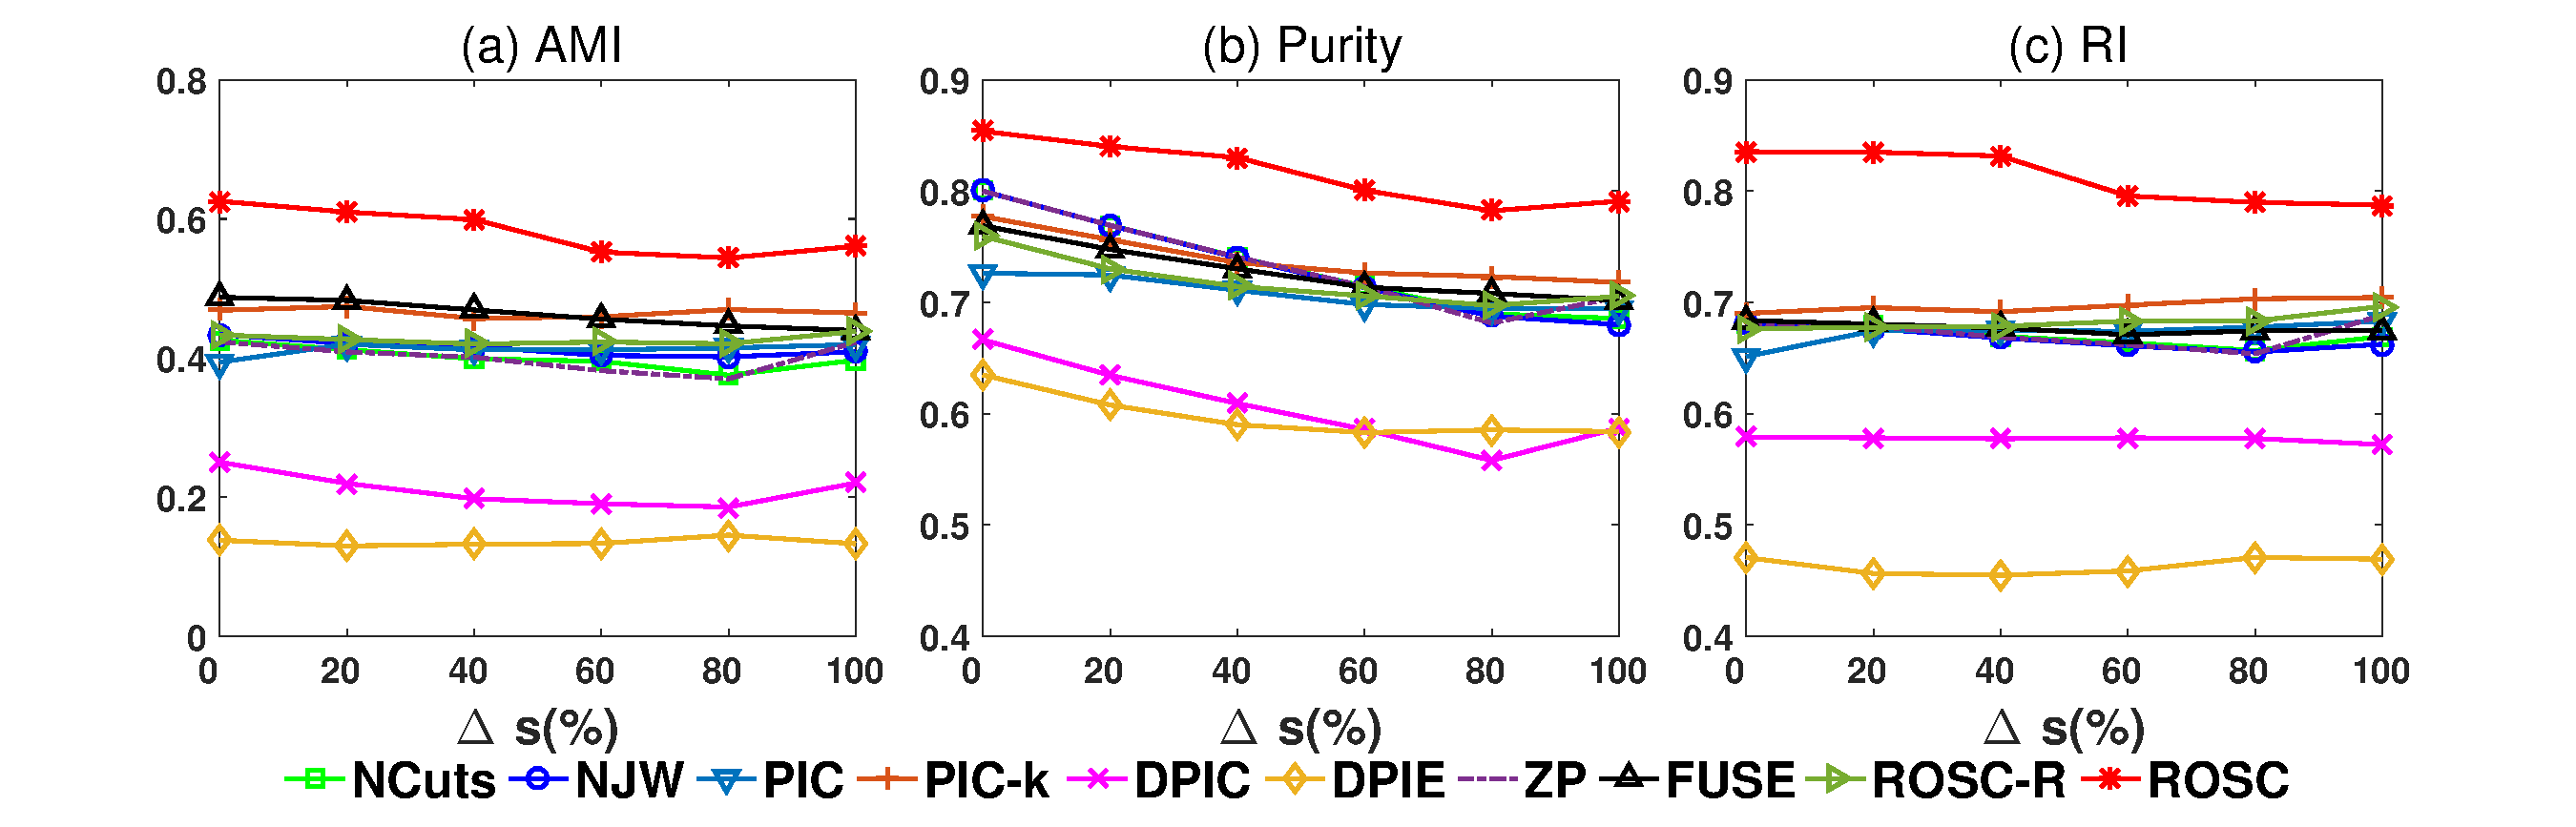
\includegraphics[width=0.5\textwidth]{figure/syn2_s_1.eps}
        \vspace{-0.5cm}
        \caption{Results vs. varying blue cluster's size in \textsc{Syn1}}
        \label{figure:syn2_s}
         \centering
         \vspace{0.2cm}
        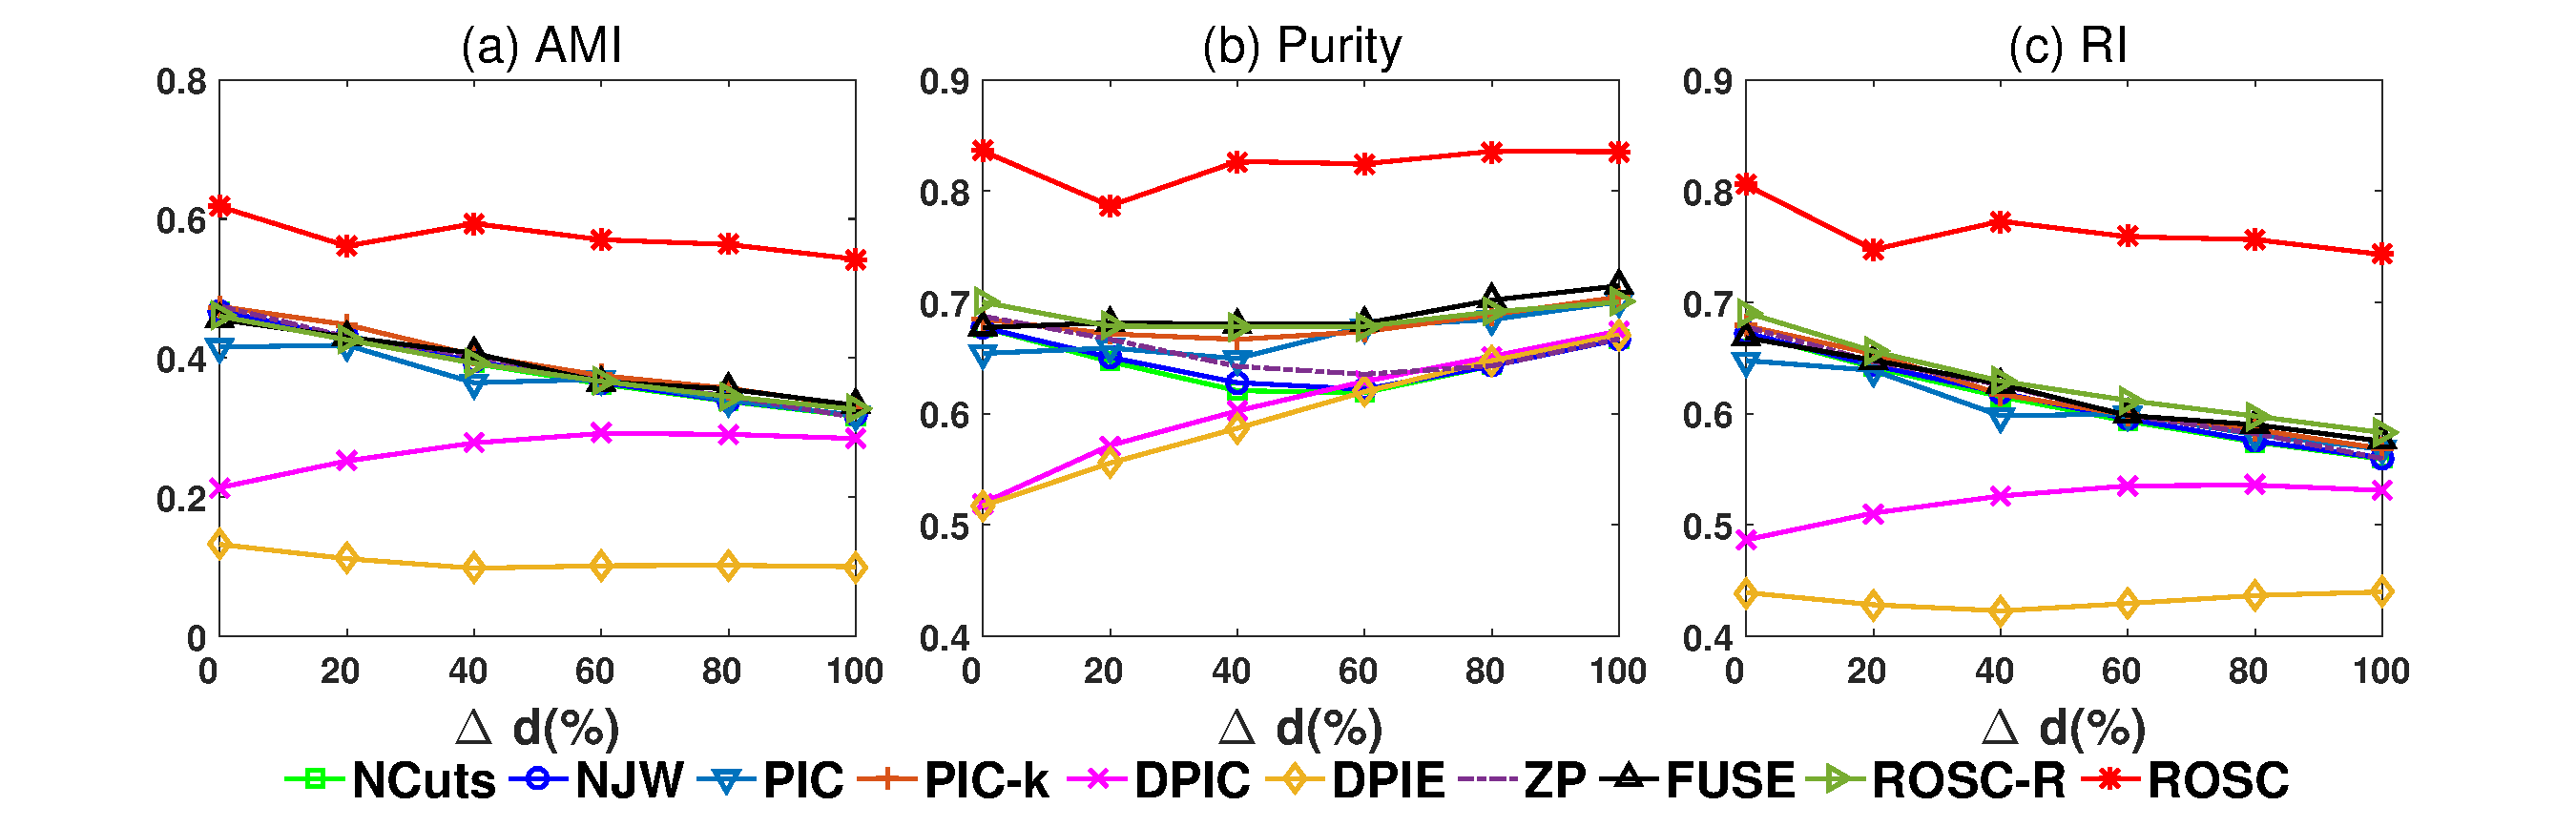
\includegraphics[width=0.5\textwidth]{figure/syn3_d_1.eps}
        \vspace{-0.5cm}
        \caption{Results vs. varying green cluster's density in \textsc{Syn2}}
        \label{figure:syn3_d}
         \centering
         \vspace{0.2cm}
        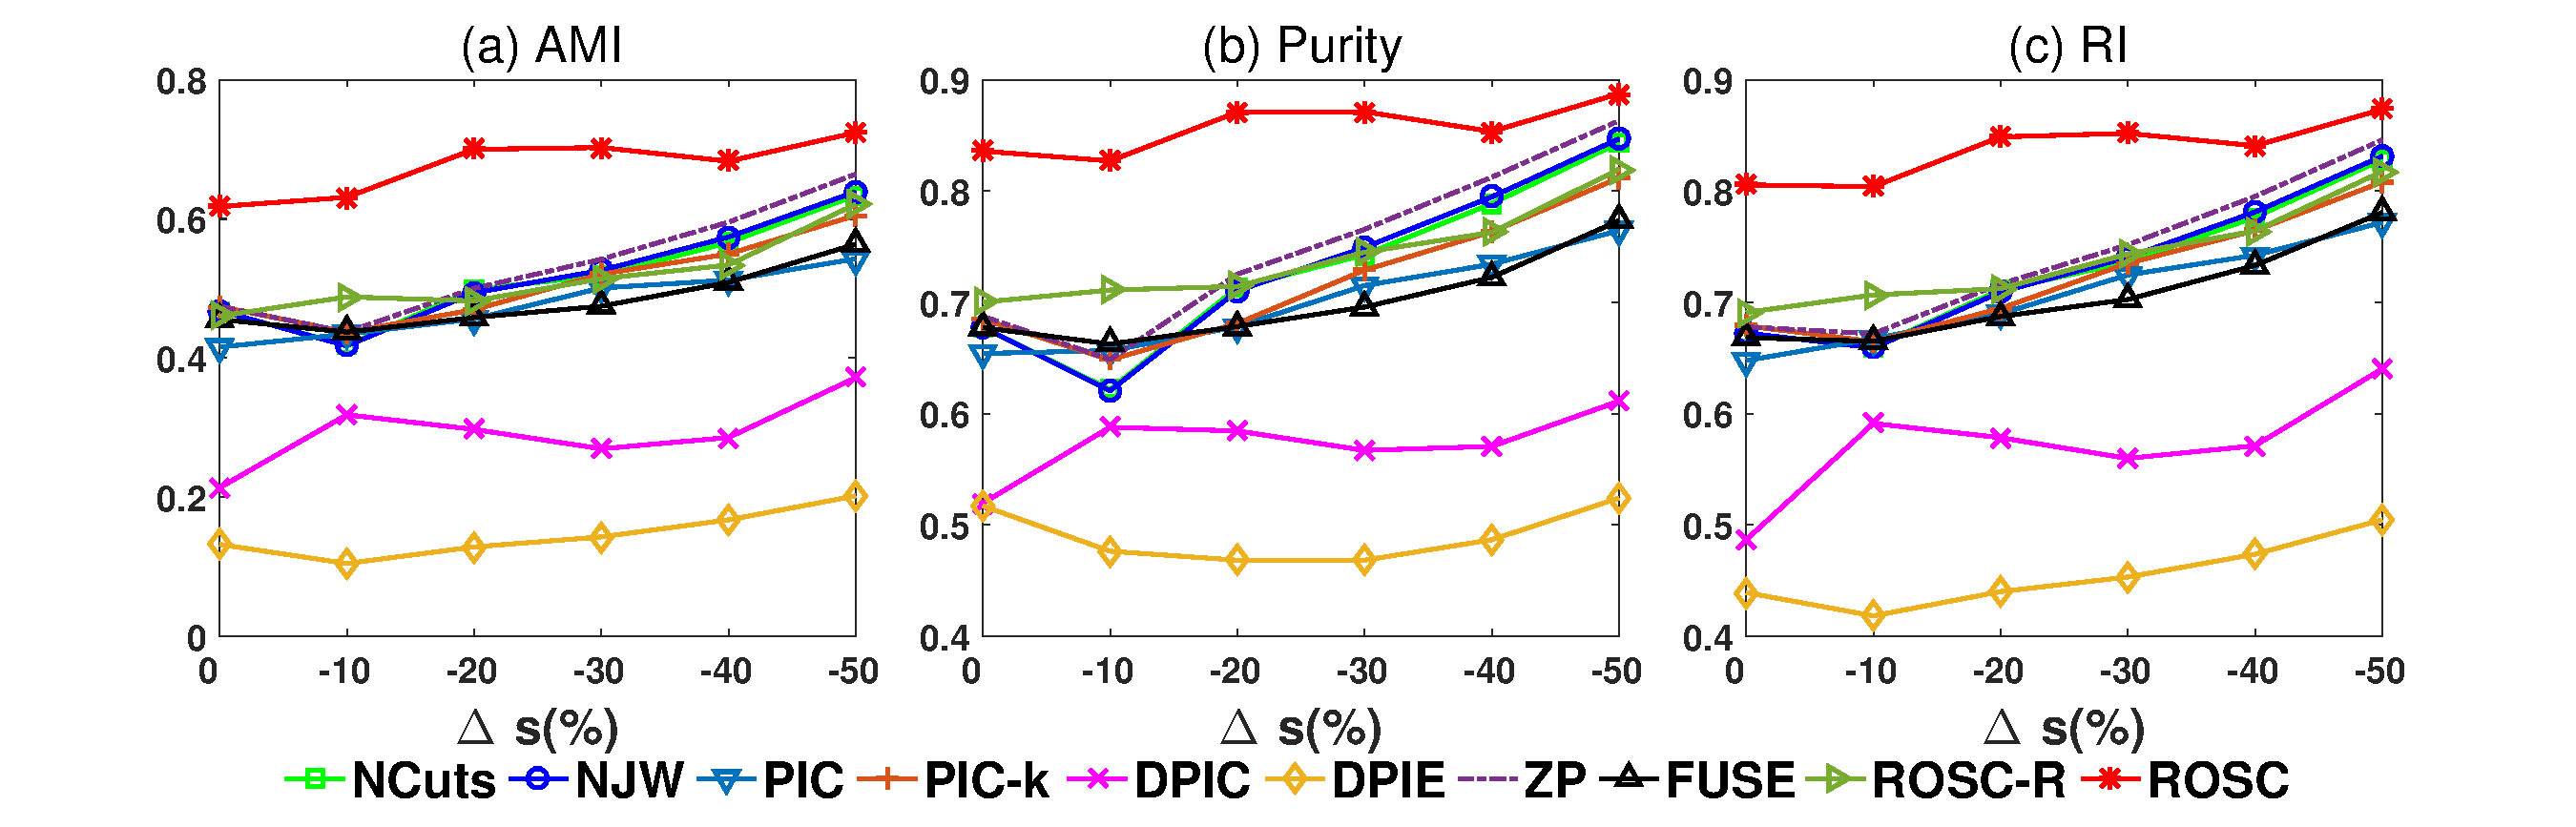
\includegraphics[width=0.5\textwidth]{figure/syn3_s_1.eps}
        \vspace{-0.5cm}
    \caption{Results vs. varying green cluster's size in \textsc{Syn2}}
     \label{figure:syn3_s}
     \vspace{-5mm}
\end{figure}


\comment{
From Fig.~\ref{figure:syn2}, ROSC performs well in identifying the annular cluster
while ZP correctly finds Gaussian distributed clusters and uniformly distributed clusters
with misclassification on a part of objects in the annular cluster.
}

\comment{
Fig.~\ref{figure:syn3}(a) depicts a dataset with three clusters.
One uniformly distributed cluster with 400 objects 
lays between two Gaussian distributed clusters with 100 objects each.
In this case, ROSC shows its huge advantage over all the baselines.
Compared with the second best results,
ROSC achieves $32\%$ increase in AMI, $12\%$ increase in purity and $24\%$ increase in RI.
It can almost correctly distinguish all the three clusters 
except misclassifying a few objects in the two Gaussian distributed clusters.
However, the baseline methods misclassify a great proportion of objects 
in the rectangular into the Gaussian distributed clusters.

The clustering result on the fourth dataset is described in Fig.~\ref{figure:syn4}.
The dataset includes two Gaussian distributed clusters and one half-ring cluster. 
Since two-end objects in the half ring are very close to the two Gaussian distributed clusters,
it is easy to misclassify them.
Although it is a difficult task,
our method ROSC can still achieve the best performance in all measures.
From Fig.~\ref{figure:syn4},
ROSC can correctly cluster one-end objects in the half ring while ZP misclassify objects in both the two ends. 
DPIC puts the two Gaussian distributed clusters into one cluster, leading to an even worse result.

Based on these synthetic datasets, we observe that 
ROSC outperforms baseline methods on three datasets and performs well on the second one,
which proves that ROSC is robust.
In comparison, other methods like ZP, 
even though it works best on the second dataset, 
it performs poorly on others.
Since ROSC fuses cluster-separation information in all the eigenvectors, removes the contained noise,
and applies the TKNN graph to rectify the similarity matrix,
the new matrix is more accurate in reflecting the true similarities between objects,
which leads to the robustness of ROSC.
However, the baseline methods does not correct
the inaccurate similarities in the original matrix, 
so they are unstable.


\begin{table*}[!htbp]
\centering
\caption{AMI comparison on synthetic datasets}
\label{table:ami_synthetic}
\resizebox{0.8\linewidth}{!}
{
\begin{tabular}{|c|c|c|c|c|c|c|c|c|c|c|} \hline
Dataset &NJW & NCuts & ZP & PIC & PIC-$k$ & DPIC & DPIE & FUSE & ROSC \\ \hline 
syn1 & $0.1877$ & $0.1863$ & $0.2687$ & $0.3108$ & $0.3279$ & $0.2030$ & $0.2340$ & $0.3692$ & $\bm{0.4384\ (1)}$ \\ \hline
syn2 & $0.8570$ & $0.8481$ & $\bm{0.8886}$ & $0.7726$ & $0.8265$ & $0.3346$ & $0.3829$ & $0.7834$ & $0.8631\ (2)$ \\ \hline
syn3 & $0.5295$ & $0.5310$ & $0.5452$ & $0.5003$ & $0.5849$ & $0.4235$ & $0.2990$ & $0.5636$ & $\bm{0.7743\ (1)}$ \\ \hline
syn3 & $0.5377$ & $0.5235$ & $0.5384$ & $0.5098$ & $0.5582$ & $0.4204$ & $0.1685$ & $0.5061$ & $\bm{0.6500\ (1)}$ \\ \hline
\end{tabular}
}
\end{table*}

\begin{table*}[!htbp]
\centering
\caption{Purity comparison on synthetic datasets}
\label{table:purity_synthetic}
\resizebox{0.8\linewidth}{!}
{
\begin{tabular}{|c|c|c|c|c|c|c|c|c|c|c|} \hline
Dataset &NJW & NCuts & ZP & PIC & PIC-$k$ & DPIC & DPIE & FUSE & ROSC \\ \hline 
syn1 & $0.7143$ & $0.7143$ & $0.7143$ & $0.7554$ & $0.7795$ & $0.7337$ & $0.7742$ & $0.7927$ & $\bm{0.8515\ (1)}$ \\ \hline
syn2 & $0.9138$ & $0.9138$ & $\bm{0.9277}$ & $0.8362$ & $0.8858$ & $0.5385$ & $0.5418$ & $0.8619$ & $0.9210\ (2)$ \\ \hline
syn3 & $0.8317$ & $0.8317$ & $0.8317$ & $0.8119$ & $0.8366$ & $0.7696$ & $0.7598$ & $0.8402$ & $\bm{0.9417\ (1)}$ \\ \hline
syn3 & $0.7712$ & $0.7550$ & $0.7725$ & $0.6998$ & $0.7330$ & $0.6789$ & $0.5328$ & $0.7169$ & $\bm{0.8226\ (1)}$ \\ \hline
\end{tabular}
}
\end{table*}

\begin{table*}[!htbp]
\centering
\caption{Rand index comparison on synthetic datasets}
\label{table:ri_synthetic}
\resizebox{0.8\linewidth}{!}
{
\begin{tabular}{|c|c|c|c|c|c|c|c|c|c|c|} \hline
Dataset &NJW & NCuts & ZP & PIC & PIC-$k$ & DPIC & DPIE & FUSE & ROSC \\ \hline 
syn1 & $0.5178$ & $0.5157$ & $0.5398$ & $0.5688$ & $0.5882$ & $0.5354$ & $0.5952$ & $0.5986$ & $\bm{0.7121\ (1)}$ \\ \hline
syn2 & $0.9543$ & $0.9519$ & $\bm{0.9630}$ & $0.9047$ & $0.9359$ & $0.5637$ & $0.5758$ & $0.9049$ & $0.9522\ (3)$ \\ \hline
syn3 & $0.6752$ & $0.6775$ & $0.7280$ & $0.6967$ & $0.7273$ & $0.6290$ & $0.6013$ & $0.7163$ & $\bm{0.9044\ (1)}$ \\ \hline
syn3 & $0.7358$ & $0.7232$ & $0.7368$ & $0.6875$ & $0.7145$ & $0.6510$ & $0.4464$ & $0.6998$ & $\bm{0.7919\ (1)}$ \\ \hline
\end{tabular}
}
\end{table*}
}

\noindent{\bf[Real datasets]}
We further evaluate the methods using 7 real datasets.
They are:
%\ngd\ (text documents from 20Newsgroup),
\mnist\ (hand-written digit images),
\coil\ (images),
\yale\ (facial images),
\isolet\ (speech, UCI repository),
\seg\ (images, UCI repository),
\yeast\ (biological data, UCI repository),
\glass\ (UCI repository).
Table~\ref{table:des_real} summarizes these datasets.
For each dataset, we show the number of objects, the number of dimensions, and the number of clusters.
Also, to show whether a dataset is multi-scale or not, we measure the {\it size} and {\it density} of each
gold-standard cluster in each dataset. 
Specifically, for each cluster, we find the largest distance of any object-pair of the cluster. 
This distance is taken as the {\it diameter} of cluster, reflecting how big in size the cluster is.
Moreover, for each cluster, we find the average distance, $\rho$, of all object-pairs of the cluster. 
Then, we use $1/\rho$ as a measure of density. These cluster sizes and densities are shown in
bar graphs in Table~\ref{table:des_real}.
%\footnote{We do not show the sizes and densities of the clusters
%for the {\it 20ngD} dataset because the objects are text documents with extremely sparse and high dimensions.}.
The sizes (densities) shown are all normalized by the size (density) of the biggest (densest) cluster
of the corresponding dataset to the range [0, 1].
Intuitively, the more variations in the bars of a graph indicate the more multi-scale the corresponding
dataset is.
 
From Table~\ref{table:des_real}, we see the dataset \coil\ is highly multi-scale. 
For example, cluster 2 (the largest cluster) is $5.6$ times larger than cluster 15 (the smallest cluster).
However, cluster 15 is $5.9$ times denser than cluster 2.
The dataset \glass\ is moderately multi-scale, and \yale\ is relatively 
uniform.
The dataset \seg\ is interesting because it has one very big and sparse cluster
(cluster 3); the other 6 clusters are quite uniform.

%To further study ROSC, 
%we also conduct experiments on 8 real datasets.
%\emph{20ngD}, \emph{MNIST0127} and \emph{Yale\_5\textsc{class}} are extracted from the text dataset 20Newsgroups,
%the hand-written digits dataset MNIST 
%and the face image dataset Yale respectively.
%All these original datasets as well as the image dataset \emph{COIL20} are publicly available.
%\emph{isolet\_5\textsc{class}}, \emph{seg\_7\textsc{class}} and \emph{Yeast\_4\textsc{class}} are extracted from 
%Isolet, Image segmentation and Yeast datasets
%in the UCI machine learning repository,
%where \emph{glass} can also be found.
%Details on these datasets are summarized in Table~\ref{table:des_real}.
%For all the datasets, a preprocessing step is required to normalize attributes before computing the similarity matrix.
\begin{table*}[!htbp]
\centering
\resizebox{0.9\linewidth}{!}
{
\begin{tabular}{|c|c|c|c|c|c|} \hline
Dataset & \#objects & \#dimensions & \#clusters & size & density\\ \hline 
%20ngD & $800$ & $26214$ & $4$ & - & - \\ \hline
COIL20 &$1440$ & $1024$ & $20$ & \begin{minipage}{0.2\textwidth}\centering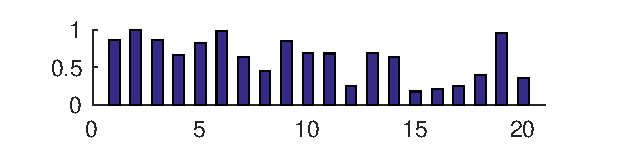
\includegraphics[height=8mm]{figure/COIL20_size.eps}\end{minipage} & \begin{minipage}{0.2\textwidth}\centering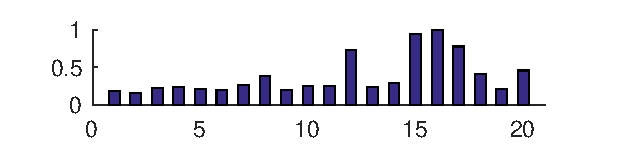
\includegraphics[height=8mm]{figure/COIL20_den.eps}\end{minipage} \\ \hline
seg\_7\textsc{class} &$210$ & $19$ & $7$ & \begin{minipage}{0.2\textwidth}\centering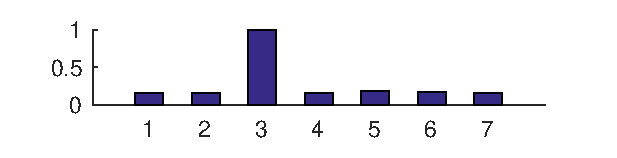
\includegraphics[height=8mm]{figure/seg_size.eps}\end{minipage} & \begin{minipage}{0.2\textwidth}\centering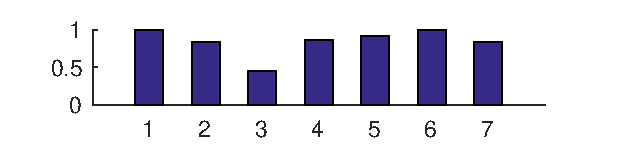
\includegraphics[height=8mm]{figure/seg_den.eps}\end{minipage} \\ \hline
glass &$214$ & $9$ & $6$  & \begin{minipage}{0.2\textwidth}\centering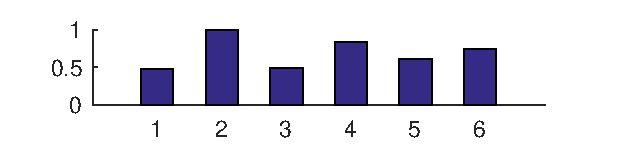
\includegraphics[height=8mm]{figure/glass_size.eps}\end{minipage} & \begin{minipage}{0.2\textwidth}\centering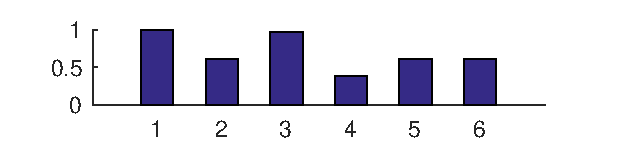
\includegraphics[height=8mm]{figure/glass_den.eps}\end{minipage} \\ \hline
MNIST0127 & $1666$ & $784$ & $4$ & \begin{minipage}{0.2\textwidth}\centering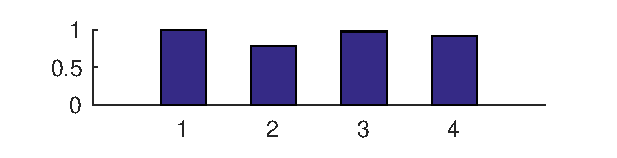
\includegraphics[height=8mm]{figure/mnist_size.eps}\end{minipage} & \begin{minipage}{0.2\textwidth}\centering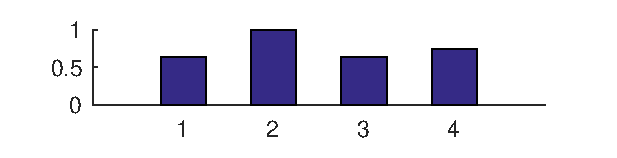
\includegraphics[height=8mm]{figure/mnist_den.eps}\end{minipage} \\ \hline
isolet\_5\textsc{class}&$300$ & $617$ & $5$ & \begin{minipage}{0.2\textwidth}\centering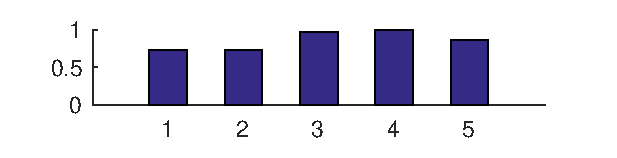
\includegraphics[height=8mm]{figure/isolet_size.eps}\end{minipage} & \begin{minipage}{0.2\textwidth}\centering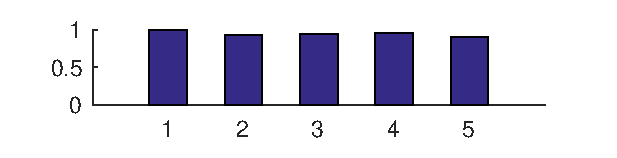
\includegraphics[height=8mm]{figure/isolet_den.eps}\end{minipage}\\ \hline
Yeast\_4\textsc{class}&$1299$ & $8$ & $4$ & \begin{minipage}{0.2\textwidth}\centering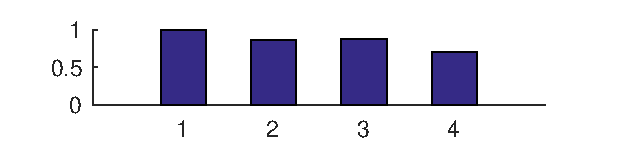
\includegraphics[height=8mm]{figure/yeast_size.eps}\end{minipage} & \begin{minipage}{0.2\textwidth}\centering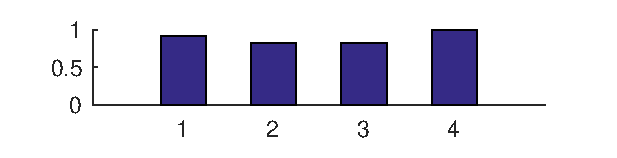
\includegraphics[height=8mm]{figure/yeast_den.eps}\end{minipage}\\ \hline
Yale\_5\textsc{class}&$55$ & $1024$ & $5$ & \begin{minipage}{0.2\textwidth}\centering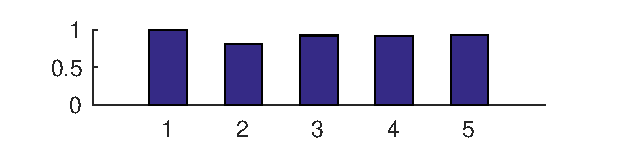
\includegraphics[height=8mm]{figure/yale_size.eps}\end{minipage} & \begin{minipage}{0.2\textwidth}\centering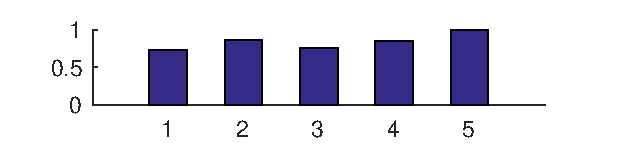
\includegraphics[height=8mm]{figure/yale_den.eps}\end{minipage} \\ \hline
\end{tabular}
}
\caption{Statistics of 7 real datasets}
\label{table:des_real}
\end{table*}

%\begin{minipage}[t]{0.85\textwidth}\lipsum[1]\end{minipage}

Tables~\ref{table:purity_real},~\ref{table:ami_real} and~\ref{table:ri_real} 
show the purity, AMI, and RI scores of the 10 methods when they are applied to the 7 real datasets.
Each row in the table corresponds to a (measure, dataset) combination --- or a contest
among the 10 methods. There are thus 21 (3 measures $\times$ 7 datasets) contests.
For each contest, the winner's score is shown in bold type.
For ROSC, its ranking in each contest is given in the bracket next to its score. 
The performance of a method can be judged by the column under the method spanning the three
tables. 
%In particular, the more bold-type numbers in a column indicates a better performance of a method.
From the tables, we make several observations:

(O1): Among the 21 contests, standard spectral clustering methods (NJW, NCuts) win only 2 times (AMI-\glass-NJW and AMI-\isolet-NJW).
PI-based methods (PIC, PIC-$k$, DPIC, DPIE) also win only 2 times
(purity-\isolet-DPIE and RI-\isolet-DPIE).
These two categories of methods, which are not designed to specifically handle
multi-scale data, are generally not outstanding. 

(O2): The multi-scale-data-oriented methods (ZP, FUSE) win 4 times. In fact, if we take away 
ROSC, then (ZP, FUSE) win 14 times of the 21 contests. They are thus fairly effective in clustering
multi-scale data. 
However, with a head-to-head comparison between ZP and FUSE, we see that 
%they split the 24 contests, with each winning 12 times.
among the 21 contests, ZP wins 9 times while FUSE wins 12 times. 
In some cases, there are big gaps in their performance scores.
For example, for the contest (AMI-\coil), ZP beats FUSE 0.5702 to 0.4448;
for (AMI-\yale), FUSE outscores ZP 0.3495 to 0.2788.
There is also a case (AMI-\isolet) in which FUSE (0.6516) loses significantly to the basic NJW method (0.7595).
We thus see that although ZP and FUSE generally perform well for multi-scale data, they are not very
robust in providing consistently good performances across the datasets. 

(O3): ROSC is winner 12 times and is first runner-up 6 times. Moreover, for those cases that ROSC does
not win, its score is very close to that of the winner.  
For example, ROSC ranks 4th in (RI-\isolet). Its score (0.9001), however, is quite close to that of
the winner DPIE (0.9123).
We thus see that ROSC is generally the best performer among all the 10 methods and it is very robust
across the 7 datasets tested. 

(O4): For \coil, ROSC outperforms other methods by very wide margins.
For example, in terms of purity, ROSC scores 0.9398, which is much better than
NJW (0.4115), DPIE (0.3496), and FUSE (0.4177).
From Table~\ref{table:des_real}, we see that \coil\ is highly multi-scale. 
The results thus highlight the ability of ROSC in clustering multi-scale data.
From the cluster size distribution, we see that there are clusters in \coil\ that are much bigger
than others. Objects in these big clusters can thus be very distant from each other and hence their
feature similarities are small.
Their correlations are alternatively captured by ROSC 
using the TKNN graph and the derived reachability matrix.
To see the effectiveness  of this approach, 
we compare the scores of ROSC against those of ROSC-R, which does not use the reachability matrix
to regularize $Z$. 
From Tables~\ref{table:purity_real}, \ref{table:ami_real}, \ref{table:ri_real}, we see big differences in
the scores of ROSC and ROSC-R for the rows of \coil. 
This verifies the importance of the TKNN graph in regularizing $Z$.

%
%
%\noindent{\small$\bullet$}
%The standard spectral clustering method NJW
%outperforms other comparison methods only in AMI on 
%datasets \emph{glass} and \emph{isolet\_5\textsc{class}}.
%
%\noindent{\small$\bullet$}
%Based on the results of PIC and PIC-\emph{k},
%simply using more pseudo-eigenvectors without 
%redundancy and noise reduction brings marginal benefit.
%
%\noindent{\small$\bullet$}
%Although DPIC and DPIE reduce redundancy by
%generating orthogonal and diverse pseudo-eigenvectors respectively,
%the contained noise finally leads to disastrous results.
%
%\noindent{\small$\bullet$}
%Both ZP and FUSE
%perform well in some cases.
%However,
%they lack the ability to rectify ineffective 
%similarities in the raw similarity matrix,
%leading to their unfavorable performance in other cases.
%
%\noindent{\small$\bullet$}
%With both redundancy and noise reduction in pseudo-eigenvectors,
%ROSC1 reserves the efficacy of effective similarities in the raw similarity matrix.
%So it outperforms the standard spectral clustering methods and PI based methods in most cases.
%However, compared with ROSC, it lacks the ability to rectify the ineffective similarities, 
%which lowers its robustness. 
%
%\noindent{\small$\bullet$}
%ROSC2 performs very well
%only on \emph{COIL20}. 
%In other cases, 
%using only the TKNN graph is insufficient 
%to ensure desiring clustering results.
%
%\noindent{\small$\bullet$}
%Compared with other methods,
%ROSC is always among the best ones with regard to all the three measures on all the datasets.
%It applies the TKNN graph to rectify the raw similarity matrix with the integration of noise reduction in pseudo-eigenvectors.
%A new similarity matrix is then constructed that reserves the efficacy of effective similarities and rectifies the ineffective ones in the raw similarity matrix,
%leading to the robustness of ROSC.
\comment{
We observe that ROSC takes the first place for three times.
In other cases, although it does not perform the best,
the gap with the best result is very small.
However, when ROSC performs the best, ROSC greatly outperforms all other methods,
e.g., ROSC achieves $0.9682$ on COIL20,
but the value of the second best method ZP is only $0.5702$.
The comparison on purity is shown in Table~\ref{table:purity_real}.
ROSC takes the first place for five times and the second for three times.
Experimental results on RI in
Table~\ref{table:ri_real} shows an even better result that ROSC takes the lead on 7 datasets.
All these results prove that ROSC is indeed robust.
In comparison, all the baseline methods are unstable. 
For example, FUSE performs very well on Yeast, but it works poorly on isolet\_5CLASS;
DPIE can achieve good result on isolet\_5CLASS, however, it fails on 20ngD.


The robustness of ROSC stems from its ability in 
retaining accurate similarities and correcting inaccurate ones. 
After rectification, object relations will be well reflected in the rectified similarity matrix,
which improves the clustering performance.
In the cases that inaccurate similarities may not be rectified, 
since ROSC reserves the original accurate similarities,
its performance will not be weaken.
}


\begin{table*}[!htbp]
%\end{table*}

%\begin{table*}[!htbp]
\centering
\resizebox{0.85\linewidth}{!}
{
\begin{tabular}{|c||c|c||c|c|c|c||c|c||c|c|} \hline
Dataset &NJW & NCuts  & PIC & PIC-$k$ & DPIC & DPIE & ZP & FUSE & ROSC-R & ROSC \\ \hline 
%20ngD & $0.4570$ & $0.4750$  & $0.4891$ & $0.4858$ & $0.3406$ & $0.3074$ & $0.5075$ & $0.4672$ & $0.5029$ & $\bm{0.5076\ (1)}$ \\ \hline
COIL20 &$0.4115$ & $0.3926$  & $0.2801$ & $0.2801$ & $0.2361$ & $0.3496$ & $0.5028$ & $0.4177$ & $0.4715$ & $\bm{0.9398\ (1)}$ \\ \hline
seg\_7\textsc{class} &$0.5608$ & $0.5403$  & $0.3483$ & $0.3566$ & $0.3000$ & $0.4756$ & $0.5143$ & $0.5912$ & $0.6209$ & $\bm{0.6636\ (1)}$ \\ \hline
%ecoli &$0.5338$ & $0.5365$ & $0.5339$ & $0.4366$ & $0.4814$ & $0.2073$ & $0.4325$ & $0.4550$ & $0.4770$ \\ \hline
glass &$0.5234$ & $0.5187$  & $0.4976$ & $0.5029$ & $0.5245$ & $0.5158$ & $0.5374$ & $0.5390$ &$0.5748$ & $\bm{0.5760\ (1)}$ \\ \hline
MNIST0127 & $0.5066$ & $0.4970$  & $0.4975$ & $0.4924$ & $0.5898$ & $0.4395$ & $0.5066$ & $0.6436$ & $0.6649$ & $\bm{0.6666\ (1)}$ \\ \hline
isolet\_5\textsc{class}&$0.8120$ & $0.7967$  & $0.5863$ & $0.5867$ & $0.3033$ & $\bm{0.8572}$ & $0.7767$ & $0.7825$ & $0.8495$ & $0.8179\ (3)$ \\ \hline
%statlog &$0.6571$ & $0.6590$ & $\bm{0.6882}$ & $0.5465$ & $0.6052$ & $0.4322$ & $0.3573$ & $0.6193$ & $0.6202\ (4)$ \\ \hline
%wine &$0.8614$ & $0.8633$ & $0.8627$ & $0.8218$ & $0.8229$ & $0.5159$ & $0.5083$ & $0.6919$ & $0.6968$\\ \hline
Yeast\_4\textsc{class}&$0.4819$ & $0.4665$  & $0.4428$ & $0.4557$ & $0.3831$ & $0.4671$ & $0.4819$ & $\bm{0.4999}$ & $0.4877$ & $0.4933\ (2)$ \\ \hline
Yale\_5\textsc{class}&$0.5273$ & $0.5091$  & $0.4516$ & $0.4596$ & $0.4000$ & $0.5225$ & $0.5091$ & $\bm{0.5458}$ & $0.5295$ & $0.5455\ (2)$ \\ \hline
\end{tabular}
}
\caption{Purity scores, real datasets}
\label{table:purity_real}

%\end{table*}

\centering
\resizebox{0.85\linewidth}{!}
{
\begin{tabular}{|c||c|c||c|c|c|c||c|c||c|c|} \hline
Dataset &NJW & NCuts & PIC & PIC-$k$ & DPIC & DPIE & ZP & FUSE & ROSC-R & ROSC\\ \hline 
%20ngD & $0.1913$ & $0.2094$ & $0.2363$ & $0.2558$ & $0.0305$ & $0.0445$ & $\bm{0.2618}$ & $0.2039$ & $0.2320$ & $0.2382\ (3)$ \\ \hline
COIL20 &$0.4718$ & $0.4258$  & $0.2989$ & $0.2781$ & $0.2507$ & $0.3642$ & $0.5702$ & $0.4448$ & $0.5291$ & $\bm{0.9682\ (1)}$ \\ \hline
seg\_7\textsc{class} &$0.5043$ & $0.4603$ & $0.2339$ & $0.2385$ & $0.0915$ & $0.3954$ & $0.4298$  & $0.5049$ & $0.5255$ & $\bm{0.5730\ (1)}$ \\ \hline
%ecoli &$0.5338$ & $0.5365$ & $0.5339$ & $0.4366$ & $0.4814$ & $0.2073$ & $0.4325$ & $0.4550$ & $0.4770$ \\ \hline
glass &$\bm{0.3469}$ & $0.3465$  & $0.3162$ & $0.3193$ & $0.2807$ & $0.2683$ & $0.3426$ & $0.2589$ & $0.3137$ & $0.3204\ (4)$ \\ \hline
MNIST0127 & $0.4353$ & $0.4241$  & $0.3623$ & $0.3822$ & $0.3714$ & $0.2059$& $0.4219$ & $0.4125$ & $\bm{0.4920}$ & $0.4826\ (2)$ \\ \hline
isolet\_\textsc{5class}&$\bm{0.7595}$ & $0.7204$  & $0.5280$ & $0.5292$ & $0.0489$ & $0.7481$ & $0.7379$ & $0.6516$ & $0.7356$ & $0.7524\ (2)$ \\ \hline
%statlog &$0.6571$ & $0.6590$ & $\bm{0.6882}$ & $0.5465$ & $0.6052$ & $0.4322$ & $0.3573$ & $0.6193$ & $0.6202\ (4)$ \\ \hline
%wine &$0.8614$ & $0.8633$ & $0.8627$ & $0.8218$ & $0.8229$ & $0.5159$ & $0.5083$ & $0.6919$ & $0.6968$\\ \hline
Yeast\_4\textsc{class}&$0.1173$ & $0.1052$  & $0.1081$ & $0.1165$ & $0.0214$ & $0.1318$ & $0.1138$ & $\bm{0.1816}$ & $0.1503$ & $0.1582\ (2)$ \\ \hline
Yale\_5\textsc{class}&$0.3121$ & $0.3321$  & $0.2357$ & $0.2320$ & $0.1468$ & $0.3305$ & $0.2788$ & $\bm{0.3495}$ & $0.3201$ & $0.3448\ (2)$ \\ \hline
\end{tabular}
}
\caption{AMI scores, real datasets}
\label{table:ami_real}

%\begin{table*}[!htbp]
\centering
\resizebox{0.85\linewidth}{!}
{
\begin{tabular}{|c||c|c||c|c|c|c||c|c||c|c|} \hline
Dataset &NJW & NCuts  & PIC & PIC-$k$ & DPIC & DPIE & ZP & FUSE & ROSC-R & ROSC \\ \hline 
%20ngD & $0.5902$ & $0.6312$  & $0.6221$ & $0.6153$ & $0.5896$ & $0.3334$ & $0.6569$ & $0.6148$ & $0.6588$ & $\bm{0.6609\ (1)}$ \\ \hline
COIL20 &$0.7303$ & $0.6245$  & $0.4940$ & $0.4481$ & $0.7737$ & $0.6114$ & $0.8534$ & $0.7424$ & $0.8264$ & $\bm{0.9923\ (1)}$ \\ \hline
seg\_7\textsc{class} &$0.8242$ & $0.7962$  & $0.4830$ & $0.5000$ & $0.7212$ & $0.7162$ & $0.8208$ & $0.8210$ & $0.8357$ & $\bm{0.8549\ (1)}$ \\ \hline
%ecoli &$0.5338$ & $0.5365$ & $0.5339$ & $0.4366$ & $0.4814$ & $0.2073$ & $0.4325$ & $0.4550$ & $0.4770$ \\ \hline
glass &$0.6890$ & $0.6880$  & $0.6808$ & $0.6851$ & $0.6556$ & $0.6281$ & $0.6949$ & $0.6693$ & $0.7036$ & $\bm{0.7054\ (1)}$ \\ \hline
MNIST0127 & $0.5683$ & $0.5459$  & $0.5941$ & $0.5887$ & $0.6598$ & $0.4648$ & $0.6018$ & $0.7022$ & $0.7382$ & $\bm{0.7388\ (1)}$ \\ \hline
isolet\_5\textsc{class}&$0.9058$ & $0.8942$  & $0.7288$ & $0.7296$ & $0.6792$ & $\bm{0.9123}$ & $0.8993$ & $0.8695$ & $0.9016$ & $0.9001\ (4)$ \\ \hline
%statlog &$0.6571$ & $0.6590$ & $\bm{0.6882}$ & $0.5465$ & $0.6052$ & $0.4322$ & $0.3573$ & $0.6193$ & $0.6202\ (4)$ \\ \hline
%wine &$0.8614$ & $0.8633$ & $0.8627$ & $0.8218$ & $0.8229$ & $0.5159$ & $0.5083$ & $0.6919$ & $0.6968$\\ \hline
Yeast\_4\textsc{class}&$0.6046$ & $0.5929$  & $0.5643$ & $0.5733$ & $0.5770$ & $0.5037$ & $0.6201$ & $0.6346$ & $\bm{0.6405}$ & $\bm{0.6405\ (1)}$ \\ \hline
Yale\_5\textsc{class} &$0.7626$ & $0.7519$  & $0.6772$ & $0.6843$ & $0.6846$ & $0.7542$ & $0.7600$ & $0.7363$ & $0.7578$ & $\bm{0.7667\ (1)}$ \\ \hline
\end{tabular}
}
\caption{Rand index scores, real datasets}
\label{table:ri_real}
\end{table*}

\noindent{\bf [Grouping effect]}
We showed in Lemma~\ref{lemma:z-star} that the rectified matrix $Z^*$ and hence $\tilde{Z}$ have the desired grouping effect.
Figure~\ref{figure:COIL20_block} visually compares the original similarity matrix $S$ and
%the rectified 
$\tilde{Z}$ for \coil.
Each figure displays values in a matrix by pixel brightness.
Rows and columns in the matrix are reordered by gold-standard clusters.
From Figure~\ref{figure:COIL20_block}(b), 
we see a clear well-defined block diagonal matrix with 20 sub-blocks. 
Compared with the fuzzy display of $S$ in Figure~\ref{figure:COIL20_block}(a),
we see that $\tilde{Z}$ is much more effective in spectral clustering. 
This explains the excellent performance of ROSC in clustering \coil.


%%\subsection{Grouping effect}
%Lemma~\ref{lemma1} and~\ref{lemma2} prove that the rectified similarity matrix $\tilde{Z}$ has the grouping effect.
%%as it not only retains original correct similarities, but also rectifies incorrect ones.
%%To show the effect, experimental results on \textsc{Syn1} and \emph{COIL20} 
%%are respectively described in Fig.~\ref{figure:syn1_block} and~\ref{figure:COIL20_block}.
%%Each figure compares results on the raw similarity matrix and on the rectified one.
%To compare the effect on the raw similarity matrix and on the rectified one,
%Fig.~\ref{figure:syn1_block} and~\ref{figure:COIL20_block} show results on 
%\textsc{Syn2} and \emph{COIL20} respectively.
%We observe that
%the diagonal blocks in the raw similarity matrix are so vague and sparse
%that directly performing spectral clustering on the matrix will produce unfavorable results.
%In comparison, the rectified matrix has more salient grouping effect,
%which explains the superiority of ROSC on both datasets.
%
\begin{figure}[t]
    \centering
        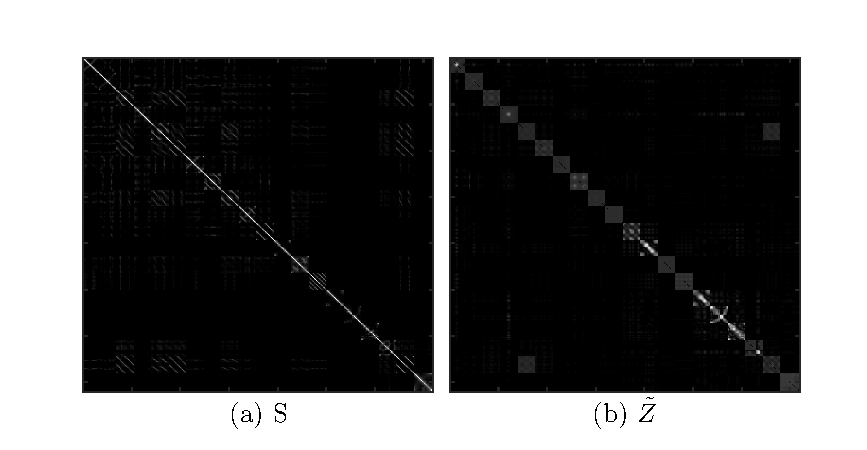
\includegraphics[width = 0.8\linewidth]{figure/COIL20_block.eps}
        \caption{A visual comparison of $S$ and $\tilde{Z}$ for \coil}
        \label{figure:COIL20_block}
        \vspace{-5mm}
\end{figure}

\comment{
\subsection{Parameter study}
Finally, we study the parameter sensitivity.
There exist three parameters in our method: $\lambda_1$, $\lambda_2$ and $K$.
$\lambda_1$ and 
$\lambda_2$ control the strength of Frobenius norm and the TKNN graph respectively.
$K$ is the number of nearest neighbors used to construct the TKNN graph.
We study these parameters by varying one and fixing others.
%We vary $\lambda_1$ in $[0.01,0.1,0.5,0.8,1,2,5,10]$ and 
%$\lambda_2$ in $[0, 0.001,0.005,0.008,0.01,0.05,0.1,1,10]$ respectively.
Experimental results are shown in Fig.~\ref{figure:para_study}.

\textbf{[Analysis on $\lambda_1$]} 
All the datasets exhibit similar results on $\lambda_1$, 
so we only show one case in Fig.~\ref{figure:para_study}(a).
With varying $\lambda_1$,
all the three lines rise first, keep stable and drop then.
When $\lambda_1$ is too small, some entries may be dominant in the rectified matrix, leading to poor performance. 
When $\lambda_1$ is too large, all the entries in the rectified matrix will be of similar values,
so clustering results will be unfavorable.

\textbf{[Analysis on $\lambda_2$]} 
Experimental results on $\lambda_2$ can be divided into three cases,
indicating different importance of the TKNN graph.
Three datasets \emph{glass}, \emph{seg\_7\textsc{class}} and \emph{COIL20} are given as examples
and their results are respectively shown in Fig.~\ref{figure:para_study}(b) - (d).
%In particular, we explore one more case $\lambda_1 = 100$ on \emph{glass} to show the overall trend.
%From these figures, we observe that 

\noindent{\small$\bullet$}
Fig.~\ref{figure:para_study}(b) shows the case that the TKNN graph will be of little use.
It occurs when the TKNN graph conveys redundant cluster-separation information contained in the raw similarity matrix.
Although ineffective similarities cannot be rectified,
ROSC can still reserve the effectiveness of effective similarities,
which ensures its robustness. 

\noindent{\small$\bullet$}
Fig.~\ref{figure:para_study}(c) describes the second case that 
the cluster-separation information
contained in the TKNN graph and in the raw similarity matrix complements each other.
As $\lambda_2$ increases,
the three lines first rise and then drop,
which demonstrates the importance of both the raw similarity matrix and the TKNN graph.

\noindent{\small$\bullet$}
The third case is depicted in Fig.~\ref{figure:para_study}(d) that
the TKNN graph contains sufficient cluster-separation information which covers that contained in the raw similarity matrix.
It is observed that 
the clustering results are gradually improved with the increase of $\lambda_2$ and finally keep stable.
%When $\lambda_2$ is large, the TkNN graph will dominate the results.
%In this case, the TKNN graph is so competitive that it covers the useful cluster-separation information 
%contained in the original similarity matrix.
In this case,
using only the TKNN graph can also perform well.

\textbf{[Analysis on $K$]}
We vary $K$ on datasets with useful TKNN graph
and get similar results as shown in Fig.~\ref{figure:para_study}(e),
where all the three lines rise first and drop then.
When $K$ is small,
objects in the same cluster but far away from each other will still be disconnected in the TKNN graph.
When $K$ is large,
it is more likely that objects in different clusters will be connected,
which ends up leading to disaster for clustering.

Although the TKNN graph may be of different importance on different datasets,
%there exists a certain range on both $\lambda_1$ and $\lambda_2$ where ROSC can achieve favorable clustering results in all cases,
%which proves the robustness of ROSC. 
setting $\lambda_1 = 1$, $\lambda_2 = 0.01$ and $K = 4$ works for most datasets used in our experiments.
}
\comment{
\begin{figure*}[!htbp]
    \subfloat[glass\label{figure:para_glass_l1}]{%
       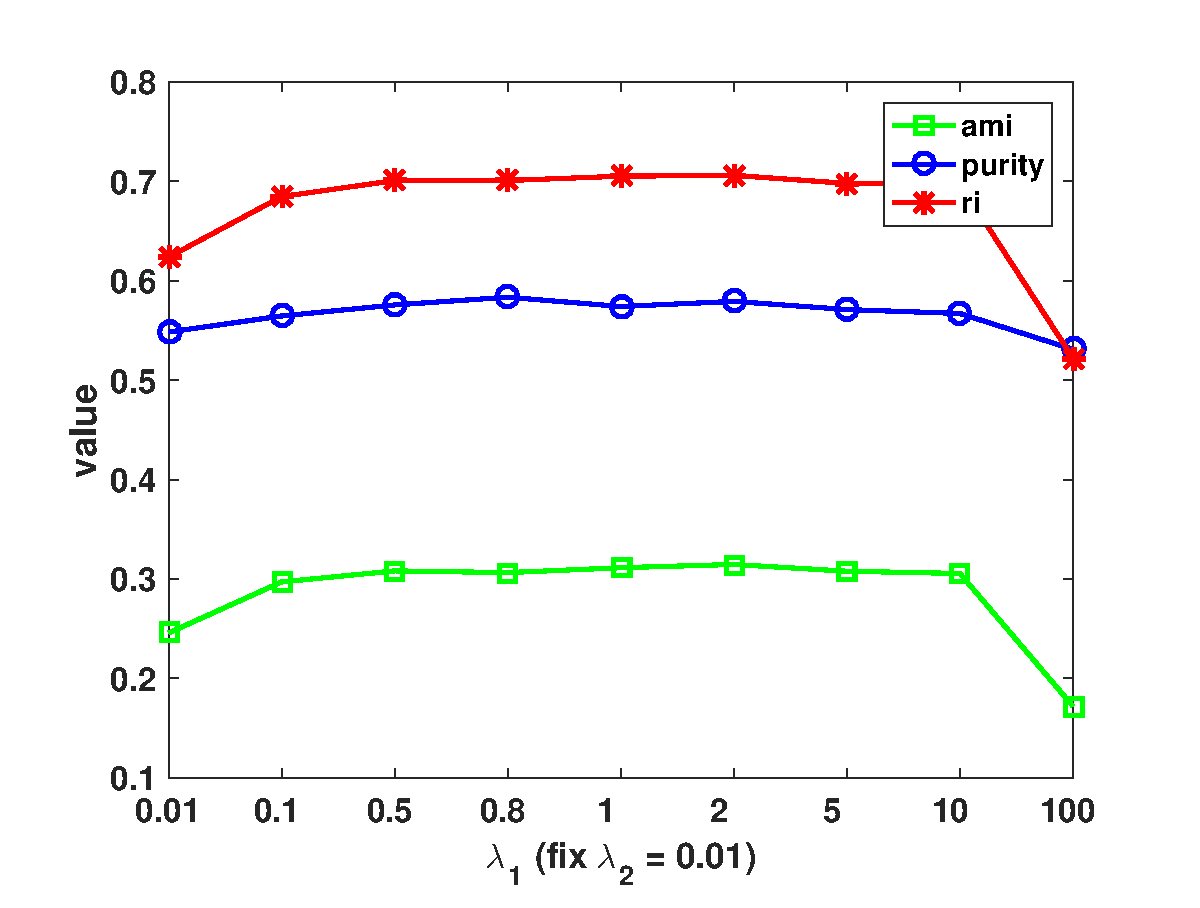
\includegraphics[width=0.33\textwidth]{figure/para_glass_l1.eps}
     }
    % \hfill
     \subfloat[isolet\label{figure:para_isolet_l1}]{%
       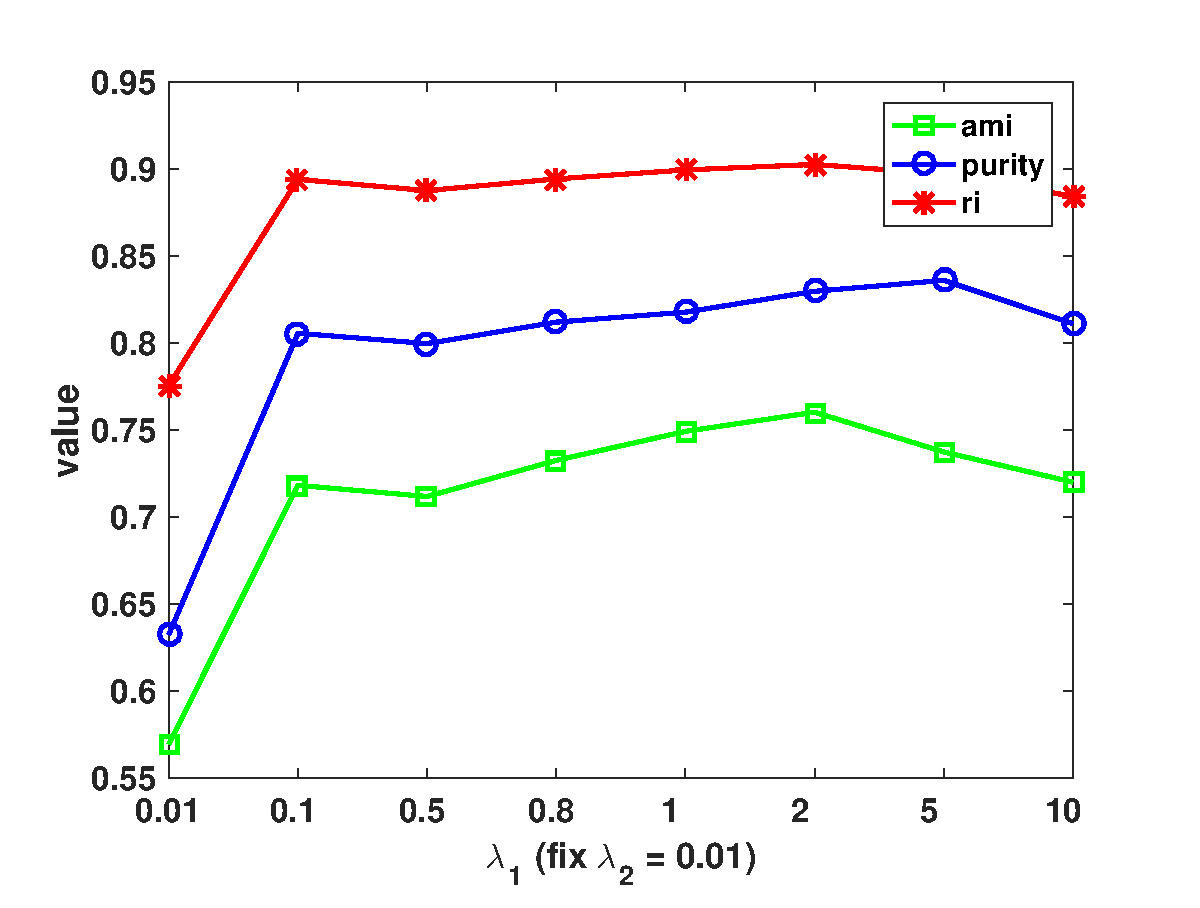
\includegraphics[width=0.33\textwidth]{figure/para_isolet_l1.eps}
     }
   %  \hfill
     \subfloat[COIL20\label{figure:para_COIL20_l1}]{%
       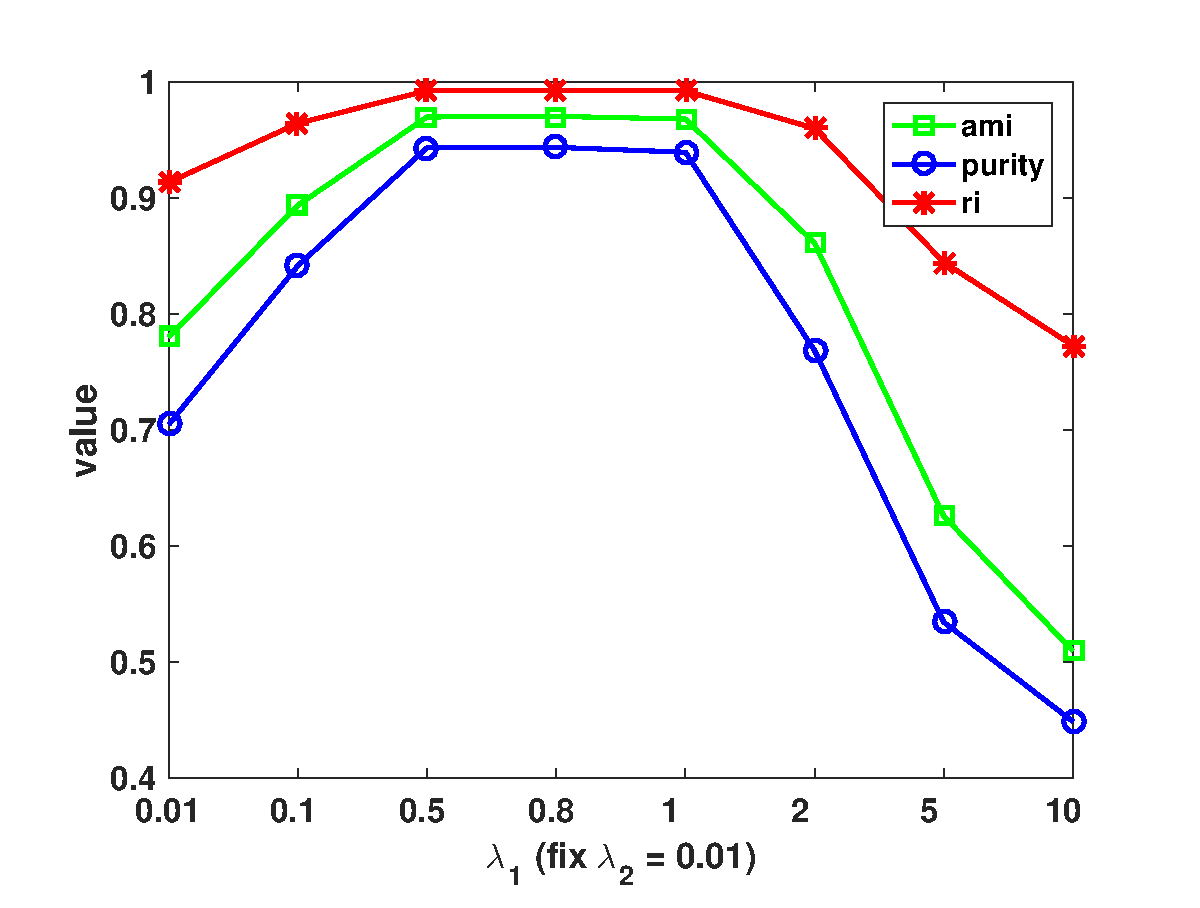
\includegraphics[width=0.33\textwidth]{figure/para_COIL20_l1.eps}
     }
     \caption{Study on parameter $\lambda_1$}
     \label{figure:paral1}
\end{figure*}

\begin{figure*}[!htbp]
    \subfloat[glass\label{figure:para_glass_l2}]{%
       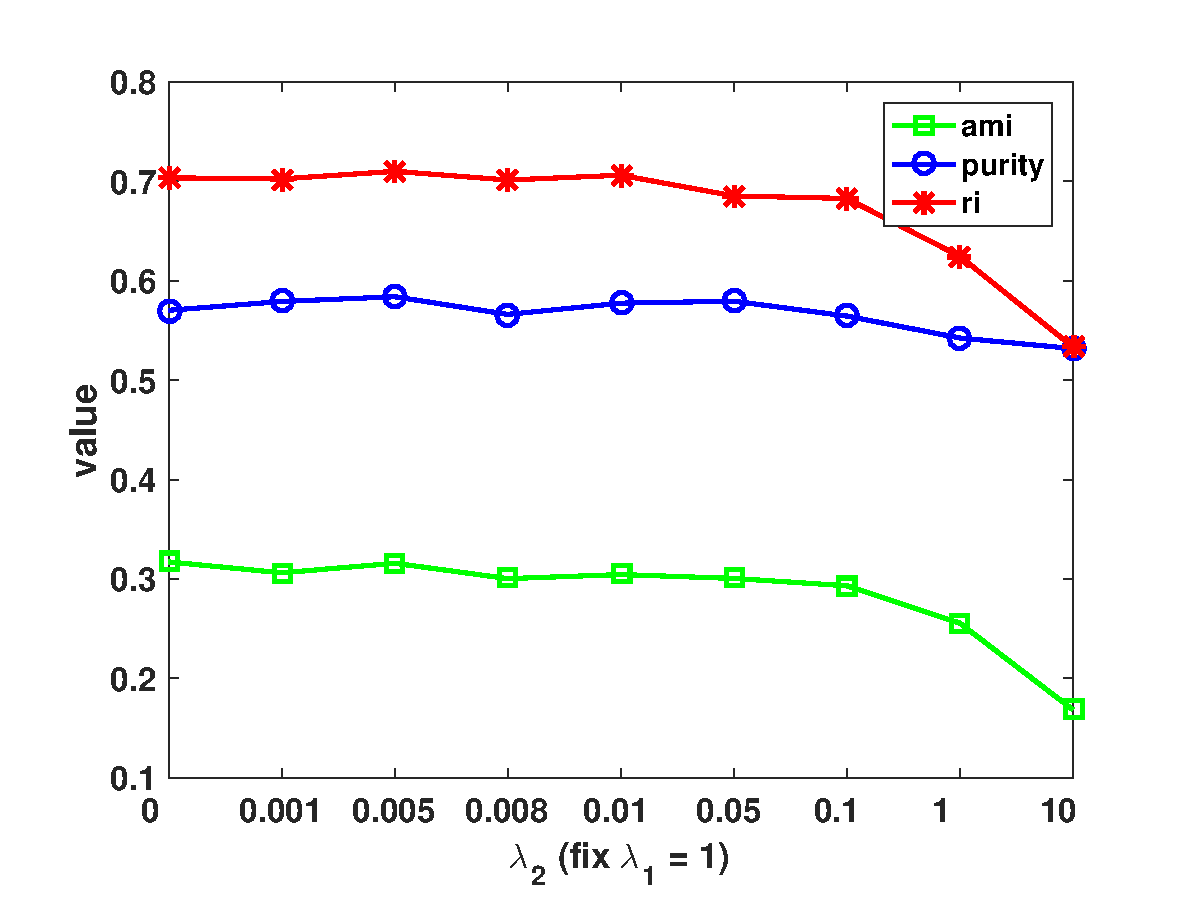
\includegraphics[width=0.33\textwidth]{figure/para_glass_l2.eps}
     }
  %   \hfill
     \subfloat[isolet\label{figure:para_isolet_l2}]{%
       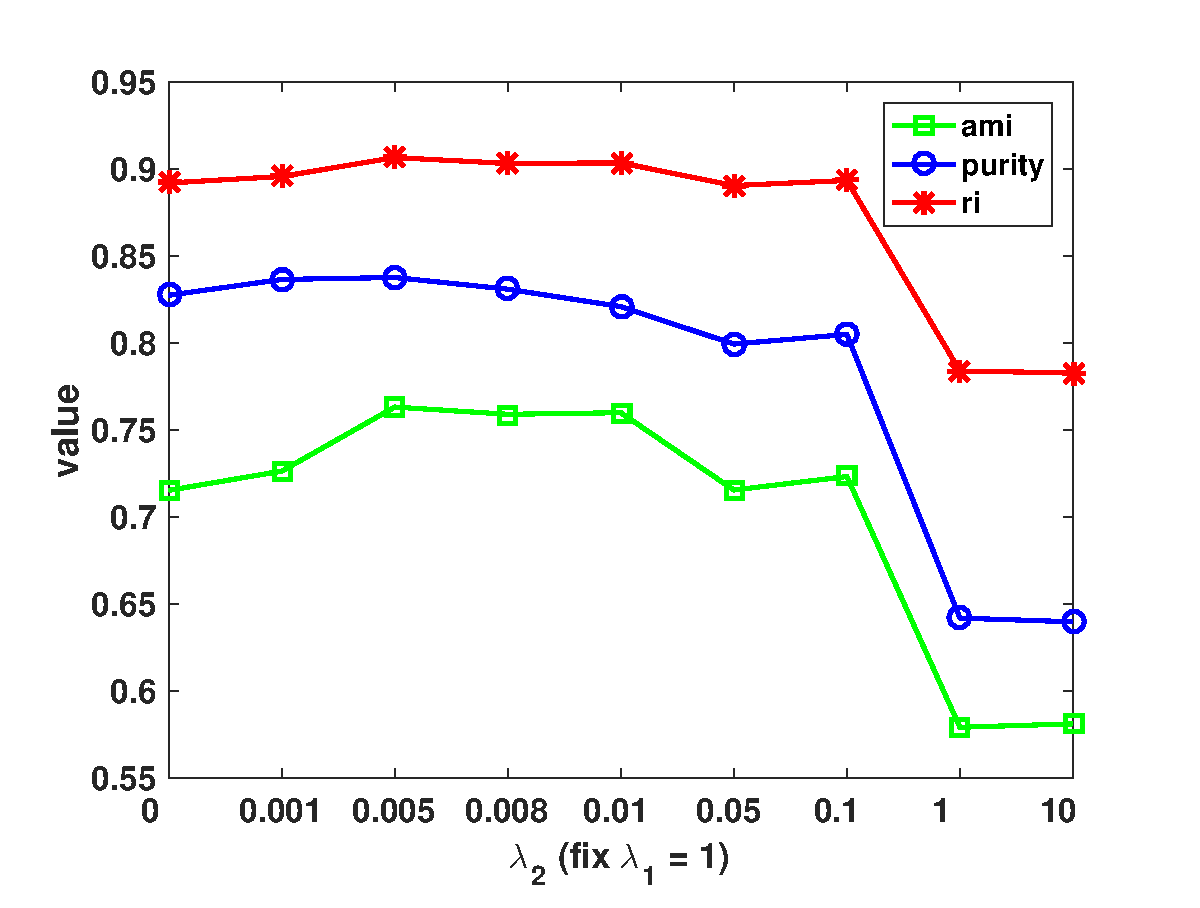
\includegraphics[width=0.33\textwidth]{figure/para_isolet_l2.eps}
     }
%     \hfill
     \subfloat[COIL20\label{figure:para_COIL20_l2}]{%
       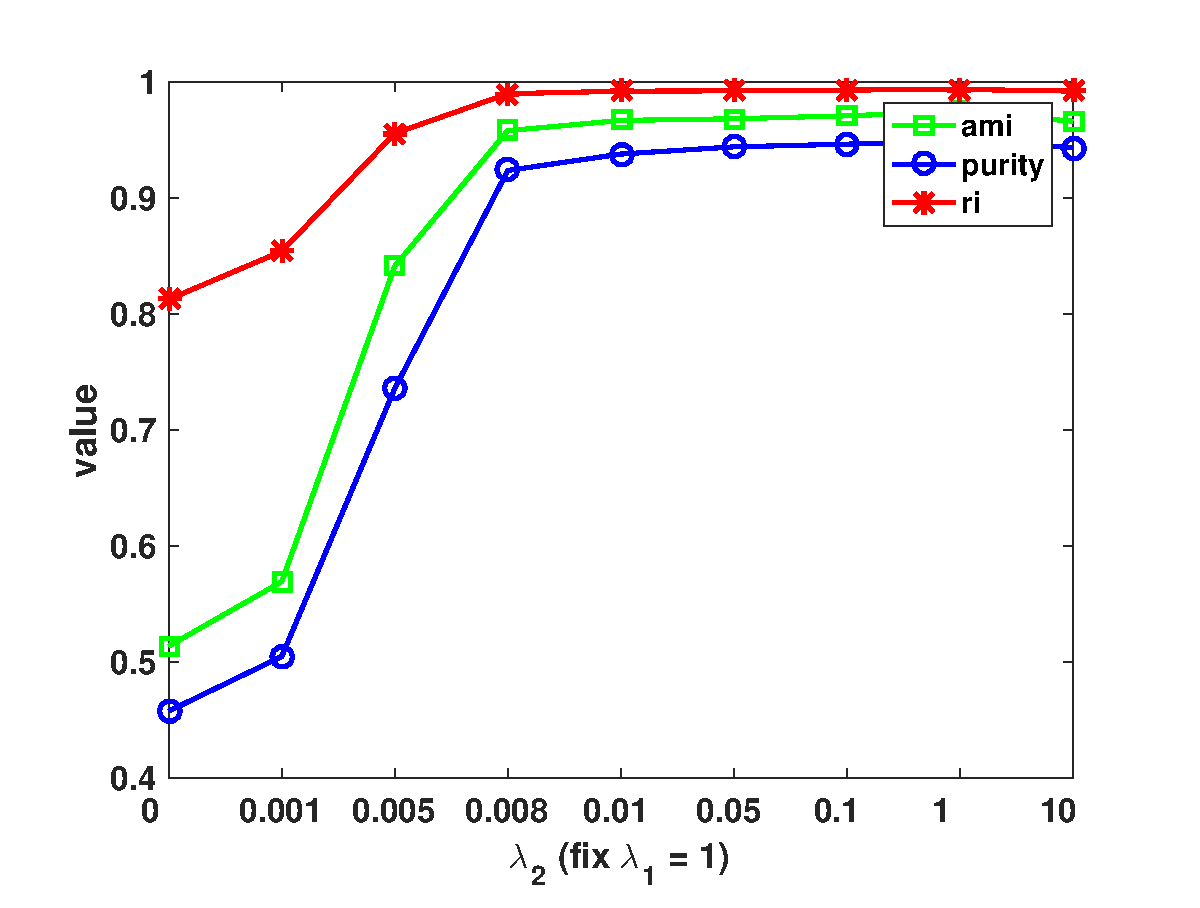
\includegraphics[width=0.33\textwidth]{figure/para_COIL20_l2.eps}
     }
     \caption{Study on parameter $\lambda_2$}
     \label{figure:paral2}
\end{figure*}
}

\comment{
\begin{figure*}[!htbp]
    \subfloat[$\lambda_1$(isolet)\label{figure:para_isolet_l1_new}]{%
       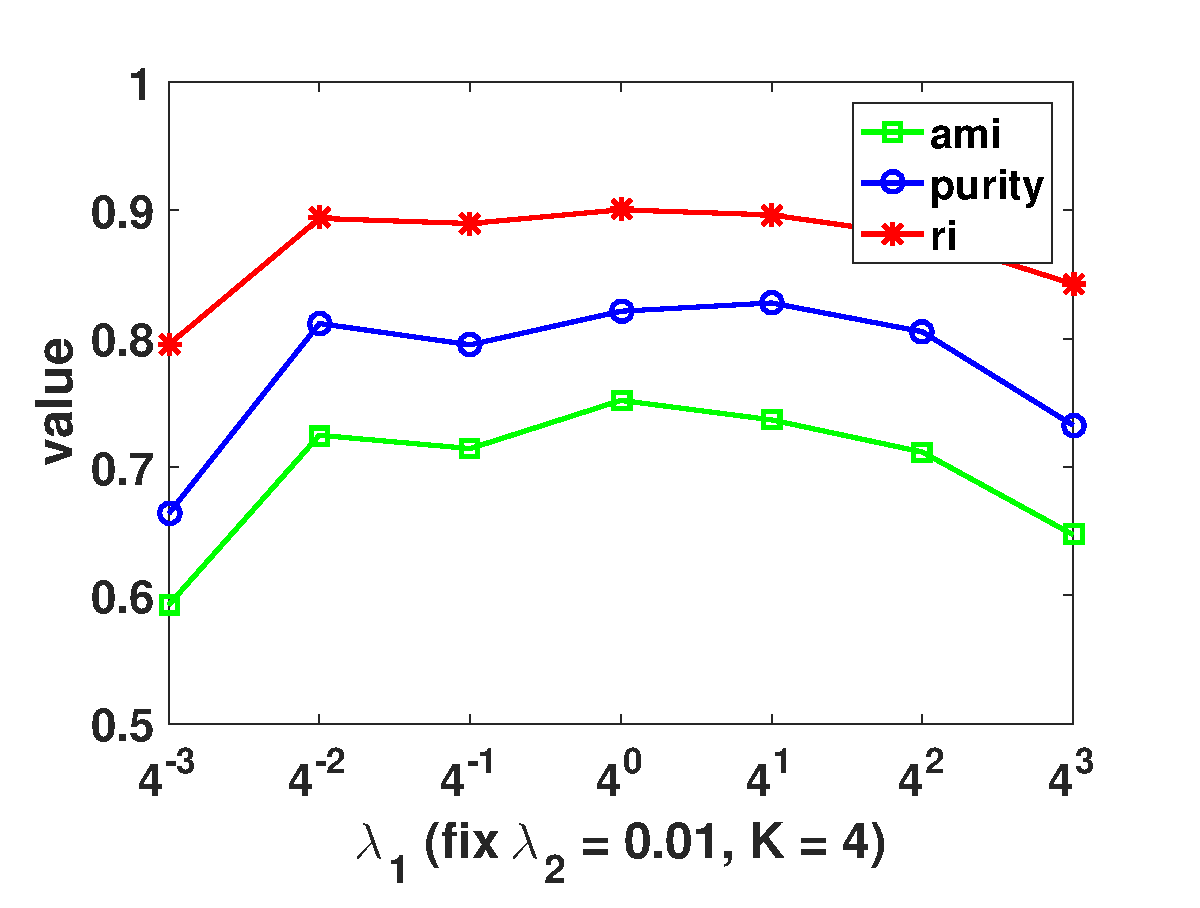
\includegraphics[width=0.2\textwidth]{figure/para_isolet_l1_new.eps}
     }
    \subfloat[$\lambda_2$(glass)\label{figure:para_glass_l2_new}]{%
       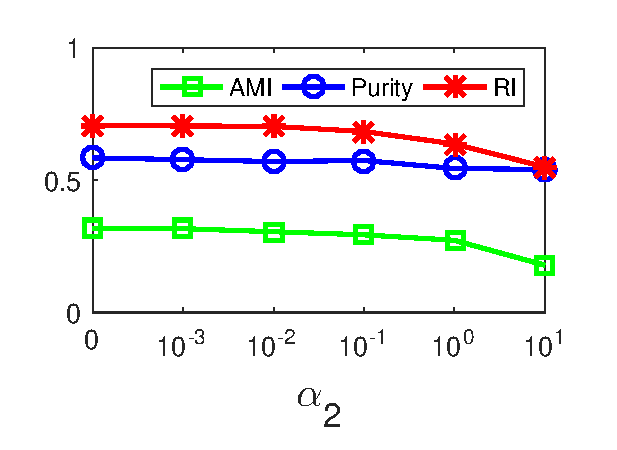
\includegraphics[width=0.2\textwidth]{figure/para_glass_l2_new.eps}
     }
     \subfloat[$\lambda_2$(seg\_\textsc{7class})\label{figure:para_seg_l2_new}]{%
       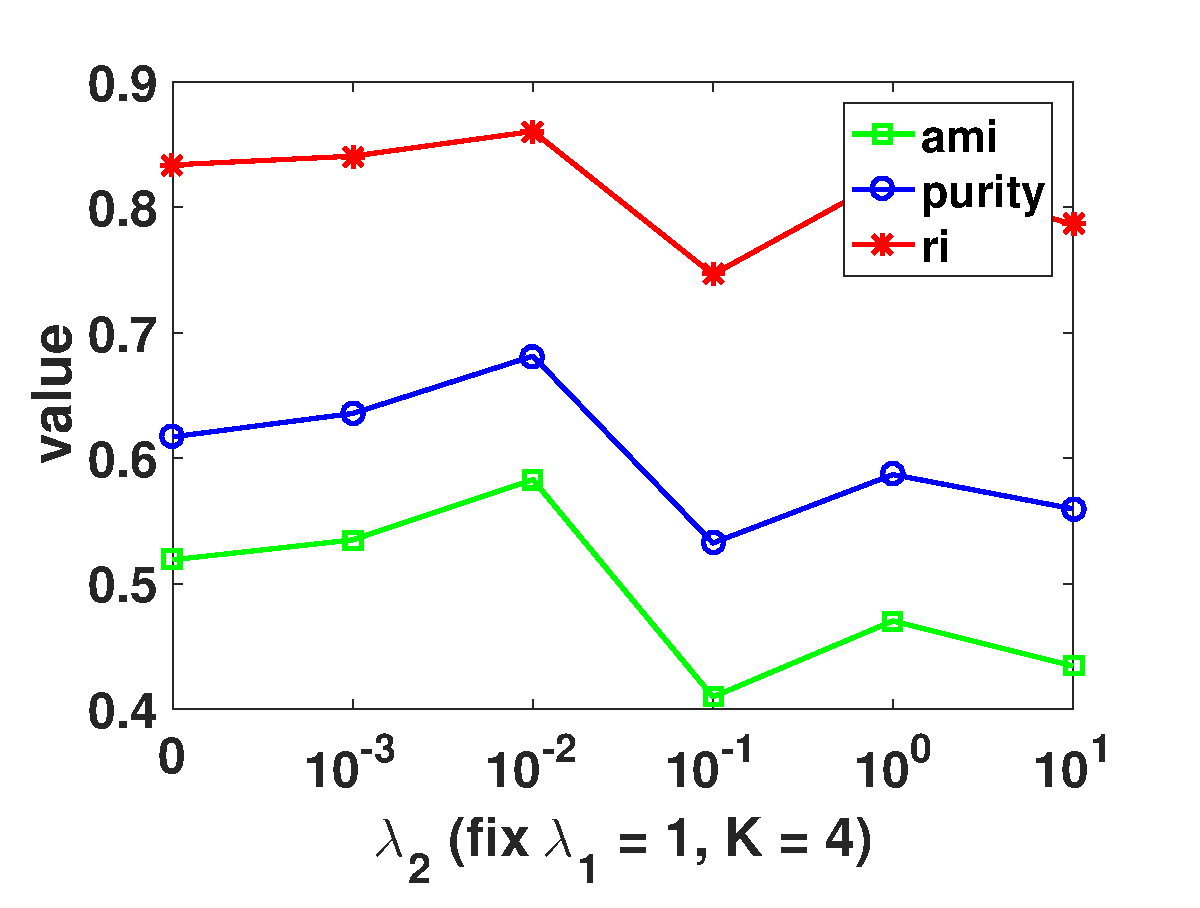
\includegraphics[width=0.2\textwidth]{figure/para_seg_l2_new.eps}
     }
   \subfloat[$\lambda_2$(COIL20)\label{figure:para_COIL20_l2_new}]{%
       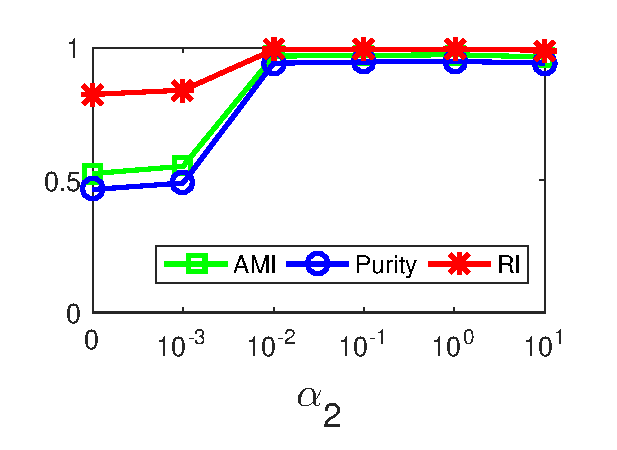
\includegraphics[width=0.2\textwidth]{figure/para_COIL20_l2_new.eps}
     }
     \subfloat[$K$(COIL20)\label{figure:para_K}]{%
       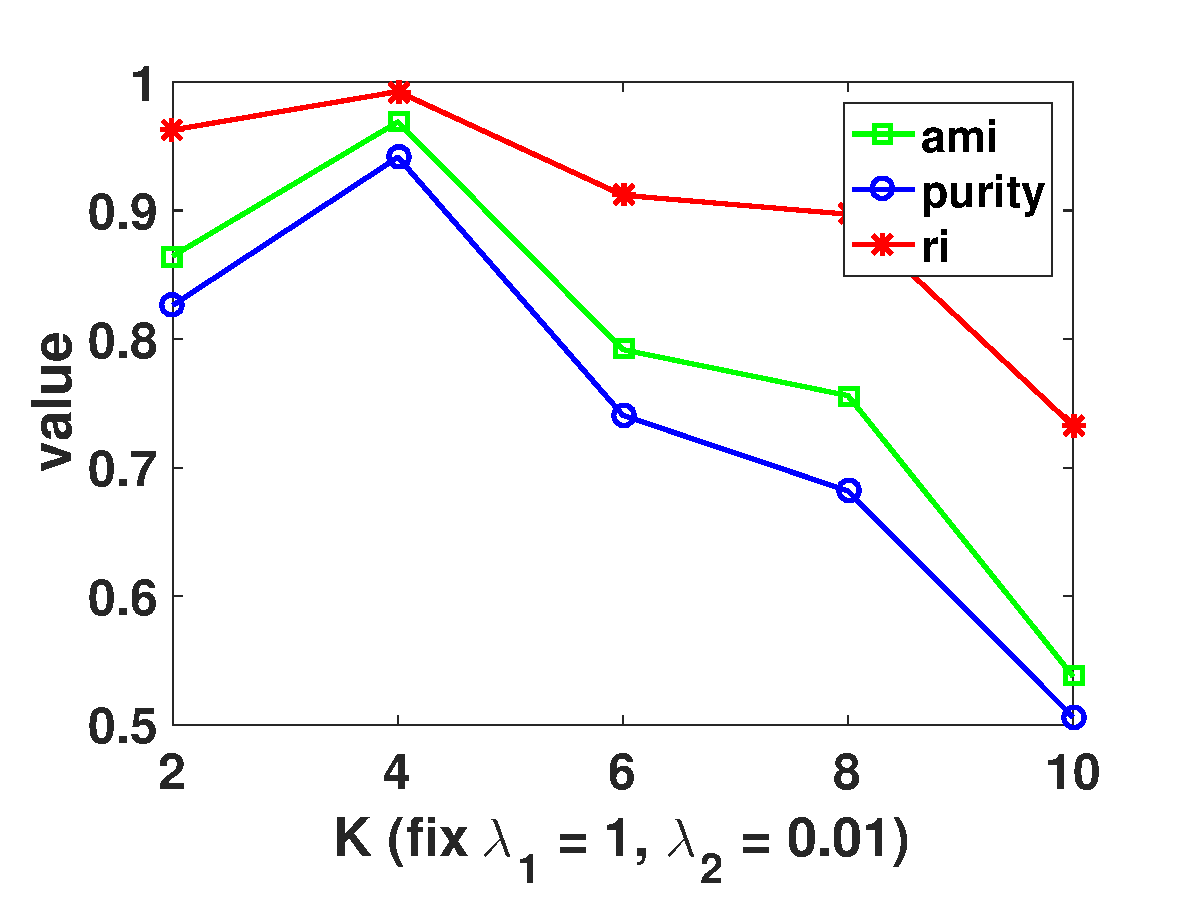
\includegraphics[width=0.2\textwidth]{figure/para_K.eps}
     }
     \caption{Parameter study on $\lambda_1$, $\lambda_2$ and $K$}
     \label{figure:para_study}
\end{figure*}
}

\begin{figure}[!htbp]
     \subfloat[COIL20 \label{figure:para_COIL20_l2_new}]{%
       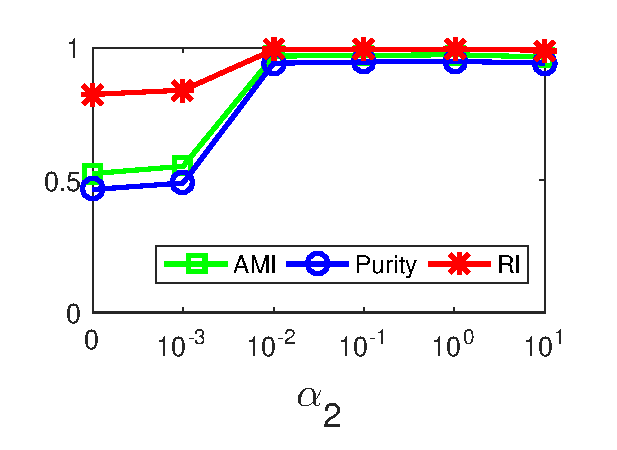
\includegraphics[width=0.22\textwidth]{figure/para_COIL20_l2_new.eps}
     }
     \subfloat[glass \label{figure:para_glass_l2_new}]{%
       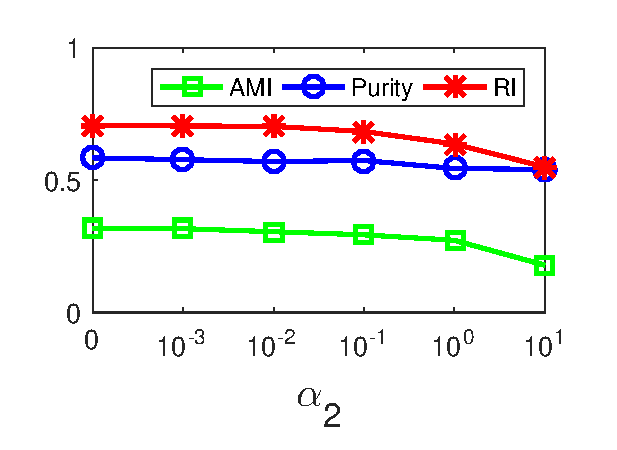
\includegraphics[width=0.22\textwidth]{figure/para_glass_l2_new.eps}
     }
     \vspace{-2mm}
    \caption{ROSC's performance scores vs. $\alpha_2$}
        \label{figure:lambda2}
        \vspace{-3mm}
\end{figure}


\noindent{\bf[TKNN graph]}
We end this section with a further discussion on the TKNN graph regularizing 
matrix $Z$ (via the reachability matrix $\mathcal{W}$).
From Equation~\ref{eq:obj_constraint}, we see that the degree of such regularization is 
controlled by the parameter $\alpha_2$. 
The larger $\alpha_2$ is, the more dominant is the TKNN graph regularization in
the objective function. 
Figures~\ref{figure:lambda2}(a) and (b) show the performance scores of ROSC 
as $\alpha_2$ varies for the dataset \coil\ and \glass, respectively. 
Note that the x-axes are shown in log scale. 
We note that trends of the curves in the two figures are quite different:
For \coil, the performance drops when $\alpha_2$ is very small, while for \glass, it is the other way
round.
The reason is that \coil\ is highly multi-scale (see Table~\ref{table:des_real}).
In particular, there are very big clusters whose objects could be at large distances from each other.
The TKNN graph has the effect of capturing the reachability similarities of these objects despite
their weak feature similarities, and hence maintain their strong correlations. 
At very small $\alpha_2$, the regularization effect is given too small a weight for it to
be effective, leading to smaller performance scores. 
For \glass, the dataset is much less multi-scale. 
The performance of ROSC stays very stable over a range of $\alpha_2$ values
until $\alpha_2$ becomes very large, in which case, reachability similarity
over-dominates  feature similarity, resulting in a mild dip in performance.

\comment{
\begin{figure}
    \centering
        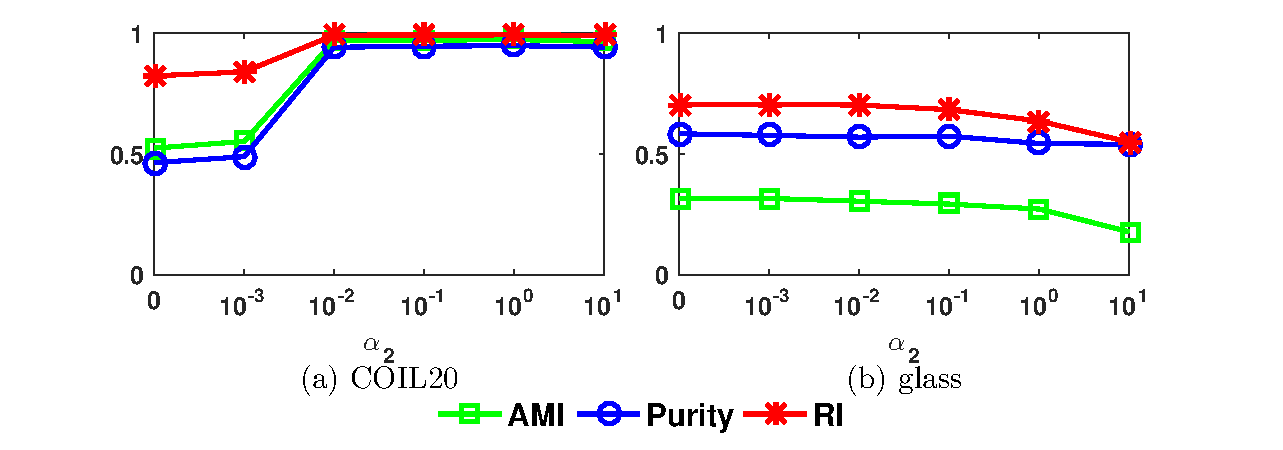
\includegraphics[width = \linewidth]{figure/para_analysis.eps}
        \caption{ROSC's performance scores vs. $\alpha_2$}
        \label{figure:lambda2}
\end{figure}}

\comment{
\subsection{Case study}
Finally, we conduct two case studies which apply ROSC to identify objects in images.
%especially in the case of multiple moving objects in video sequences.
%This is known as the motion segmentation problem.
%Motion segmentation is an important pre-processing step for several applications in computer vision, 
%such as tracking, action recognition, etc.
%It aims to segment multiple moving objects in a scene.
Fig.~\ref{fig:motion} shows two sample images from video sequences 
extracted from the well known Hopkins155 dataset~\cite{tron2007benchmark} for motion segmentation,
%which contains 155 video sequences along with the object features extracted and tracked in all the frames.
where tracked points in different motions are marked by different colors.
Taking motions as the ground truth, we cluster the tracked points and 
experimental results on the two images are respectively shown in Table~\ref{table:motion1} and~\ref{table:motion2}.
We observe that ROSC greatly outperforms other baseline methods with regard to all the three measures,
which proves its ability in object identification and sheds some light on its applicability in improving motion segmentation.

\begin{figure}[!htbp]
    \subfloat[\label{fig:motion1}]{%
       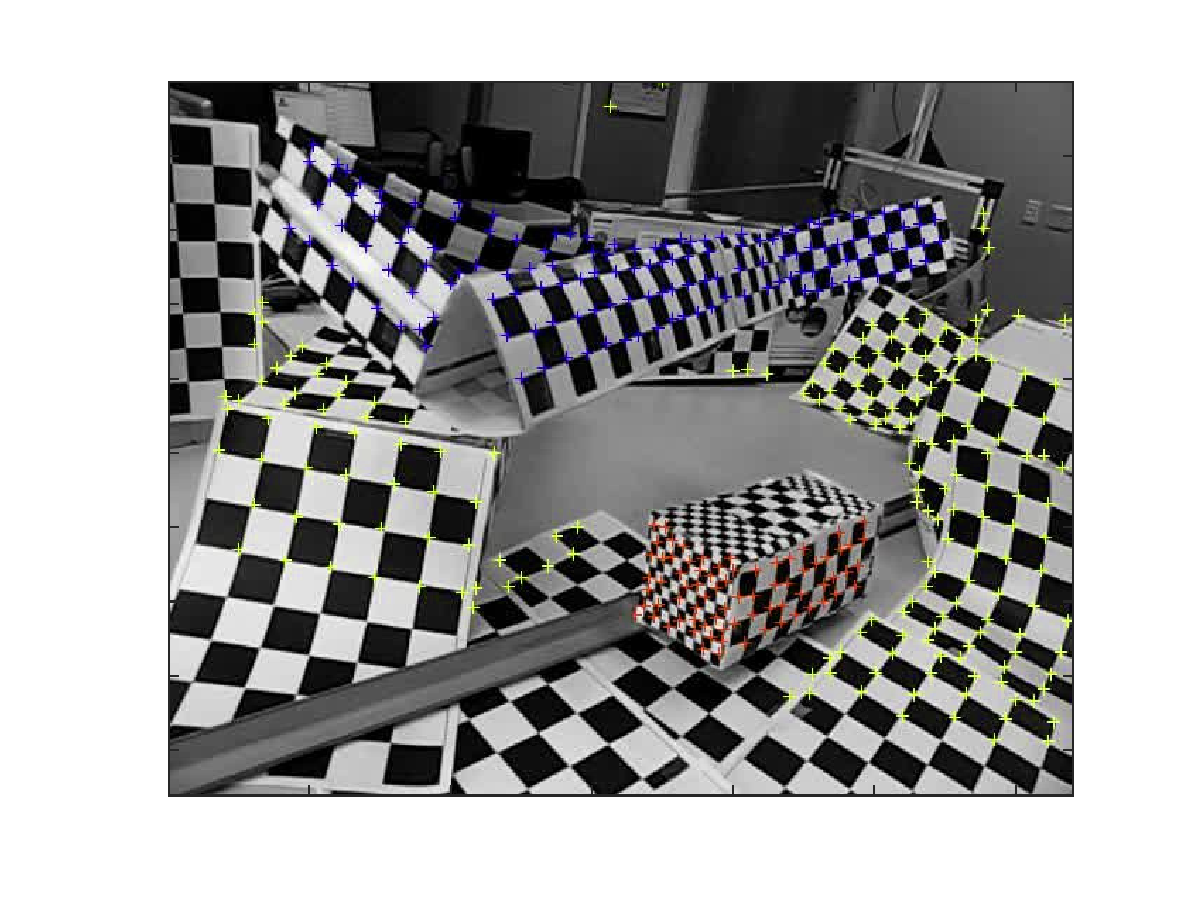
\includegraphics[width=0.25\textwidth]{figure/motion1.eps}
     }
  %   \hfill
     \subfloat[\label{fig:motion2}]{%
       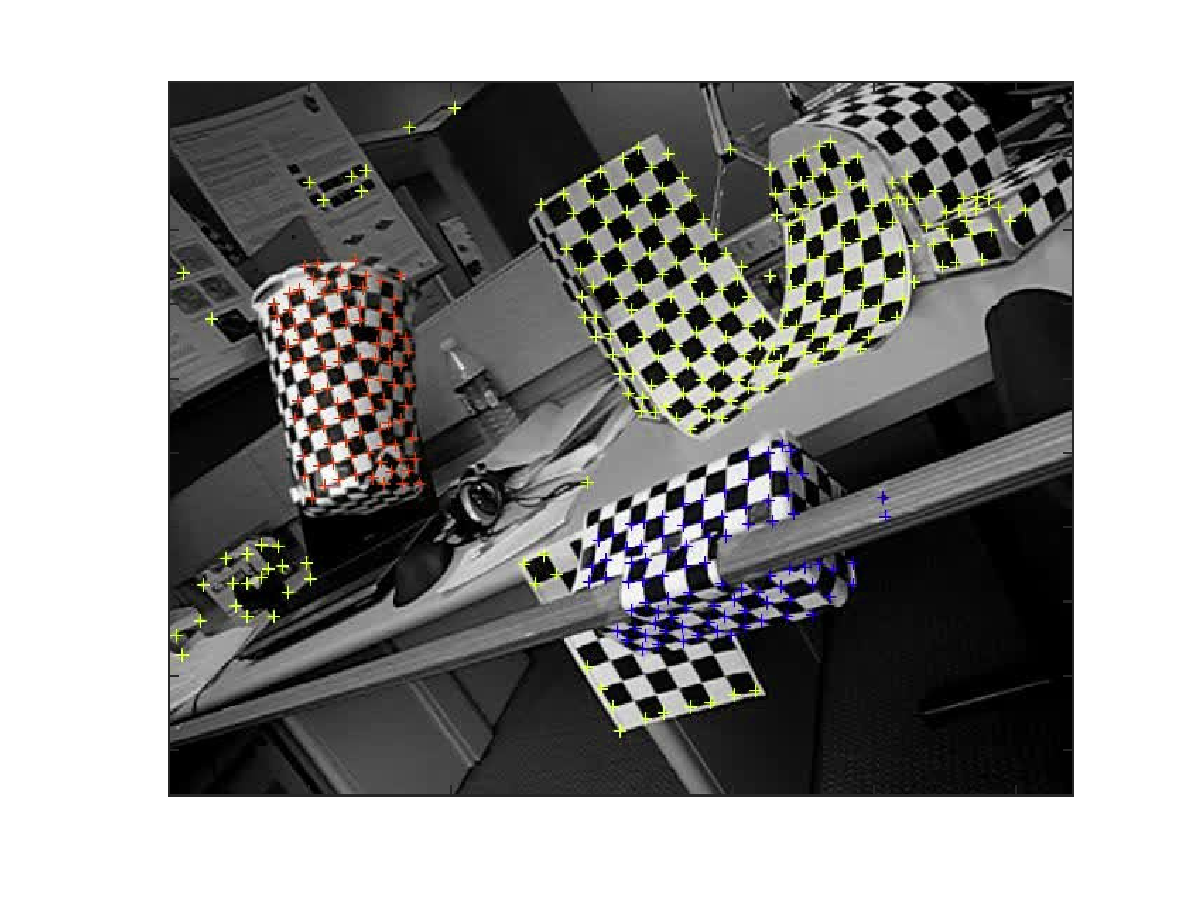
\includegraphics[width=0.25\textwidth]{figure/motion2.eps}
     }
     \caption{Toy image examples}
     \label{fig:motion}
\end{figure}

\comment{
\begin{figure}[!htbp]
    \centering
    \begin{minipage}{0.25\textwidth}
        \centering
        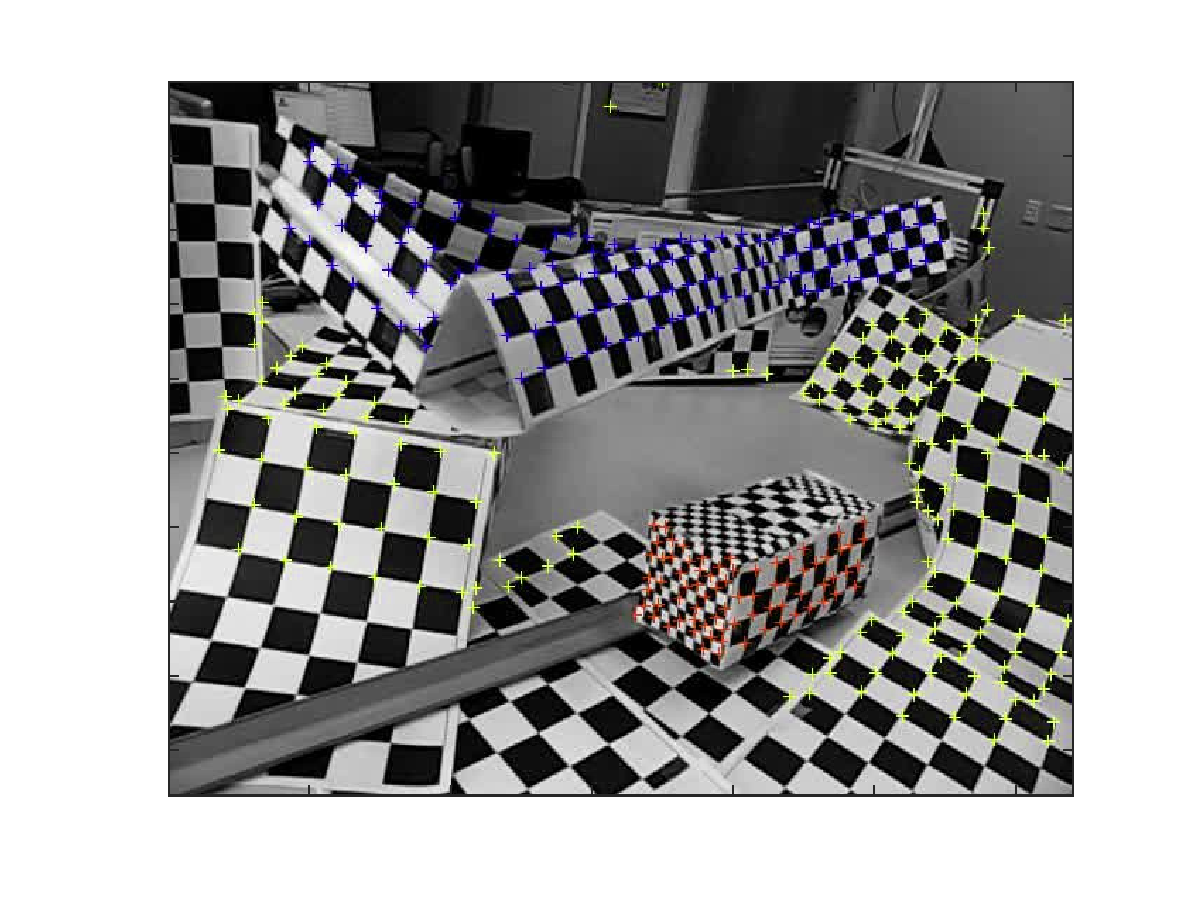
\includegraphics[width=1.1\textwidth]{figure/motion1.eps}
        %\caption{$dt=0.1$}
        \label{fig:motion1}
    \end{minipage}%
    \begin{minipage}{0.25\textwidth}
        \centering
        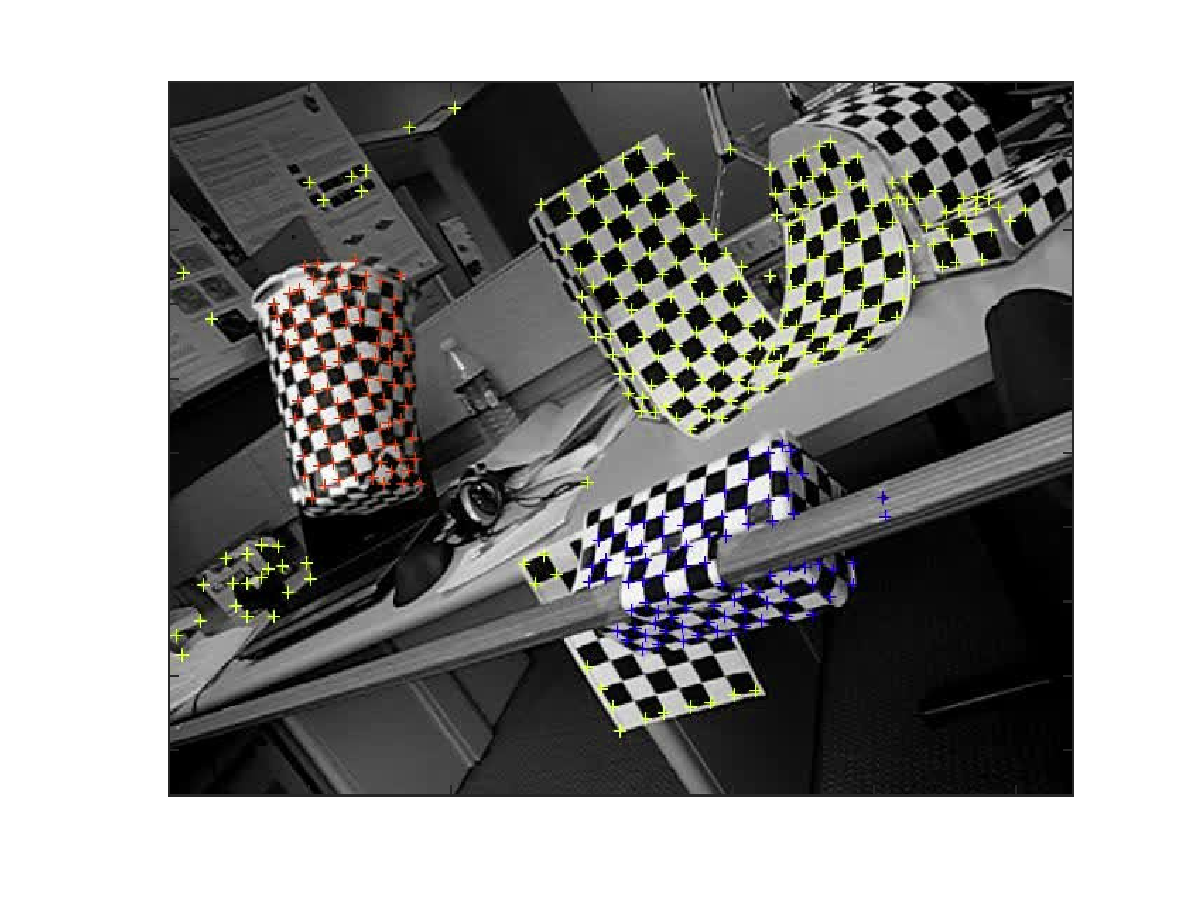
\includegraphics[width=1.1\textwidth]{figure/motion2.eps}
        %\caption{$dt =$}
        \label{fig:motion2}
    \end{minipage}
    \caption{Toy image examples}
     \label{fig:motion}
\end{figure}
}

\begin{table*}[!htbp]
\centering
\caption{Clustering results on Fig.~\ref{fig:motion}(a)}
\label{table:motion1}
\resizebox{0.8\linewidth}{!}
{
\begin{tabular}{|c|c|c|c|c|c|c|c|c|c|c|} \hline
Measure &NJW & NCuts & ZP & PIC & PIC-$k$ & DPIC & DPIE & FUSE & ROSC \\ \hline 
AMI    & $0.3156$ & $0.3146$ & $0.3141$ & $0.3356$ & $0.3770$ & $0.1563$ & $0.1664$ & $0.4573$ & $\bm{0.7265}$ \\ \hline
Purity & $0.5694$ & $0.5651$ & $0.5645$ & $0.6337$ & $0.6444$ & $0.5121$ & $0.5663$ & $0.7100$ & $\bm{0.8613}$ \\ \hline
RI       & $0.6316$ & $0.6309$ & $0.6310$ & $0.6488$ & $0.6682$ & $0.5874$ & $0.4956$ & $0.6947$ & $\bm{0.8287}$ \\ \hline
\end{tabular}
}
\caption{Clustering results on Fig.~\ref{fig:motion}(b)}
\label{table:motion2}
\resizebox{0.8\linewidth}{!}
{
\begin{tabular}{|c|c|c|c|c|c|c|c|c|c|c|} \hline
Measure &NJW & NCuts & ZP & PIC & PIC-$k$ & DPIC & DPIE & FUSE & ROSC \\ \hline 
AMI    & $0.6900$ & $0.6900$ & $0.6900$ & $0.5157$ & $0.6082$ & $0.5983$ & $0.0679$ & $0.6352$ & $\bm{0.8131}$ \\ \hline
Purity & $0.9000$ & $0.9000$ & $0.9000$ & $0.7736$ & $0.8334$ & $0.8402$ & $0.5757$ & $0.8467$ & $\bm{0.9464}$ \\ \hline
RI       & $0.8586$ & $0.8586$ & $0.8586$ & $0.7364$ & $0.7958$ & $0.7978$ & $0.4245$ & $0.8027$ & $\bm{0.9227}$ \\ \hline
\end{tabular}
}
\end{table*}
}

\section{Conclusions}
In this paper we studied the effectiveness of semi-supervised classification methods in handling heterogeneous information network data.
\label{sec:conclusion}




%\end{document}  % This is where a 'short' article might terminate

% ensure same length columns on last page (might need two sub-sequent latex runs)

%ACKNOWLEDGMENTS are optional

\section{Acknowledgments}
This research is supported by Hong Kong Research Grants Council GRF HKU 17254016.

\newpage

% The following two commands are all you need in the
% initial runs of your .tex file to
% produce the bibliography for the citations in your paper.
\bibliographystyle{ACM-Reference-Format}

%\bibliographystyle{abbrv}
\balance

\bibliography{hingcn}  % vldb_sample.bib is the name of the Bibliography in this case
% You must have a proper ".bib" file
%  and remember to run:
% latex bibtex latex latex
% to resolve all references

%APPENDIX is optional.
% ****************** APPENDIX **************************************
% Example of an appendix; typically would start on a new page
%pagebreak


\end{document}
